% shtthesis, an unofficial LaTeX thesis template for ShanghaiTech University.
% Copyright (C) 2022 Li Rundong <rundong.001@gmail.com>
%
% This program is free software: you can redistribute it and/or modify
% it under the terms of the GNU General Public License as published by
% the Free Software Foundation, either version 3 of the License, or
% (at your option) any later version.
%
% This program is distributed in the hope that it will be useful,
% but WITHOUT ANY WARRANTY; without even the implied warranty of
% MERCHANTABILITY or FITNESS FOR A PARTICULAR PURPOSE.  See the
% GNU General Public License for more details.
%
% You should have received a copy of the GNU General Public License
% along with this program.  If not, see <https://www.gnu.org/licenses/>

% graduate setup
% \documentclass[master,anonymous]{shtthesis}
\documentclass[master]{shtthesis}
\shtsetup{
  anonymous-str = XXX,
  degree-name = {工学硕士},
  degree-name* = {Master~of~Science~in~Engineering},
  secret-level = {},
  title = {面向计算机视觉算法部署的延迟观测},
  title* = {Latency Observation Towards Computer Vision Algorithm Deployment},
  keywords = {计算机视觉,算法部署,延迟观测,边缘计算,日志系统},
  keywords* = {Computer Vision, Algorithm Deployment,Latency Observation,Edge Computing,Log System},
  author = {方海舟},
  author* = {Fang~Haizhou},
  institution = {上海科技大学信息科学与技术学院},
  institution* = {School~of~Information~Science~and~Technology\\%
                  ShanghaiTech~University},
  supervisor = {范睿~副教授},
  supervisor* = {Professor~Fan~Rui},
  supervisor-institution = {上海科技大学信息科学与技术学院},
  discipline-level-1 = {计算机科学与技术},
  discipline-level-1* = {Computer~Science~and~Technology},
  bib-resource = {myref.bib},
}

\usepackage{listings}
\usepackage{bicaption}
\captionsetup[figure][bi-first]{name=图}
\captionsetup[figure][bi-second]{name=Figure}
\captionsetup{font={small,bf,stretch=1.5},justification=raggedright}
\captionsetup[table][bi-first]{name=表}
\captionsetup[table][bi-second]{name=Table}
\newcommand\prompt{\textup{\$}}
\lstdefinestyle{lstStyleBase}{%
  basicstyle=\small\ttfamily,
  aboveskip=\medskipamount,
  belowskip=\medskipamount,
  lineskip=0pt,
  boxpos=c,
  showlines=false,
  extendedchars=true,
  upquote=true,
  tabsize=2,
  showtabs=false,
  showspaces=false,
  showstringspaces=false,
  numbers=none,
  linewidth=\linewidth,
  xleftmargin=4pt,
  xrightmargin=0pt,
  resetmargins=false,
  breaklines=true,
  breakatwhitespace=false,
  breakindent=0pt,
  breakautoindent=true,
  columns=flexible,
  keepspaces=true,
  gobble=0,
  framesep=3pt,
  rulesep=1pt,
  framerule=1pt,
  frame=l,
  rulecolor=\color{ShtRed},
  backgroundcolor=\color{gray!5},
  stringstyle=\color{green!40!black!100},
  keywordstyle=\bfseries\color{blue!50!black},
  commentstyle=\slshape\color{black!60},
  escapeinside={`'},
}
\lstdefinestyle{lstStyleShell}{%
  style=lstStyleBase,
  language=bash}
\lstdefinestyle{lstStyleLaTeX}{%
  style=lstStyleBase,
  language=[LaTeX]TeX}
\lstnewenvironment{latex}{\lstset{style=lstStyleLaTeX}}{}
\lstnewenvironment{shell}{\lstset{style=lstStyleShell}}{}

\usepackage{hologo}
\usepackage{float}
\ifluahbtex
  \usepackage{emoji}
\else
  \providecommand{\emoji}[1]{ \fbox{\emph{#1}} }
\fi

\usepackage{subcaption}
\usepackage{ctable}
\usepackage[list=off]{bicaption}
\captionsetup[figure][bi-second]{name=Figure}
\captionsetup[table][bi-second]{name=Table}

\usepackage{listings}
\usepackage{xcolor}
\lstset{
	language = C++,
	backgroundcolor = \color{yellow!10},    % 背景色:淡黄
	basicstyle = \small\ttfamily,           % 基本样式 + 小号字体
	rulesepcolor= \color{gray},             % 代码块边框颜色
	breaklines = true,                  % 代码过长则换行
	numbers = left,                     % 行号在左侧显示
	numberstyle = \small,               % 行号字体
	keywordstyle = \color{blue},            % 关键字颜色
	commentstyle =\color{green!100},        % 注释颜色
	stringstyle = \color{red!100},          % 字符串颜色
	frame = shadowbox,                  % 用(带影子效果)方框框住代码块
	showspaces = false,                 % 不显示空格
	columns = fixed,                    % 字间距固定
	%escapeinside={<@}{@>}              % 特殊自定分隔符:<@可以自己加颜色@>
	morekeywords={cudaDeviceProp,cudaGetDeviceProperties,cudaDeviceGetUtilizationRates},                % 自加新的关键字(必须前后都是空格)
}


\makeatletter
  \def\ifundergraduate{\ifsht@undergraduate}
  \def\ifgraduate{\ifsht@graduate}
\makeatother
\begin{document}

\maketitle

\frontmatter
\begin{abstract}[flattitle]
近年来,受益于不断扩大的产业规模和持续增加的研究投入,计算机视觉算法在工业场景的应用取得了极大拓展,这对算法性能和可靠性提出了更高的需求。除去不断提升模型的推理准确性等指标以外,算法部署部分的优化也成为工程落地的重要环节。

为了满足工业应用场景低延迟,高可用的需求,以及提供故障后的追踪分析能力,提升算法的可靠性,作为一个重要的参考数据,计算机视觉算法在各个环节的运行延迟,通常需要被追踪和记录。但因为部署系统在硬件,软件方面的复杂性,以及安防、政府业务等隐私保护需求,实际工程项目中,传统运维观测方式有较大的局限性。

本文提出了一种面向计算机视觉算法部署阶段的延迟观测方案,其主要目的是解决传统日志观测方式在复杂部署条件下,观测维度和灵活度不足的问题。主要贡献为设计和实现了一种面向计算机视觉任务的延迟观测方案,其通过设计定制化的存储方式,并引入基于T-digest的分布估计算法实现过滤效果,节约了延迟观测结果的记录开销。同时,通过利用基于内核新特性的BPF技术,不仅实现了日志进程和程序主体的分离,还拓展了观测维度。

根据论文所述方案所开发的软件项目,被实践于具体的工程项目场景中,并在生产环境中取收益。在获得相关发明专利的同时,部分模块还迁移到内核IO观测场景,贡献于华为OpenEuler开源操作系统项目中。
\end{abstract}

\begin{abstract*}[flattitle]
In recent years, benefiting from the ever-expanding industrial scale and increasing research investment, the application of computer vision algorithms has been greatly expanded, which puts forward higher requirements for algorithm performance and reliability. In addition to continuously improving the  inference accuracy of the model and other indicators, the optimization of the algorithm deployment has also become an important part of the implementation.

In order to meet the low-latency and high-availability requirements of industrial applications, and to provide post-failure tracking and improve the reliability of algorithms as important reference data, the runtime latency of computer vision algorithms at each stage usually needs to be tracked and recorded. However, due to the complexity of its own system in terms of hardware and software, as well as the privacy requirements of security tasks and government business, in actual engineering projects, the traditional operation and maintenance monitoring method has great limitations.

This paper proposes a latency observation scheme for the deployment of computer vision algorithms, aims to solve the problem of insufficient observation dimensions and flexibility in traditional log observation methods under complex software/hardware conditions. The main contribution is a design and implementation of a lightweight latency observation tools for computer vision algorithms deployment, which reducing the observation results storage overhead through customized format and a distribution estimation algorithm (T-digest) based filter. At the same time, by using the BPF technology of the new kernel feature, not only the separation of the log process and the program is achieved, but also the observation dimension is expanded.

The software projects developed according to the scheme described in the paper are practiced in specific engineering project scenarios and gain benefits in the production environment. While obtaining related invention patents, some modules have also been migrated to the kernel IO observation scene and contributed to the Huawei OpenEuler open source operating system project.

\end{abstract*}

\makeindices

\ifgraduate
\begin{nomenclatures}[缩写]
  \header{缩写}{全称}
  \item{ASIC}{Application Specific Integrated Circuit}
  \item{FPGA}{Field Programmable Gate Arrays}
  \item{NMS}{Non-maximum Suppression}
  \item{AVX}{Advanced Vector Extensions}
  \item{CUDA}{Compute Unified Device Architecture}
  \item{SIMD}{Single Instruction Multiple Data}
  \item{FMA}{Fused Multiply Add}
  \item{RPC}{Remote Procedure Call}
  \item{RGB}{Red Green Blue}
  \item{HSV}{Hue Saturation Value}
  \item{QOS}{Quality of Service}
  \item{CPU}{Central Processing Unit}
  \item{GPU}{Graphics Processing Unit}
  \item{CUPTI}{CUDA Profiling Tools Interface}
  \item{GUI}{Graphical User Interface}
  \item{NPU}{Neural Network Processing Unit}
  \item{SDK}{Software Development Kit}
  \item{I/O}{Input/Output}
  \item{BPF}{Berkeley Packet Filter}
  \item{DAG}{Directed Acyclic Graph}
  \item{USDT}{User Statically-Defined Tracing}
  \item{OCR}{Optical Character Recognition}
\end{nomenclatures}

\fi

\mainmatter
\chapter{绪论}

\section{当代计算视觉算法的应用场景}\label{当代计算视觉算法的应用场景}

近年来,受益于深度学习\cite{lecun2015deep}的快速进步,当下计算机视觉算法已经超过了传统数字信号处理的应用范畴,除去在影像层面进行基础的滤波,去噪等\cite{dabov2007image},还拓展到了各种更有挑战性的场景,包括自动驾驶\cite{chen2015deepdriving},交通监控分析\cite{santos2020real},场地安防\cite{wang2019deep},医学影像处理\cite{litjens2017survey}等。以ImageNet\cite{deng2009imagenet}为起点,深度学习算法在众多场景下已经取得了显著的进展,成为了当代处理视觉任务的主流方法。目前的计算机服务器资源中,用于深度学习推理的部分也在迅速增加,从硬件设备侧看,近六年来累计出货AI服务器超过50万台,算力总规模达到202EFlops,全球占比33$\%$,其中智能算力增速超过85$\%$\cite{china2022}。在算力网络的层次中,基于云边协同的多设备协作体系正在不断扩大商用规模,边缘计算部署的比例不断提升,混合部署已然成为趋势。

\begin{figure}[htbp]
	\centering
	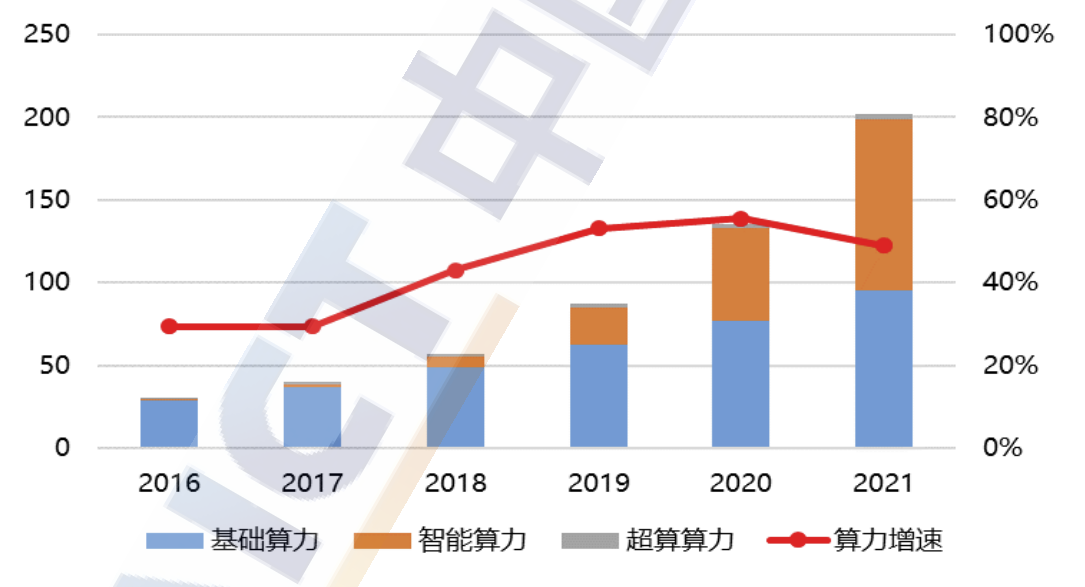
\includegraphics[width=8cm]{img/1.png}
	\bicaption{2022年中国算力发展状况\citep{china2022}}{China's computing power development status in 2022}
	\label{2022年中国算力发展状况}
\end{figure}

\section{计算机视觉算法工业化部署的特点与挑战}\label{计算机视觉算法工业化部署的特点与挑战}
\subsection{计算机视觉算法模型的生产过程}
当前主流的计算机视觉算法,大多是基于监督学习的深度神经网络模型。通常,会使用标注过的图像数据集来训练算法,使其能在特定的业务场景下,可以从输入数据中提取特征并做出正确的预测。具体的,一个基本的模型开发过程,通常会先构造一个带有标注的基础数据集,并将其分为用于训练和调整模型参数的训练集(Train Set),用来做模型选择的验证集(Validation Set),和最终评估模型的测试集(Test Set)。模型经过反复调整后,当算法工程师在测试集上取得理想的结果,则模型生产的部分就基本结束。

\begin{figure}[htbp]
	\centering
	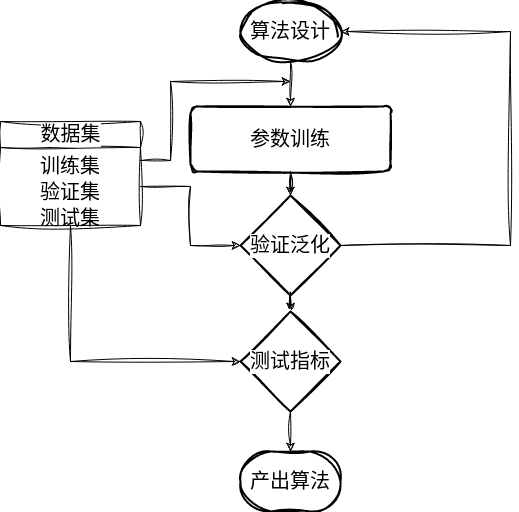
\includegraphics[width=8cm]{img/2.png}
	\bicaption{计算机视觉算法模型的生产过程}{The production process of computer vision algorithm model}
	\label{计算机视觉算法模型的生产过程}
\end{figure}

由于这一部分的工作主要在于网络结构的设计和参数的微调,而非具体的系统开发工程,因此通常选择更易用的python语言,基于API(Application Programming Interface)类似的几个通用框架(Keras、MXNet、PyTorch、Tensorflow、CoreML,etc)来实现。其生产的模型保证网络结构的准确描述和对应参数的精度即可,不会过于具体的去优化模型推理的性能。其主要原因是考虑后续阶段,模型所需要部署的硬件条件和软件条件各不相同,有时还需要进行模型的精度压缩来获取更高的运行效率,由于深度学习模型大量依赖于矩阵计算,具有极高的并行性,因此非常依赖于计算机硬件层次的体系结构优化,在具体运行时环境不确定的阶段处理这一问题,不仅容易丧失软件的兼容性,同时优化效果也并不理想。

因此深度学习模型在部署前,还会再经历一段模型优化的过程,根据下游硬件的具体特性,对卷积一类的操作进行折叠和替换,以及对于整个计算过程的路径进行优化层间融合或张量融合(Layer and Tensor Fusion),常见的工具例如英伟达的TensorRT,Intel-cpu的OpenVINO,以及开源社区推动的TVM\cite{DBLP:journals/corr/abs-1802-04799},这些工具利用计算图和编译技术,通过算子融合,精度校准,计算时的内存分配等优化方式,改善了由基础训练框架直接生成的模型,在专有硬件上的计算延迟和吞吐量, 如TensorRT还针对动态尺寸(Dynamic Shape)输入进行了优化,PyTorch直接生成的Torch Script模型\cite{paszke2019pytorch}在早期甚至没有这一功能。开源社区的工具则具有更强的通用能力,通过编译技术,将神经网络模型所描述的计算图,表示为LLVM IR(Intermediate Representation)\cite{lattner2004llvm},并利用包括机器学习技术在内的参数搜索等的方式进行自动优化,最终会根据后端的具体硬件(CPU,GPU,浏览器,FPGA等),自动替换为硬件级别深度优化的算子操作。

\begin{figure}[htbp]
	\centering
	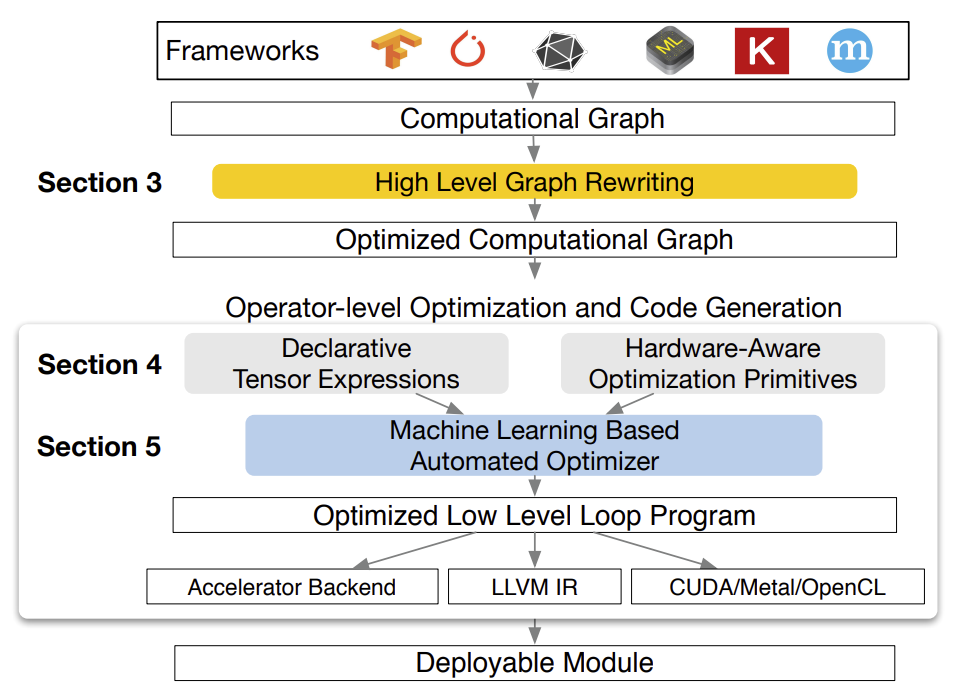
\includegraphics[width=8cm]{img/3.png}
	\bicaption{TVM架构图 \cite{DBLP:journals/corr/abs-1802-04799}}{System overview of TVM}
	\label{TVM架构图}
\end{figure}


\subsection{计算机视觉算法部署的实现与挑战}\label{计算机视觉算法部署的实现与挑战}
\subsubsection{传统视觉算法}\label{传统视觉算法}
传统计算机视觉的处理方法一般是多层次的,例如通过多个种类的算子进行滤波,获得不同的特征来做出决策。常见的包括颜色特征(颜色直方图),纹理特征(小波变换),形状特征(傅立叶形状描述符)等,最知名的还包括尺度不变特征(Scale Invariant Feature Transform,SIFT\cite{ng2003sift})等,其作为重要的特征算子,和传统的机器学习算法例如支持向量机SVM(Support Vector Machine)和分类算法KNN(K-Nearest Neighbors Algorithm)结合使用,广泛用于一些图像分类问题。这类算法对张量(Tensor)计算的专用硬件没有依赖,因此在系统角度而言,不涉及到硬件异构,产生的任务均可以视为一般的CPU负载,仅需要描述好数据之间的传递和依赖关系,就可以相对容易的调度。

\begin{figure}[htbp]
	\centering
	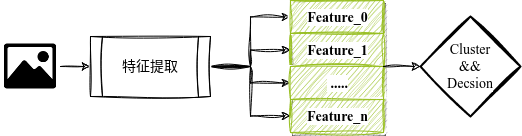
\includegraphics[width=8cm]{img/trad_vis.png}
	\bicaption{基于传统视觉算法的计算流程}{Computational flow of traditional vision algorithms}
	\label{基于传统视觉算法的计算流程}
\end{figure}

\subsubsection{推理部分}\label{推理部分}
当代深度学习算法,尤其是计算机视觉类算法,基本已经进化为一种端到端的模型(End-2-End), 不再需要手工设置特征提取和分类器等模块,以一整个深层模型,直接取代了传统算法的主体部分,并在分类,检测,分割,识别等一众任务中,精度指标相较传统算法取得显著优势。当前,工业领域应用最广泛的ResNet,YOLO,R-FCN等网络都体现出模型深层化的趋势,以ResNet50\cite{he2016deep}为例,其网络包含49个卷积层和1个全连接层,其总体参数超过两千万,整体计算量超过38亿FLOPs,整个运算过程如果单纯的放置在CPU一侧,将造成较大的计算延迟,无法满足实际业务场景的需求。

由于深度学习模型的推理和训练,其任务主要为密集的矩阵计算和梯度传播,重复度高,专用性强,且又因为应用广泛,具有较高的商业价值,因此厂商直接以ASIC(Application Specific Integrated Circuit)的形式,从底层硬件方面进行支持和优化,推出了专门用于AI计算的半导体芯片。其内部的电路结构可以执行特殊的指令集,相对于普通的CPU,极大的增加了带宽和处理器的个数,同时将单个处理器的结构进行简化,在降低成本的同时,能快速执行简化后的指令集。其在运算效率和计算成本上,都和使用CPU相比有显著的优势。大多数情况下,视觉算法的模型推理部分,会尽可能的放置在针对矩阵计算和梯度传播有专用硬件模块的芯片(NPU,GPU等)来运行,取得结果后再拷贝回CPU侧,调度原则不同于一般任务。

给部署阶段造成困难的还包括模型的持续迭代。计算机视觉算法是一个高速进步的领域,算法开发工程师经常需要推出新版本的模型。这种迭代一方面是来自于科学研究领域的不断进步,新的模型具有更高的准确率指标,或者是改进后只需要更少的参数,具有更优秀的推理延迟。另一方面则是由于视觉算法是基于有监督训练,其在上线的使用过程中,还会不断的收到来自用户或者自身团队提供的标注数据,这些数据会用于不断的扩充训练集,让模型具有更好的泛化能力和准确率。

虽然这一过程是在模型的生产环境完成,和部署过程属于独立的软件工程模块,按照开闭原则(Open-Closed Principle)仅需做到输入输出接口的一致性,即可让模型迭代和替换的过程独立。但实际的情况,新的模型在具体部署硬件上有支持差异。

例如基于于注意力机制的Transformer\cite{vaswani2017attention}模型,由于其前后数据依赖程度远低于循环神经网络RNN和长短时记忆网络LSTM,大幅度改进的并行性能以及良好的表示学习能力,使得其在自然语言处理领域取得了巨大的成功,并拓展到视觉领域,例如ViT(Vision Transformer)\cite{khan2022transformers}。虽然在训练侧得到实现,但部署方面,很长一段时间仅有官方训练框架直接生成的模型可用(例如PyTorch直接生产的Torch Script模型),缺乏对硬件支持优化。即便是生态最完善的英伟达,也花费了接近3年(2017年发表,2020年3月发布TensorRT7.2)才支持将常见的Transformer模型(BERT、GPT-2等)转换为TensorRT\cite{tensorrt7}可识别的格式。与此形成对比,华为直到昇腾AI异构计算架构CANN 6.0(2022年11月发布)\cite{HuaweiCANN},才首次支持\verb|torch.nn|的Transformer Layers算子。

无论是出于实际的经济成本,还是整个智能化软硬件的国产可控,目前有相当大比例的客户,在软件的集成采购中,会要求使用指定的品牌范围的硬件设备。这导致在推理部分的实现上,一个服务于相同请求的计算机视觉算法,可能同时使用多种不同的推理模型,运行在多种不同的硬件环境上。因而在部署开发的过程中,需要充分考虑到不同硬件混合的兼容性和模型替换需求,做好硬件负载和推理延迟的评估,防止使用参数量过大且缺乏优化的模型,尽量协调整个计算流水线的吞吐执行。

\subsubsection{前,后处理部分}\label{前,后处理部分}
工业化算法的部署场景需要更多的处理步骤,例如最常见的摄像头输入,传入图像往往有不同的尺寸和清晰度,除了传输过程中的解压缩和解编码,还包括一些根据后续算法定制化的额外操作。一个常见的例子是,经常作为提取特征的卷积神经网络ResNet,其输入需要大小为固定的$224\times224$,像素值经标准处理后在$[0, 1]$或$[-1, 1]$范围内的浮点数矩阵,因此输入之前需要使用填充(Padding)的方式,将输入图片缩放至一定尺寸,再将其嵌入到一个大的黑色图像中,使其能够适应ResNet的输入,或者也可以通过裁剪(Crop)将输入图片从中心裁剪为固定比例。这部分的计算称为数据的前处理(Pre-processing),属于端到端模型以外的范畴,对应在输入图像经过神经网络模型之前所进行的一系列操作。

常见前处理包含:
\begin{itemize}
	\item[$\bullet$]尺寸缩放(Resize):将输入图像调整为神经网络模型指定的大小,避免尺寸差异对模型性能的影响。
	\item[$\bullet$]归一化(Normalize):将图像像素值缩放到固定的范围内,如$[0,1]$或$[-1,1]$。
	\item[$\bullet$]色彩空间类型转换(Color Space Type Conversion):将图像从RGB(Red,Green,Blue)色彩空间转换为其他色彩空间,如灰度图像或HSV(Hue Saturation Value)色彩空间,可以更好地提取图像的特征。
	\item[$\bullet$]解码(Decode):对于一些视频和图像数据数据,传输的过程可能会按照一定的编码方式进行压缩,需要解码之后再进行处理。
\end{itemize}

和前处理形成对应,计算机视觉算法同样包含后处理过程。后处理(Post-process)通常是指对算法输出的结果进行一些加工和过滤,以得到更加准确和可靠的结果,相对前处理而言,后处理逻辑相对会更复杂。常见的后处理包括非极大值抑制(Non Maximum Suppression,NMS)\cite{bodla2017soft}、去重、后验概率校准等。例如,在目标检测算法中,算法输出的是一组候选框(Bounding Boxes),需要经过NMS算法去除高度重叠的框,并进行类别预测和后验概率校准,最终得到检测结果。人脸识别算法中,通常会对算法输出的人脸特征进行去重和归一化,以提高识别准确率。后处理的目的是提高算法的准确率、鲁棒性和速度,并适应不同的应用场景。

前,后处理是计算机视觉算法中非常重要的环节,可以极大地影响模型的性能和准确度。然而不同的算法需要进行不同的前,后处理操作,其实现方式非常多样化,常见的原因包括:
\paragraph{专用硬件支持}虽然前处理和后处理的运算并非完全如推理模型一样,表现为纯粹的张量运算,但其仍然会包含很多显著的并行优化点,其原因主要在于图像信号本身就被表示成矩阵形式,其处理天然符合一些线性代数的运算优化方法。现代图形芯片出于渲染管线(Render Pipeline)高并行度的计算任务需求,设计了大量的流处理器和高带宽,被逐渐拓展运用在一部分类似的通用计算环境。例如经典的图像处理库OpenCV\cite{bradski2000opencv},早在2010年就开始着手将传统图像处理的部分算法,包括常用的前处理和后处理,利用NVIDIA的CUDA\cite{sanders2010cuda}编程模型来实现。

长期以来,国内的计算芯片发展,一直面临如X86指令集这类的专利授权问题。ASIC芯片因为不需要考虑固有的软件生态,因此相对容易回避限制,被广泛视为产业自主化的机会之一。经过数年的发展,有类似于华为海思这样借助旧有芯片设计业务的入局者,也诞生了包括寒武纪,壁仞这类专精于此类芯片的创业公司,其整体呈现出多样化的趋势。相较于训练框架逐渐因为软件生态走向统一,专用的计算芯片没有兼容性的考虑,不同于GPU通常采用IEEE 754标准的浮点数运算,ASIC芯片以更强的专用性目的而实现,采用定点数运算、半精度浮点数运算或其他非标准来适应训练或者部署的场景,只需要能正确的执行模型,输出精度差距保持在一定范围内即可。

由于ASIC芯片设计的定制性太强,为了保证主要场景下的性能和效率,有时会限制芯片在其他任务上的可用性,难以像CUDA一样抽象出一套完整的并行计算框架。同样也因为开发时间较短的原因,软件生态和NVIDIA相比还有难以逾越的差距。前文所提到推理加速器TensorRT,支持以插件的形式,增加框架训练输出模型以外的额外部分,包括例如\verb|leaky relu|\cite{xu2015empirical}这样的网络层, 还可以以类似的形式将一部分前处理和后处理操作,封装到推理模型内部,得到通用优化,CUDA也可以直接编写运行在GPU上的并行程序,进行灵活的显存管理。

\begin{figure}[htbp]
	\centering
	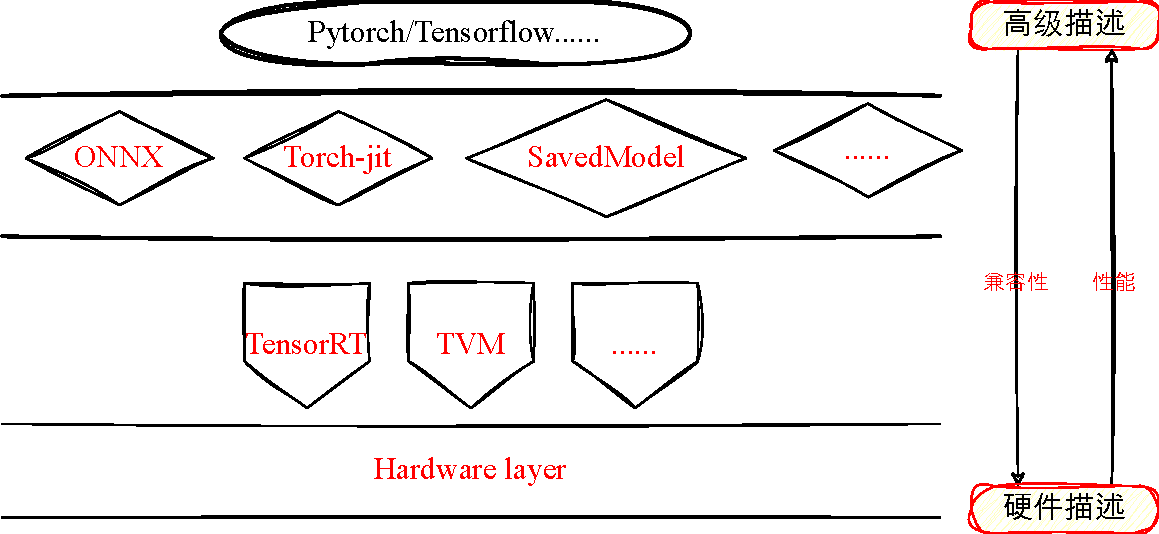
\includegraphics[width=8cm]{img/4.pdf}
	\bicaption{视觉算法模型的兼容性和性能权衡}{Compatibility and performance trade-off of vision algorithm model}
	\label{视觉算法模型的兼容性和性能权衡}
\end{figure}

而国内硬件设备在软件的完善程度参差不齐。一个具体的例子是,作者于2022年初进行华为ASCEND加速卡相关开发过程中,发现其专用的达芬奇架构固件只支持通过API的方式去调用一些固定算子,定制化的函数仅可通过组合实现,缺乏更加底层的接口,由此导致部分前处理,后处理的代码不能支持,仅能放置在CPU侧来运行,进而引发数据在ASIC芯片显存和通用内存之间来回拷贝的额外的开销,需要重新考虑调度安排。
\begin{figure}[htbp]
	\centering
	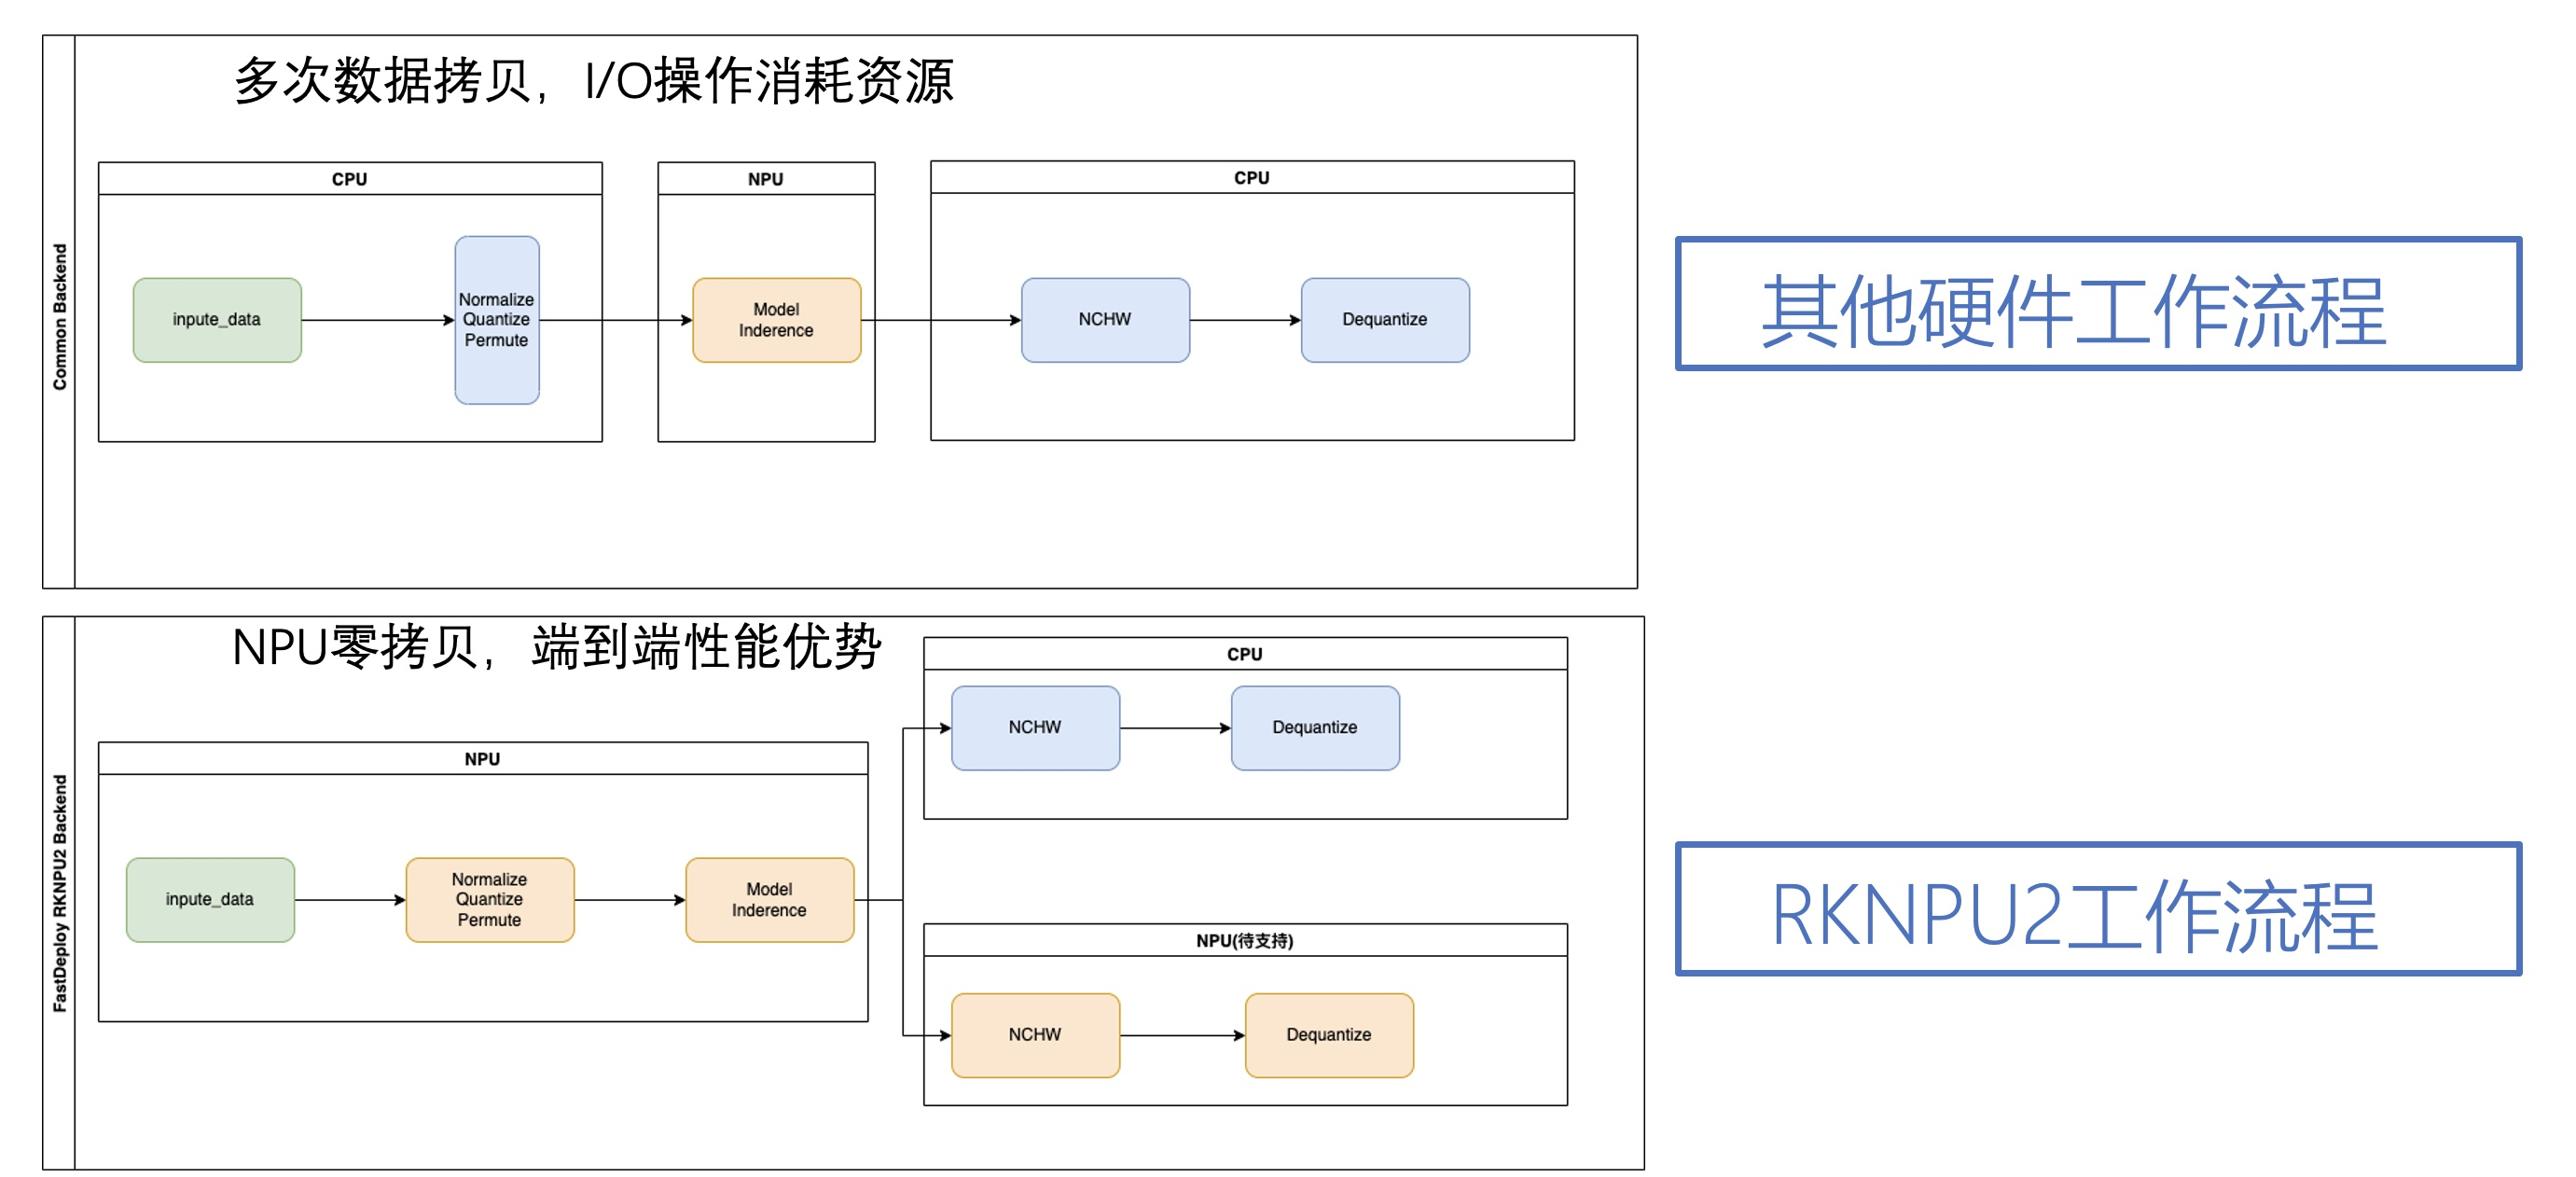
\includegraphics[width=8cm]{img/rknn_support.jpeg}
	\bicaption{RK芯片集成处理(目前暂无)\cite{rknnprocess}}{RK chip integrated processing(still not support)}
	\label{rknn-support}
\end{figure}

上述讨论说明,由于部署阶段既要贴近硬件的性能优化,又要满足多种硬件的适配,因此必然导致高度的软件封装,同一函数接口的执行开销难以评估,进一步影响到软件层面的实现和调度。
\paragraph{计算成本和开发难度}
相较于Intel最新的桌面级CPU-13900k,即便考虑AVX(Advanced Vector Extensions)512指令集的SIMD(Single Instruction Multiple Data)和FMA(Fused Multiply Add),其理论算力约为RTX4090的3$\%$($\geq$100TFLOPs),仅考虑单位算力成本,尽可能的去选择GPU是一个更合理的选择。然而在实际的应用场景中,CPU的主要功能远不止完成计算,而是执行更加多样性的活动。例如需要频繁中断的网络和IO(Input/Output)业务,常需要配置多核心来提高响应速度,主频则少有满载的情况,甚至普遍不足峰值10$\%$,生产实践中遇到的情况是,负载最高的硬件往往是专用的深度学习计算卡,CPU的一般并非性能的瓶颈所在,计算资源常有冗余。一般情况下,部署原则是尽可能使GPU,ASIC部分硬件达到最高的利用率,部分前处理,后处理的是否放置在GPU等设备上执行并不固定。

除去硬件考量,即便是有完善文档和调试工具链的CUDA,编写面向GPU的并行程序也对体系结构知识有一定门槛,软件工程师的开发难度同样需要考虑。一般的,对于不构成性能瓶颈,在总体延迟中占比较低的处理,会直接选择以CPU侧实现来节约开发人员的时间,对于通用性高,时间开销大的算子,会考虑针对具体的硬件去做特化的实现,以此来降低开发人员的实现难度,便于合作的和迅捷开发。

\subsection{计算机视觉算法的部署外环境}\label{计算机视觉算法模型的部署外环境}
上述内容讨论了计算机视觉算法部署过程中,在计算层面将整个推理过程进行封装,对外提供稳定的抽象功能接口(动态库,远程过程调用(Remote Procedure Call,RPC)),内部完成模型的加载和版本管理,并对不同的硬件支持进行实现过程,这种方式可以近似的表示为下图:

\begin{figure}[htbp]
	\centering
	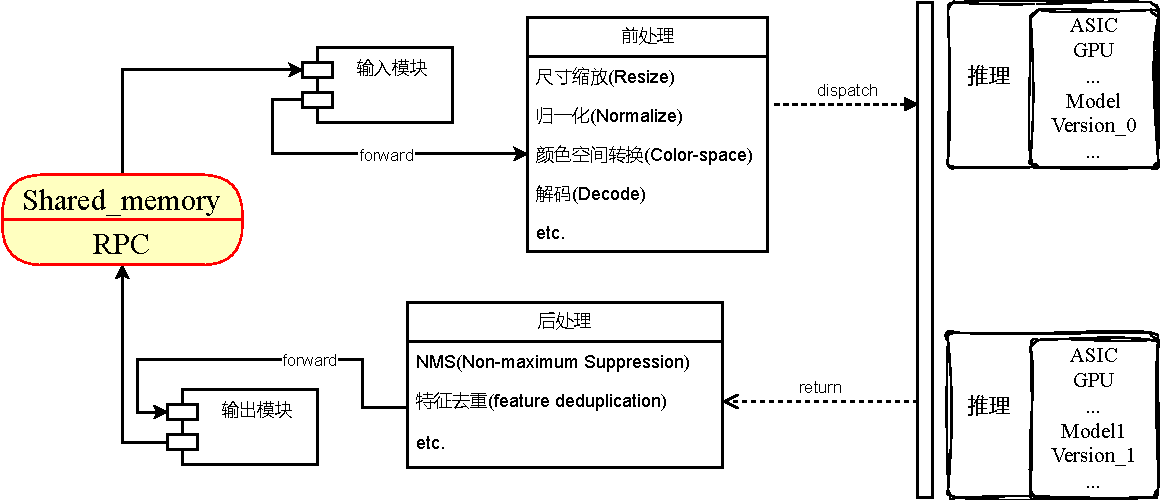
\includegraphics[width=8cm]{img/frame.pdf}
	\bicaption{计算机视觉算法部署框架}{Computer Vision Algorithm Deployment Framework}
	\label{计算机视觉算法部署框架}
\end{figure}

我们在此定义部署的外环境,指包含从数据输入到结果输出,除去纯粹计算部分以外的环节,即我们将整个推理侧视为一个完整的服务端来考察,如\ref{计算机视觉算法部署框架}所示,其部署的外环境包括软件本身的运行环境,以及数据的传输交互(输入输出模块)。

对基于深度学习的算法而言,一个成熟的落地场景是推荐系统,例如网络购物平台的商品推荐,或者内容平台的视频和文本推送。这一类型业务的特点是数据和计算硬件物理空间相近,处于同一数据中心,通常还有专用的传输线路。同时,对延迟的稳定性要求不高,更强调单位计算的成本更低和高并发下的可拓展性,外环境基本近似为基于虚拟化技术云计算平台。

实际场景中视觉算法更偏向于现场部署,用户基于成本考量,以及数据的安全问题,并不希望使用云服务。举例一个港口项目的情况,内部系统集成了集装箱破损检测,区域门禁,人员安全帽行为检测等多样化的业务。虽然功能多样,但并发量小,处的数据量规模低,大部分时间只执行有限种类的算法业务,出现复杂问题的概率不高。区域内一般有中心化的机房,数据的传输经由内网,通常会集中式的混合部署一些服务,比如简单的Web程序和数据库等。

一种更为广泛的情况则是基于边缘计算的部署,其主要目的是通过在用户或数据源的物理位置附近进行的计算,以此降低延迟,节省带宽。工业场景下的分类和检测,当任务相对复杂时,除去算法的实际功能指标外(Recall/Precision),通常还会对服务的质量提出较高的要求,例如可靠性和延迟响应速度。这种情况多见于安防和政府治理等领域,虽然其主观目的是提供可靠易用的智能化服务,但同时也必须考虑到数据安全和隐私保护的问题,因此一般不会长时间保存待分析数据。同样,嵌入式系统下硬件资源无法进行弹性拓展,使用缓存队列一类的组件保存待处理请求,需要控制在尽量小的规模以防止过度占用内存。

由于请求基于流式(Streaming)\cite{muthukrishnan2005data}处理和输出,这类系统并非完全强调实时性(Real Time)\cite{jaffe1990software},而是允许请求在一个小的窗口期内完成,即信息的输入,检测结果的输出之间可以有一段的窗口延迟。举例说明,跟踪高速行驶的车辆,并对其属性信息和特征(车辆的颜色,类型), 车牌号码等做出识别,同时甄别是否有违章行为,这个过程允许有一定的延迟,但会非常强调延迟的稳定性,因为流式处理下,请求积压后只能丢弃数据,可能导致应被监测的非法行为遗漏,以及统计信息丢失。

\begin{figure}[H]
	\centering
	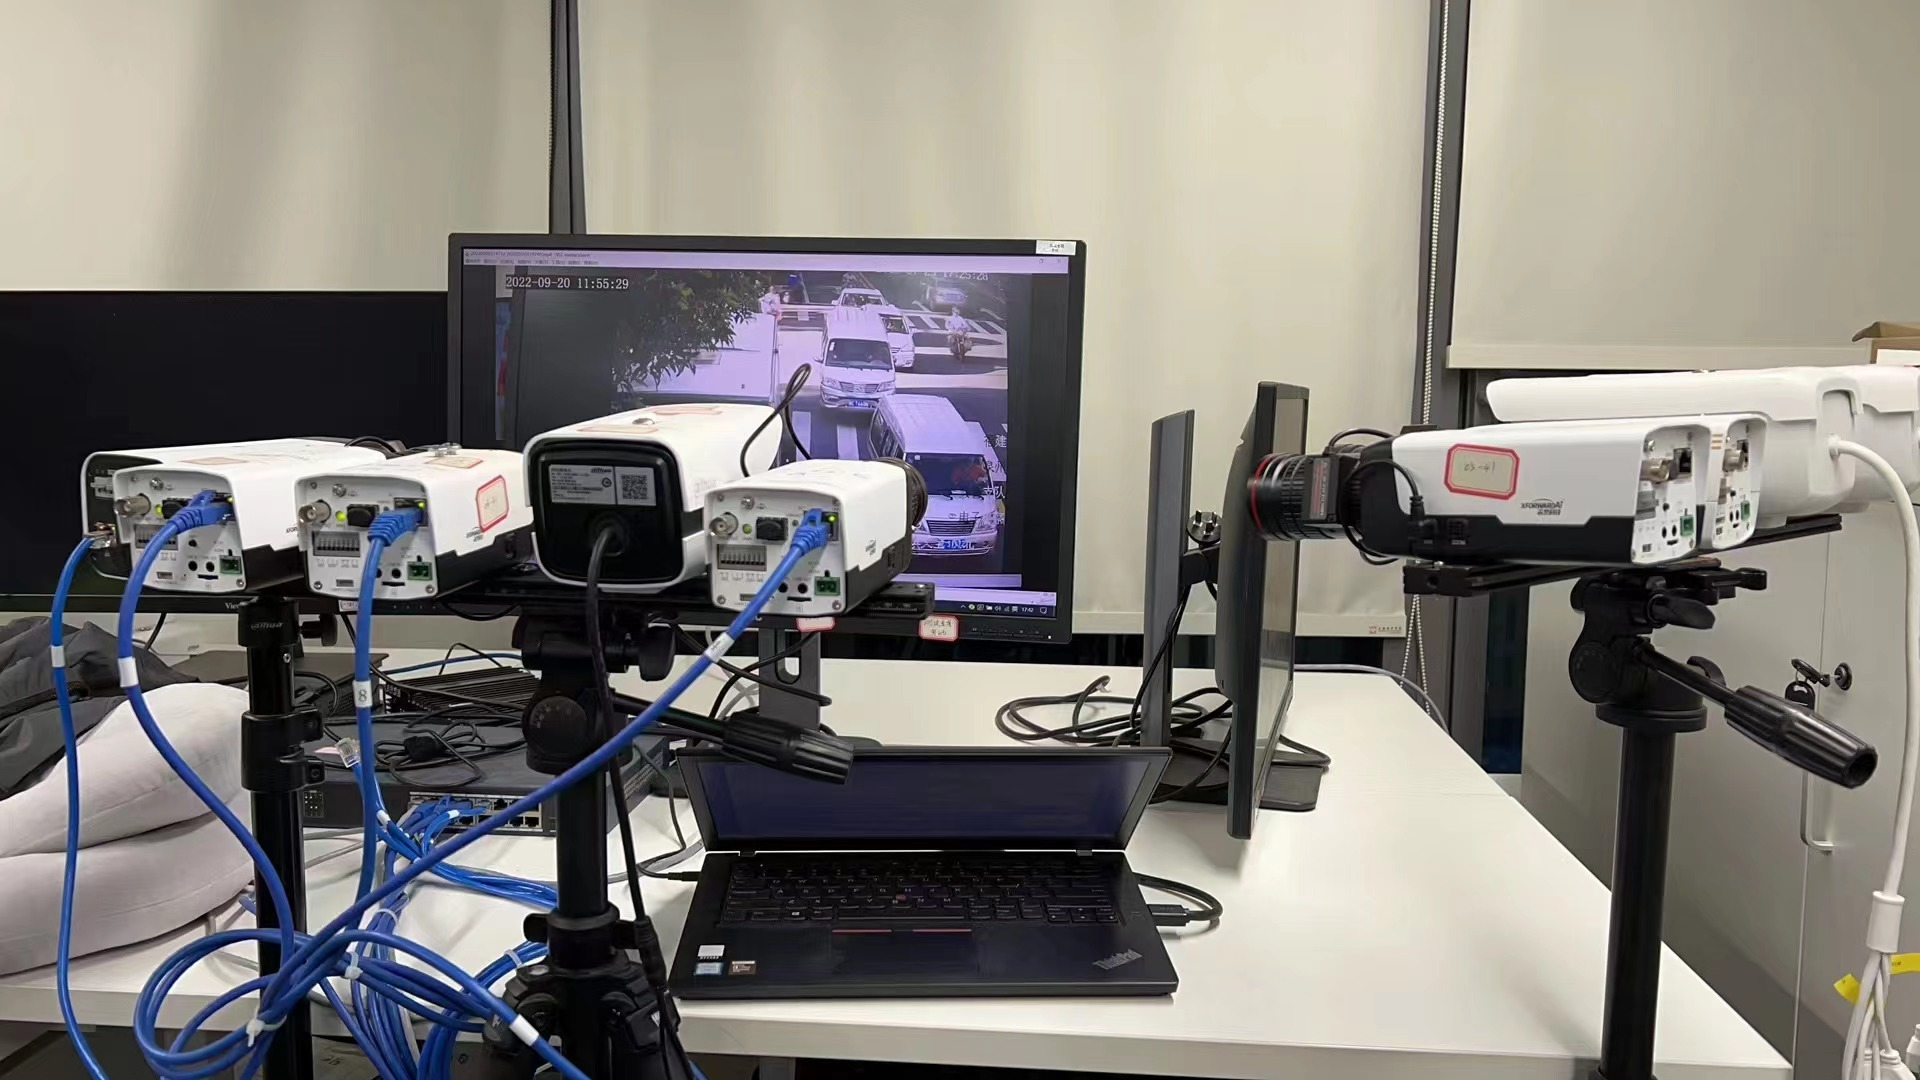
\includegraphics[width=8cm]{img/hd.jpeg}
	\bicaption{有线直连的超清摄像头(拍摄于实习公司)}{Ultra-clear camera with direct cable connection (taken in my intern company)}
	\label{有线直连的超清摄像头}
\end{figure}


下图描述了类似的架构场景,摄像头配置在道路的不同的位置,信号清晰度普通的低功耗摄像头,会被安装在交通信号的灯柱上,可以通过WIFI或者移动网络,将数据传输到本地的路由器。部分高功耗高分辨率的摄像头,则采用独立供电的方式,并通过高带宽的有线网络的形式传输到本地的路由器。路由器再将数据传输到边缘计算设备,多路聚合的视频信息会通过算法进行处理,运行面向车辆,驾驶员等目标的属性检测和行为识别算法,最终获取的信息会传入防火墙(网关)外的数据中心,做更进一步的服务处理。

\begin{figure}[H]
	\centering
	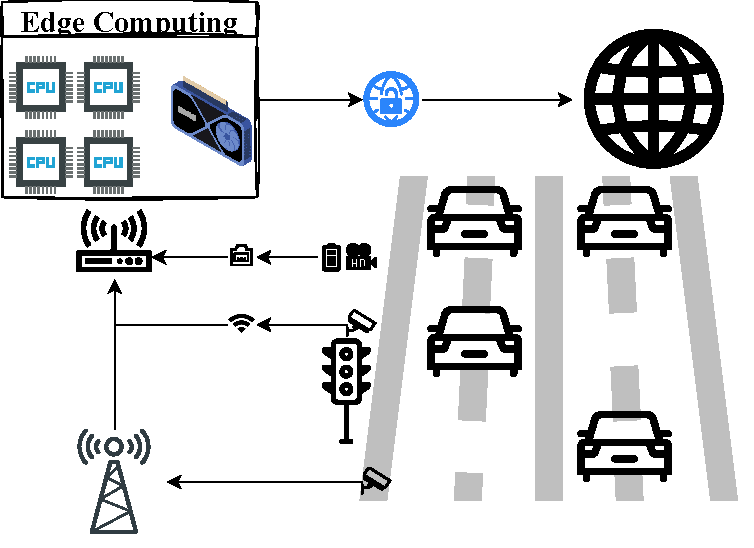
\includegraphics[width=8cm]{img/trafic.pdf}
	\bicaption{交通场景的边缘计算部署}{Edge Computing Deployment in Traffic Scenarios}
	\label{交通场景的边缘计算部署}
\end{figure}

参考上述示意图,不难发现,以边缘计算形式对计算机视觉算法进行部署,其整个运行的流程除去\ref{推理部分}描述的推理部分和\ref{前,后处理部分}的前,后处理部分以外,其整体延迟和可靠性还和传感器到计算硬件的传输过程有关。无线网络传输的延迟会因为传输距离,信号干扰,障碍物等原因增加,移动网络(5G)则容易因为用户数量突然增加而导致拥塞控制不当,进而引发传输问题。因为帧率和分辨率不同,各个图像传感器自身传输数据量也不同,这也会对延迟产生印象。即便我们将推理计算部分的封装视为绝对可靠,但由于计算机视觉算法的部署外环境,无法像虚拟化平台一样提供容错和备份能力,边缘计算硬件,网络,接口任一节点故障,都将影响整体服务质量。同时,区别于传统虚拟化服务器,边缘计算业务通常涉及数据安全和隐私保护,导致我们难以获取足够的运维信息,对故障进行快速的定位和考察。

\section{计算机视觉算法延迟观测的重要性}\label{计算机视觉算法延迟观测的重要性}
从算法工程师完成模型的参数调试,到部署为平稳运行的推理服务,不仅需要具体考虑软件,硬件的兼容性和复杂性,同时还涉及到工程成本的权衡,以及外环境稳定性等问题。了解各个步骤运行延迟,在整体运行过程中的占比,不仅可以作为优化指引,满足性能调试方面的需求,同时,面向一些对于稳定性和可靠性要求较高的,例如以流式视频输入的分类检测任务,也需要一些延迟方面的信息,对\ref{计算机视觉算法模型的部署外环境}里提及的外部部署环境故障进行事后跟踪和故障定位。

QOS(Quality of Service)可以用来衡量端对端服务的质量,传统意义上这一指标主要用于计算机网络中具有实时需求的业务,其用于评估任务是否能够以可接受的延迟,稳定响应请求的发起端。例如对于语音通信,视屏会议等应用场景,需要准确,快速的在服务端和客户端之间传递数据信息,以达到较好的信息交互体验。QOS的作用即为评估例如网络延迟,丢包具体会对服务的质量造成多大的影响,具体的,例如会对信息的完整度,卡顿,清晰度等进行量化的评估,进而作为应用程序在带宽分配,传输调度上的参考,以满足用户的需求。

计算机视觉算法的部署一般分为内部调试和外部发布两个开发阶段,内部调试主要以正确性验证为主,容许较为宽松的额外负荷,对外发布阶段则需要考虑性能,功耗等多方面的问题,对视觉算法这类延迟和资源受限的应用,尤其是部署在边缘计算硬件的情况下,还需要考虑系统运行具体环境,调整一些参数设置。由于正确性依赖于模型算法本身,因此如果想评估视觉算法的QOS,作为优化方面的参考,应当用响应时间,即延迟方面来进行衡量。

此外,对于部署的外环境下故障难以定位的问题,延迟的记录可以对计算机视觉算法的部署平台,给出一定的事后追踪能力。主要方法为在视觉算法运行过程中记录和延迟相关的日志,当出现故障或错误时,通过查看延迟及其相关的元信息来追踪故障的发生位置,有助于更好地了解系统的运行情况和发生的事件,提高系统可观测性与可靠性。

\section{计算机视觉算法延迟观测的一般方法与不足}\label{现有计算机视觉算法延迟观测的一般方法与不足}
对计算机视觉算法的延迟观测,至少应包含以下几个步骤:
\begin{itemize}
	\item[1]在算法的关键阶段(如网络传输,文件系统操作的IO事件,图像前,后处理,特征提取、分类、检测推理等)插入日志记录代码,记录节点时间戳和一些程序上下文。
	\item[2]通过将结束时间减去开始时间,计算每个阶段的耗时。这些延迟信息可以记录在日志文件中,也可以通过其他方式进行收集和处理。
	\item[3] 将收集到的延迟信息进行可视化和分析,或者输入算法获取一些指标作为评估参考。
\end{itemize}

从实现的角度,除去多样化的指标分析环节,可以将上述过程分为事件观测和日志记录两个阶段。

\subsection{延迟事件观测}\label{延迟事件观测}
传统的延迟事件观测,主要有硬件工具和代码注入日志两种方式

\paragraph{基于硬件支持的性能分析(Profiling)工具}

出于性能调试和观测的目的,硬件厂商会提供一些专用工具,来分析算法时延。例如NVIDIA的Nsight Compute\cite{yang2020hierarchical}就是其中一种,原理是借助硬件驱动使能,直接插入一个观测中间层,先通过CUPTI(CUDA Profiling Tools Interface)进行信息收集,然后利用可视化图标和图形界面呈现汇总结果。

\begin{figure}[htbp]
	\centering
	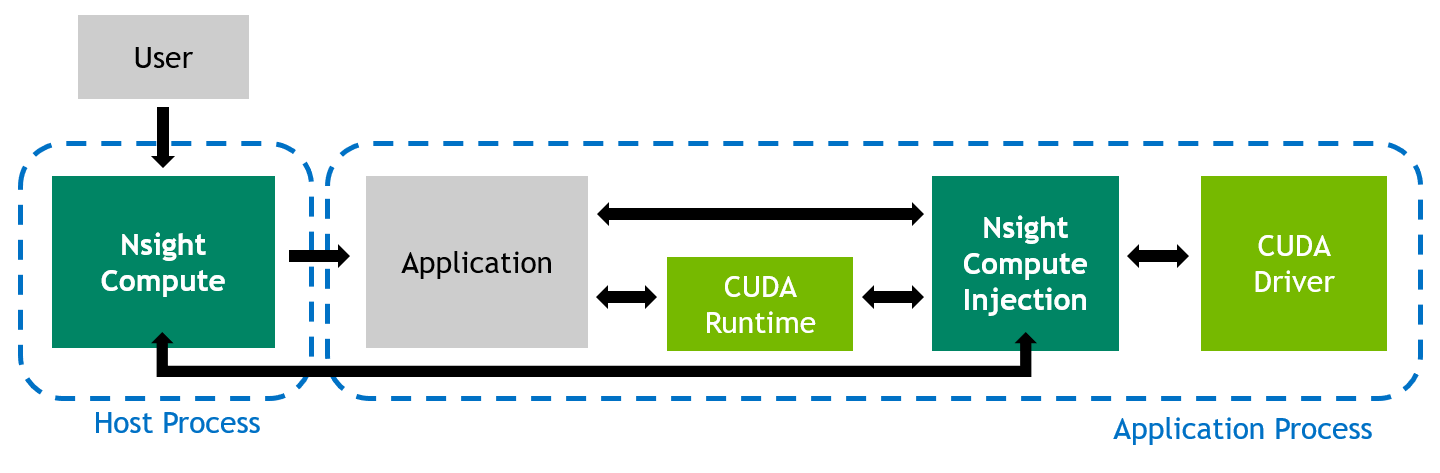
\includegraphics[width=8cm]{img/nsight.png}
	\bicaption{Nsight Compute的观测原理}{Observation principle of Nsight Compute}
	\label{NsightCompute的观测原理}
\end{figure}


这一做法的主要缺陷在于兼容性和局限性。兼容性主要体现在这一方法依赖于硬件厂商的软件支持,不适合需要部署国产ASIC芯片设备的混合部署场景。局限性体现在,工具对于性能观测的颗粒度缺乏定制性,对于运行阶段的时间划分是直接通过函数为单位,更适合开发者使用在发布前的调试分析阶段,查找整体的计算负载瓶颈。另外因为其捕获的信息颗粒度深入到指令集的层面,并且依赖于一套较为沉重的图形界面(Graphical User Interface,GUI),以嵌入式实时观测的角度来说,还存在性能负担过于严重的问题,一般更适合在云服务端的部署上使用。

\paragraph{基于代码注入的日志记录}
更加轻量级的做法,是在软件代码中嵌入日志记录程序,以字符串的形式记录时间和延迟情况,使用std::chrono库等C++时间函数,或Python中的time.time()等来获取时间戳,同时也可以定制化的去获取一些程序的元信息(例如上述CUDA Profiling API或者其他),例如:
\begin{lstlisting}[caption={使用CUDA Profiling API读取GPU状态信息},captionpos=b]
#include <cuda_runtime_api.h>
int device_id = 0;
cudaDeviceProp prop;
cudaGetDeviceProperties(&prop, device_id);
int gpu_utilization, memory_utilization;
cudaDeviceGetUtilizationRates(&gpu_utilization,\
&memory_utilization);
\end{lstlisting}

使用这种方式来记录延迟信息的缺点,首先是性能开销。作为一个运行时的延迟观测装置,我们希望记录时间的代价尽可能的低,而无论哪一种程序的时间函数,都依赖于系统调用。大多数情况下,日志信息还需要保留一些额外的元数据(Meta Data),例如CPU和GPU(ASIC)的运行时状态,内存占用,进程参数堆栈等,用于事后追踪时的故障定位,这些信息的获取过程同样依赖于系统调用,需要反复进行程序上下文切换(Context Switch)和从内核态(Kernel Space)读取到用户态(User Space)的数据复制。同时,在用户态生成字符串日志,需要首先需要通过参数填充(Parameter Handling),再从保存的数据中生成文本(Text Processing),这都会引入一些在嵌入式环境下不容忽视的性能开销,应尽量优化和避免。另一不足是这种文本生成方式,任何对日志产生过程的修改,都必须重新编译整个软件,维护难度较大,导致观测延迟为目的的注入部分与本身业务代码深度耦合,在软件工程的角度并不合理。

\subsection{延迟日志记录}\label{延迟日志记录}
延迟信息及其附属的元数据作为日志的形式写入,可能因为IO问题干扰正常的操作系统调度,因此将日志进程和软件任务本身分离,以提交(Commit)的方式,让日志进程独立完成记录持久化(Persistence),是一种常用的优化思路。在边缘计算的场景中,一个典型的设计就是基于发布-订阅模式(Publishers + Subscriber),即软件工程中的观测者模式(Observer Pattern)。通过集中式提交,构建专门的日志系统,还可以用来辅助系统调度。其所有的日志提交均通过基于网络的RPC接口,可以使用的框架包括Kafka\cite{kreps2011kafka}、RabbitMQ等,Kafka 侧重于高吞吐量而设计,而RabbitMQ偏向于更好的处理发布者和订阅者之间的复杂路由\cite{dobbelaere2017kafka}。


边缘计算设备,或是服务器中,以进程为单位运行的计算机视觉算法实例,作为日志发布者(Publishers),统一向作为订阅者(Subscriber)的日志进程提交产生的事件信息。这种模式的优越性在于具有很强的解耦性,边缘设备和独立运行的计算机视觉算法实例,启动后可以随时注册到日志进程中,只需确定好提交的方式,无需对日志系统进行修改,各自独立操作,同时系统可以采用分布式消息队列等方式来保证传输过程的可靠性,避免信息丢失或重复传递等问题。订阅者通过处理和分析日志信息,帮助管理者监控和调试边缘设备,了解系统运行状态,以此提高边缘计算的可靠性和稳定性。但缺点也非常显著,即网络消息传递的开销增加了带宽压力,并且中心化的日志接收节点需要显式的管理,造成了一定的运维难度,并且在部分性能要求较高的场景下,
分布式框架显然过于沉重。

\begin{figure}[htbp]
	\centering
	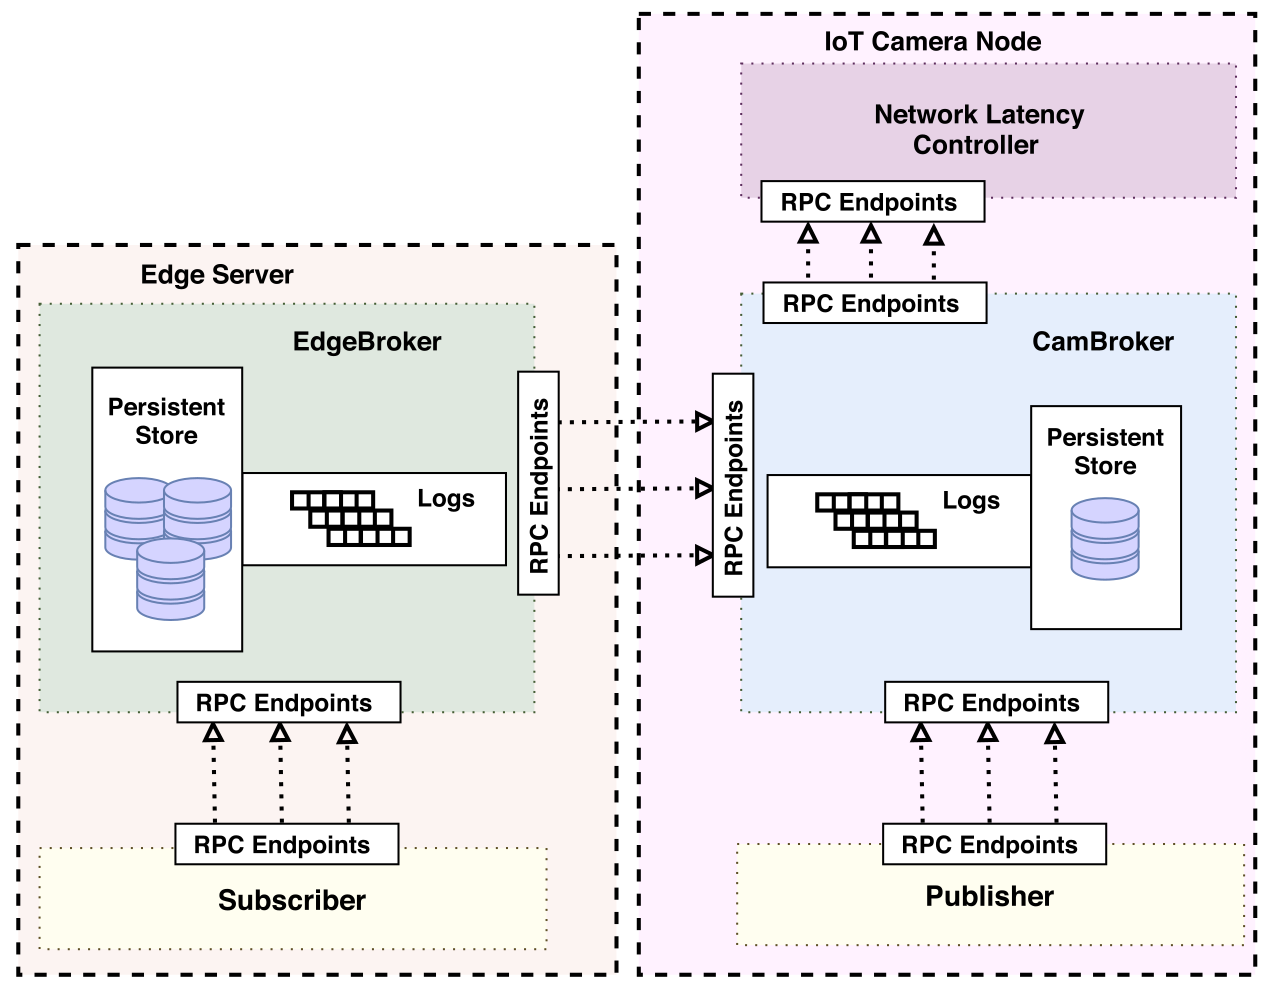
\includegraphics[width=8cm]{img/rpc_log.png}
	\bicaption{基于发布订阅的边缘计算日志系统\cite{george2021mez}}{Edge computing log system based on publishers + subscriber}
	\label{基于发布订阅的边缘计算日志系统}
\end{figure}

此外,日志写入无论是集中式还是独立进行,写入文件或发送到远程服务器的操作都无法避免,尤其是在IO速度较慢的嵌入式系统中,可能会导致服务整体的响应速度变慢。一些日志系统支持通过事件级别过滤的方式,只记录重要的日志信息,并采用缓存机制,通过批量记录减少IO操作次数,提高系统的IO效率。也包括使用异步处理,避免IO操作阻塞主线程或进程的执行。在嵌入式系统中这类资源受限的环境下,实现以上操作时,还需要注意减少软件依赖,控制程序体积。总体而言,延迟日志的记录部分,不仅需要进行充分的性能优化,还需要处理好与其他模块之间的功能衔接,往往需要针对业务场景深度定制。

\section{论文研究内容和创新点}\label{论文研究内容和创新点}
\subsection{论文研究的出发点}\label{论文研究的出发点}
本文研究源自公司业务实践中的需求,同时受到开源社区的启发。在计算机视觉算法落地部署的开发过程中,由于公安政府,工厂等客户需求各有侧重,并且需要同时针对寒武纪,华为,英伟达等不同的底层硬件,抽象出统一的接口,进行兼容和封装测试,以网络服务或者静态库依赖的方式,提供给更上层的业务框架来进行调用,经常需要进行各类不同目的的优化,甚至有时优化的主要目标是节约异构部分的硬件成本(减少ASIC和GPU的用量),这在传统信息服务中是不可想象的。

在这一过程中,延迟数据作为一个重要的优化参考,需要在每次测试中反复采集。基于传统方式的延迟事件观测,体现出了较大的局限性,在观测能力,观测维度,观测灵活性等各方面均有显著不足,且日志格式不统一,难以进行可视化。在此过程中,意识到视觉算法的部署SDK(Software Development Kit)缺乏独立的可观测模块,开始着手实现相关功能。

考虑到实际项目中,经常发生维护工程师远赴现场,结果只是简单的接口故障或者网络问题。因此也希望这种可观测性能满足一些边缘计算"盒子"在使用过程中的故障定位和事后追踪能力。

在对开源社区寻求解决参考的过程中,发现单纯引入一个更高性能的日志记录器,并无法解决部署环节复杂的延迟观测需求。而一种应用在无人驾驶领域,基于动态观测技术的定制化方法\cite{bpfgpu}则给予了思路启发,由此实现了一个基于内核BPF(Berkeley Packet Filter)\cite{mccanne1993bsd},和业务系统深度融合的轻量延迟观测系统。
\subsection{论文的主要内容}\label{论文的主要内容}
论文聚焦于计算机视觉算法延迟观测这一具体需求,具体讨论了如何在部署流程相对成熟的,2D识别,检测,分割这类业务时,面对复杂的部署条件,尤其是在边缘计算的场景下,以较低的代价,获取数据在各个环节的执行延迟,并拓展观测到一些常规运维工具无法获得,或者获取成本较高的底层状态数据。同时,也分析了这些数据在嵌入式系统中如何以尽可能低的代价存储,避免影响业务代码运行。

论文的主要内容即探讨了这一轻量延迟观测系统的技术选型和实现细节,基于绝大多数视觉算法部署,都会运行在Linux系统的客观事实,论文的设计以放弃对早期操作系统版本的兼容为代价,全面采用Kernel5.8(发布于2020年)\cite{bpfring}之后的新特性,换取适合嵌入式系统的低依赖和高性能。通过将BPF的用户态插桩技术,运用到计算机视觉算法模块化封装的实现中,借助对操作系统动态观测能力的二次开发,极大拓展了SDK的观测自由度,大幅度降低了延迟观测所需的工作量,并给出了面对不同硬件软件条件下,如何处理兼容问题的解决参考。

同时,论文还实现一个延迟信息专用的,独立的轻量级日志系统,进一步完善了整个工具的可用性。此处充分利用了内核原生异步IO(IO- URING)\cite{axboe2019efficient}提高性能。同时充分考虑了延迟信息的具体特点,通过设计定制化的存储格式,引入前置过滤的运行时算法,实现了对延迟记录过程中的性能优化,也让数据更便于后续的分析和使用。

进一步的,论文通过设计仿真实验,讨论了这一观测系统所捕获的持久化日志,如何在计算机视觉算法任务场景中得到应用。通过对基于计算图的计算机视觉算法部署方式进行模拟,在最新的国产ASIC芯片上,实践了利用延迟数据作为部署优化的参考信息的具体流程,以及故障后,运用延迟数据进行简单事后追踪的功能测试。

\subsection{论文的创新点}\label{论文的创新点}
论文的主要创新点在于,给出了在基于计算图-模块封装的计算机视觉算法部署框架下,如何引入内核动态观测的实现方案,并从原理上对性能优化和功能实现进行了细节讨论。同时,对于不同的硬件差异化的软件生态下,给出对兼容问题的一种解决参考。此外,还设计了根据延迟数据的具体特点,结合算法运行流程,生成固定格式延迟信息日志的方式,并在嵌入式系统的场景下进行了深入优化,以上为论文对应发明专利的主要内容\cite{patent}。

后续在工程实践中的结果表明,和现有的延迟观测方式相比,基于内核特性实现的方案,具有显著的性能优势和观测能见度优势,使用方式也非常灵活,经过简单的二次开发,就可以极大减轻延迟测量评估的工作难度。还可用于离线部署条件下,对一些简单的事后故障进行分析和定位。对此,论文设计了一部分仿真实验,不同于大部分视觉算法相关论文选择NVIDIA平台,本文选择在国产硬件,并且是最新一代的硬件平台上进行了测试。

同时由于本文的所实现的轻量级日志记录模块,不依赖于任何第三方库,仅需要高版本的内核支持,二次开发较为方便。也因本身和观测事件的生成框架之间是松耦合的设计,且实现的前置过滤模块对常用的延迟分布都具有一定的适用性,因此独立拆分后,完全可以作为一个后端框架去衔接其他延迟观测的提交结果。由此拓展实现的IO延迟观测的工具,还作为一个雏形项目,贡献到华为OpenEuler的开源社区中\cite{stortrace}。

\subsection{论文组织结构}\label{论文组织结构}
论文主要内容分为以下四个章节
\begin{itemize}
	\item[1]\textbf{绪论} : 研究的背景和意义,简要叙述了计算机视觉算法的工业部署流程,以及目前尤其是在边缘计算场景下,算法可观测性缺乏的现状和延迟的观测意义。
	\item[2]\textbf{计算机视觉算法的延迟观测} : 研究项目的设计和原理,叙述需求提出与分解过程,以及技术选型思路。
	\item[3]\textbf{轻量级视觉算法部署延迟观测系统实现} : 研究项目的工程实现,对这一轻量级延迟观测工具的实现要点和创新做了详细描述。
	\item[4]\textbf{边缘计算场景下的延迟观测实践} : 研究项目的实验仿真,通过一个简化的部署场景,展示了工具的特点和适用范围。
\end{itemize}



\chapter{计算机视觉算法的延迟观测}\label{计算机视觉算法的延迟观测}
\section{计算机视觉算法的运行时延}\label{计算机视觉算法的运行时延}

\subsection{基于计算图的模块抽象}\label{基于计算图的模块抽象}
计算机视觉算法的工业化部署中,一种主流的实现方式是模块化(Modular)之后构造计算图,具体做法是将计算机视觉算法分解为多个任务\cite{arora1998thread},然后使用任务图将这些任务组织起来,以便进行并行处理。任务图是一种有向无环图,每个节点表示一个任务,边表示任务之间的依赖关系。任务图的节点可以在不同的处理器上并行执行,以提高算法的运行效率。处于同一个进程地址空间内的计算,可以使用共享内存的方式来同步计算结果\cite{augonnet2009starpu}。当需要处理不同地址空间的处理器,甚至是异构系统(Heterogeneous System)时,则通过消息传递的方式进行通信,这种实现方式需要通常使用一些网络信息传递框架(RPC)。例如地平线公司的天工开物SDK,百度的PaddlePaddle\cite{ma2019paddlepaddle}部署部分,都采用了类似的方式来实现计算机算法的封装。

\begin{figure}[htbp]
	\centering
	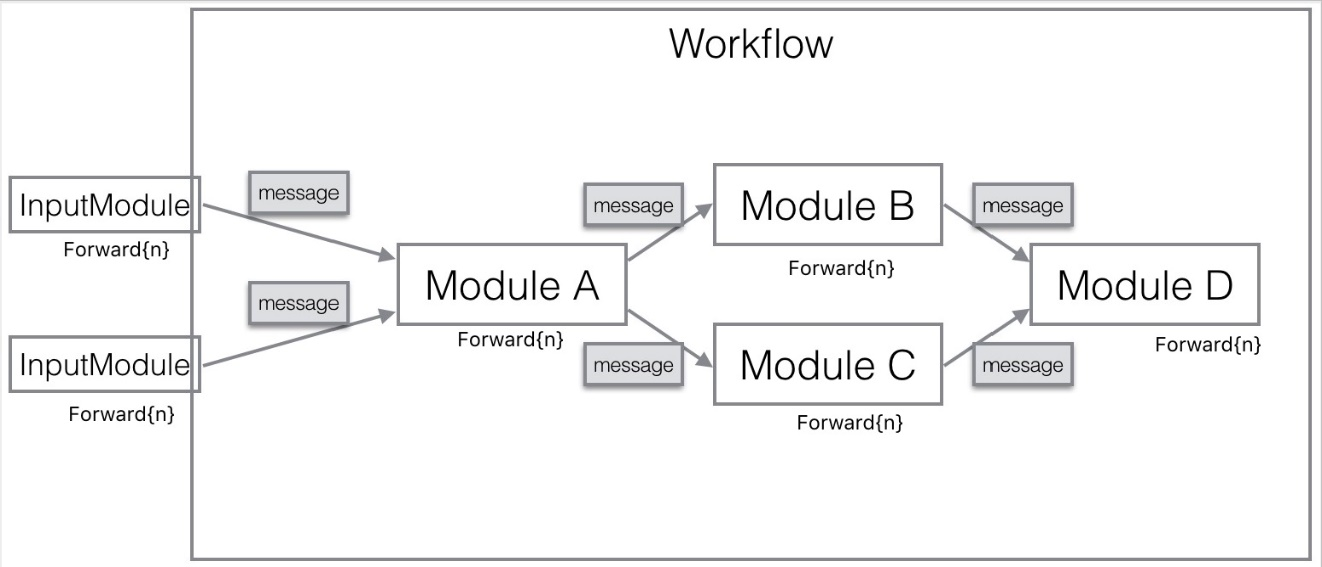
\includegraphics[width=8cm]{img/workflow.png}
	\bicaption{基于模块构造工作流}{Workflow based on module construction}
	\label{基于模块构造工作流}
\end{figure}

基于深度学习的视觉算法,其计算部分流程可以概括为前处理、模型推理和后处理三个阶段。前处理阶段通常包括图像缩放、归一化、裁剪、色彩空间转换等,这些操作需要以图像数据为输入,输出符合模型接口要求的张量数据,根据设计定位,可以封装为算子(Operator),也可以封装为计算图中的一个模块节点(Module)\ref{模块的基本结构}。后处理阶段通常包括后验概率转换、非极大值抑制、边框回归、关键点检测等操作,用于进一步优化模型的结果,这些操作也通常可以实现为计算图中的模块。

模型推理阶段是计算图中的核心部分,内部包括卷积、池化、全连接等多种结构,以及激活函数、归一化、Dropout\cite{srivastava2014dropout}等,每个节点都接受上一层的输出作为输入,输出结果经过下一层的处理,最终得到模型的分类或回归结果。但在模型的部署阶段,我们一般只会把模型作为一个端到端的模块来考虑,关注其吞吐量和计算延迟,而不会过度探索其内部的细节。

需要注意的是,用于推理计算的模块不一定只有一个,真实的业务部署场景下多个推理模型同时运行的情况非常常见,对于同种推理则会通过构造批次处理(Batch Forward)\cite{mcclelland1987parallel}以达到GPU(ASIC)的计算和带宽上限。此外,虽然专用硬件非常适合这一计算任务,少量情况下也会选择在CPU上运行。

完整考虑\ref{计算机视觉算法模型的部署外环境}描述的部署外环境,模块的抽象还应该纳入IO部分。常见的IO模块一般用来处理传感器设备的数据收发,例如不同的实例化IO模块和各种规格设备的摄像机,磁盘设备,网络套接字一一对应,生成具体的节点。无论作为输入还是输出,虽然没有具体的计算任务,但仍然需要进行完整的操作执行,因此同样应该提供对应的时间戳信息和附属的元信息。模块并不一定由单一的进程启动,例如负责发送数据的IO模块(负责管理某一相机设备的输入数据),完全可以单独运行,通过RPC的网络数据传输和计算图的其他节点通讯,基于这个前提,模块之间的信息同步可能涉及多种实现语言(Python,C++,etc.)和多个进程地址空间。

\begin{figure}[htbp]
	\centering
	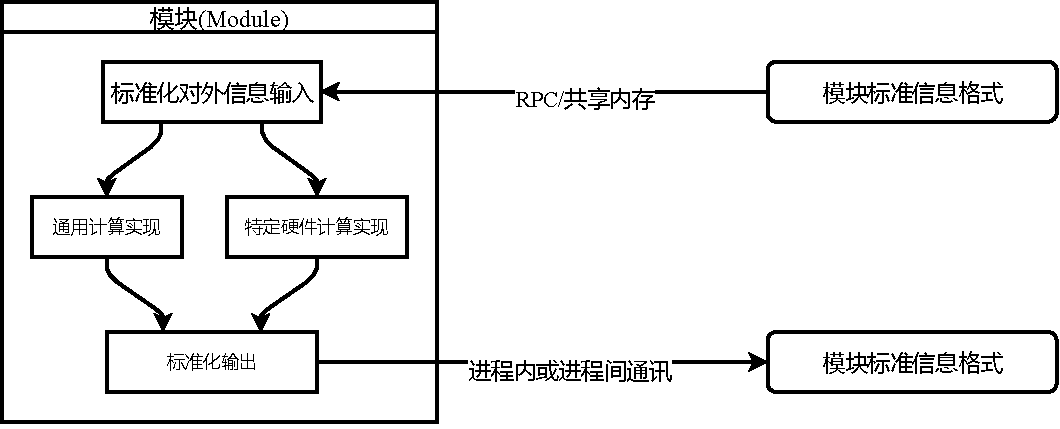
\includegraphics[width=8cm]{img/module.pdf}
	\bicaption{模块的基本结构}{The basic structure of the module}
	\label{模块的基本结构}
\end{figure}


\subsection{计算机视觉算法的部署延迟测量}\label{lantms}
\subsubsection{计算机视觉算法延迟的提取方式}\label{计算机视觉算法延迟的提取方式}
计算机视觉算法的部署延迟,通常是指从输入图像/视频,到算法产生输出结果所需的时间。当以计算图的模块为单位,对整个算法执行过程中做出抽象的过程中,整个流程的调用关系已经确定。这意味着对延迟的测量并非只能和传统的服务端相同,粗略的计算端到端的时间开销,而是可以针对整个完整的计算机视觉算法运行流程,逐环节拆分为单步延迟,以此来提供整体的观测能见度。

计算机视觉算法模块之间一般根据功能特点切分,但和一般基于CPU的计算任务不同,不同节点之间,尤其是负责模型推理的模块,其工作负载明显超出一个数量级。如果对整体时延求和,则推理模块的权重占比过高,导致其他模块的性能优化点不易发现。推理延迟的具体数值取决于使用的算法和实际的硬件设备。一般来说,现代GPU上执行一个PyTorch直接生成的Torch Script模型,中等参数规模(例如RetinaNet\cite{lin2017focal})的视觉算法模型,推理延迟大致在几十个毫秒。经过TensorRT的量化(Quantization),可以实现在精度下降个位数百分点的范围内,减少超过50$\%$的推理延迟,而单个前,后处理算子,基本在1-2ms的左右。但对于算子细节的实现优化并非没有意义,因为对于计算机视觉算法的部署而言,每一个算子都属于需要持续重复执行的热点路径(Hot Path),如何对这些常用计算函数的效率进行优化,也是学术界一直讨论课题\cite{cai2019maxpoolnms}。

而基于编译器层提供的性能观测工具(Nsight Compute,Intel VTune\cite{reinders2005vtune}),其切分的粒度一般以函数为单位,依赖于函数的符号表(Symbol Table),通过火焰图(Flame Graph)\cite{gregg2016flame}等方式进行可视化分析,帮助程序的使用者查找程序的性能瓶颈。这种方式的缺点在于颗粒度太小,如果以函数为单位,触发延迟信息记录的事件将会非常频繁,实时观测的开销太高,资源不足的情况下会影响算法本身的服务质量。
\begin{figure}[htbp]
	\centering
	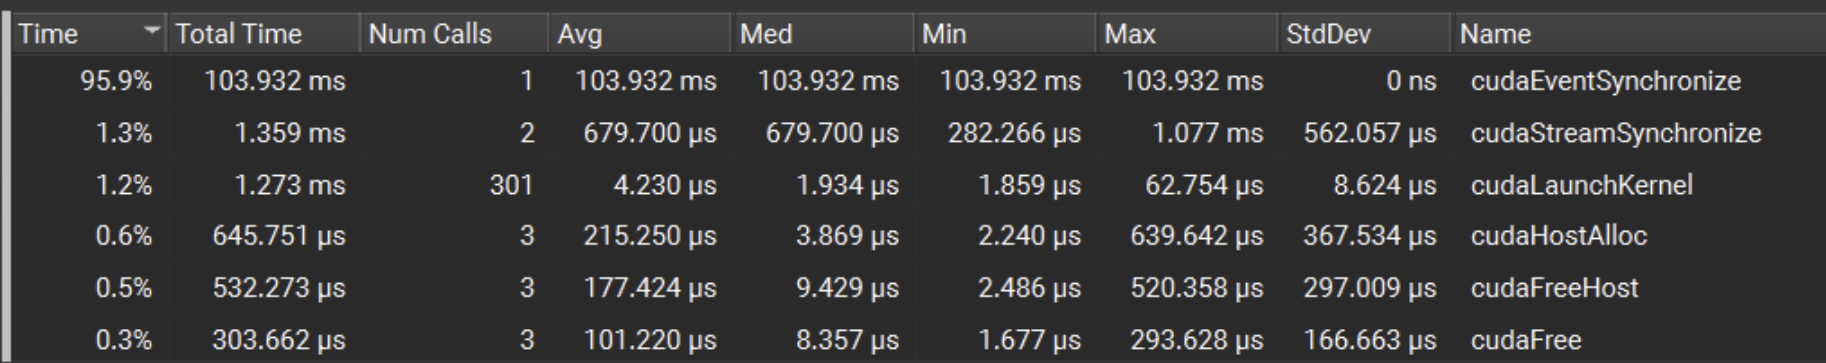
\includegraphics[width=8cm]{img/nsight_func.png}
	\bicaption{Nsight Compute的观测结果:颗粒度依赖于函数符号}{
		Nsight Compute Observations: Granularity Depends on Function Symbol}
	\label{NsightCompute的观测结果}
\end{figure}


因此,论文设计了一种基于阶段(Stage)选择的算法延迟测量方式,既考虑到观测颗粒度,也权衡了实时观测系统的低负载需求。具体的,以模块为时间戳获取的最小单位,一个阶段内可以放置多个模块。一个阶段至少需要在首个模块的进入点,和最后一个模块的结束点,触发延迟的记录事件,捕获时间戳和上下文信息,并提交到专用的日志记录工具\ref{论文观测机制示意图图例}。

一般的场景下,对于由多个视觉算法组成的业务模型,数据所需要经过的环节和顺序都是固定的,其运行的整个流程具有一个树形的拓扑结构。选择一个观测的阶段,首先需要对整个数据运行路径进行划分,由于整体是一个有向无环图,因此选择的阶段可能以多个分支结束,也可能是无分叉的连续模块。对于一段无分支的区间,可以任意选择连续的模块构造一个或多个阶段,当一个区间存在分支,由于我们一般认为,同一个模块处理的计算任务是等价的(近似于无状态函数,数据处理的开销和数据的来源无关),因此对重合的路径,应该切分处理,具体的,即一个阶段的选择,不能跨越产生分支的节点(可以作为端点),而应该将阶段拆分为分叉前后两份部分,重新在后续路径上构造新的阶段。

\begin{figure}[htbp]
	\centering
	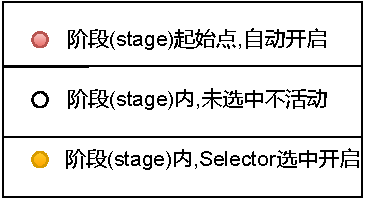
\includegraphics[width=8cm]{img/trace_l.pdf}
	\bicaption{论文观测机制示意图图例}{Schematic illustration of the observation mechanism in this thesis}
	\label{论文观测机制示意图图例}
\end{figure}

\begin{figure}[htbp]
	\centering
	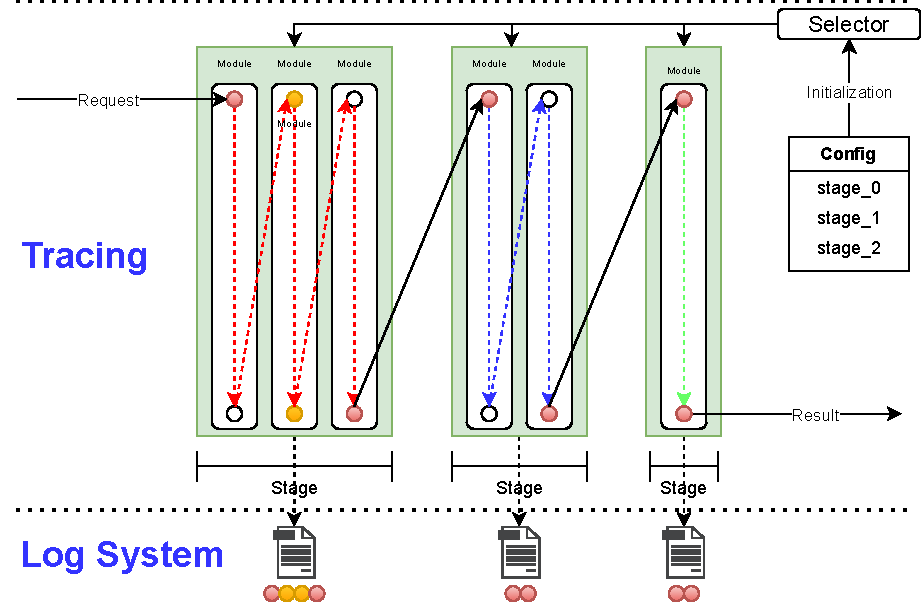
\includegraphics[width=12cm]{img/trace.pdf}
	\bicaption{论文观测机制示意图}{Schematic diagram of the observation mechanism in this thesis}
	\label{论文观测机制示意图}
\end{figure}

最终对于延迟提取方式的描述,是一系列以阶段为分区的延迟数据采集关系,这种构造过程无需修改代码本身,而是通过外部的配置文件(Config)。系统运行之前,会先实例化一个选择器(Selector),选择器通过读取配置文件的信息,确定阶段的划分方式,然后启动阶段两段模块上的内部设置为开启的观测点。这一机制依赖于操作系统内核的动态观测技术,具体实现在\ref{动态追踪技术概述}环节会详细讨论。但可以概括为,在每个模块的出,入口上放置的观测节点,是通过选择器(Selector)的启动后才具有触发延迟记录事件的功能,否则仅相当于一条不产生作用的空指令,不会导致额外的性能开销。

每一个阶段的延迟会被归档记录到一个日志中\ref{论文观测机制示意图}。对于单个模块,则开启和结束时间时间戳的差值就是模块的执行延迟,而到达下一个模块开启之前的时间,则可以视为调度和模块间的通讯延迟。这种情况下,不一定要选择阶段中全部的采样点,例如同一个进程地址空间之内的小计算模块之间的通讯和调度,大部分时候都没有观测的必要。


通过这一方式,可以灵活的控制观测的颗粒度,获取数据的详细程度取决于具体的需求。在软件的优化阶段,可以只选择前处理,后处理等部分等模块,避免推理模块的时延占比过高,不利于具体发现可以优化的节点。对比优化后的结果,可以只选择单一模块即可。运行时,延迟主要是用于事后的故障追踪,此时更多关注的硬件的情况,以外部传输,CPU侧,GPU(ASIC)侧来做大颗粒度划分,运行在同一硬件的连续模块直接归档到同一个阶段,减少产生的日志事件,降低观测的性能开销。

设计这种阶段选择的模式,实际生产中一个极大的便利点在于解除了业务软件本身和观测延迟部分的耦合,因为这种通过选择器去开启观测点的使用方式,并不会对软件目标运行产生影响,换而言之,采样和分析不会让被观测的对象所感知。这种方式构造了一种“热插拔”和“低耦合”,即采样和分析的工具是完全独立于生产系统,工具何时进行采样,何时和怎样进行统计分析,取决于工具的开发者和使用者。这使得测试不同模块的性能,只需要修改生成观测选择的配置文件,而不需要类似注入日志的方式,即使仅调整输出格式都需要直接重新修改和编译业务代码本身。并且“按需采集”的方式使得观测对于软件的性能负载可以调节和控制,一种机制即可适配运行时和发布前不同的延迟观测需求。

\subsubsection{计算机视觉算法部署中的延迟元数据}\label{计算机视觉算法部署中的延迟元数据}
\paragraph{延迟相关元数据}
当模块中的采样点触发延迟观测事件,获得此时时间戳时,当前程序的状态信息,即论文所定义的延迟元数据。元数据通常被定义为描述数据的数据,对于延迟而言,即一些和延迟相关硬件状态和软件状态。

模块是一种对于底层实现的抽象,而硬件状态则指的是实际执行这一模块的物理环境,例如CPU/GPU/ASIC(Neural Network Processing Unit,NPU)的工作状态。以CPU侧的运行为例,一般包括内存占用(Memory Usage),CPU当前频率,当前CPU上等待执行的队列长度等信息。而对于负责神经网络推理,和部分特殊的前后处理计算的专用硬件(GPU/NPU)而言,由于其实现的体系结构非常多样化,其观测的指标更多取决于硬件驱动直接提供的定量评估值,例如设备利用率,显存占用等。部分嵌入式环境下运行的硬件还会提供一些特殊的状态信息来辅助调试,例如NPU部分的电压值,常用于功耗分析和故障调试等场景。

软件状态信息则主要包括程序的上下文,一般包括程序当前所属的进程、线程ID,以及一些运行时产生的变量,一般还会根据需求,选择函数的参数堆栈,调用栈信息等。如何利用这些信息相当自由,甚至于可以根据一些特殊需求生成一些额外的信息。

这些额外信息是衡量可靠性的关键参考,获取元数据的能力,是观测系统中能见度的直观体现。本文拓展计算机视觉算法可观测维度的方式,就是利用软件的状态信息去制作延迟数据之间的钩子(Hook),而事后追踪的故障定位,也非常依赖于这些元数据信息。
\paragraph{使用元数据拓展观测维度}\label{使用元数据拓展观测维度}
一般的服务端的观测工具,主要关注单一维度分析。例如最常见的是系统负载观测程序。举例iostat\cite{chandran2014monitoring},主要用于监控系统设备的IO负载情况,用户可以通过指定统计的次数和时间来获得所需的统计信息,类似平均请求扇区的大小,平均请求队列的长度,每秒读/写的扇区数(rsec/wsec)等。这种观测一般仅限某个单独的维度,具体来说,这种观测类似于对系统运行某一个环节,进行横向的截面采样,统计的指标一般是同类数值的平均值/最大值/最小值等分布信息。

一部分原因是因为这些工具诞生于早期的UNIX,设计核心理念之一是“一个工具只做一件事”,每个工具通过标准输入和输出进行协作,从而实现可组合性和可重用性,但这一方式如今已经有较大的局限性,以此方式实现跨环节的观测,“组合”所需要的工作量太大,同时只能做到事后分析,无法做到运行时处理。

在计算机视觉算法的延迟数据观测中,我们重点提到了使用传统方式,观测维度不足的问题\ref{论文研究的出发点},这和现代软件工程的多层次导致的复杂性是类似的,简单的日志输出或者单一环节负载观测, 由于信息不足,采样的数据只服务于统计指标,很难在多个模块或层次之间建立联系,或者无法做到运行时建立。例如上述采样点所获得的时间戳数据,即便了解采样点的位置,但无法判断延迟具体归属于哪一份数据,举例而言,上文所描述的构造阶段,就是以时间的维度,考虑每一张图片具体在每个环节上的时间开销。这种纵向观测维度是非常有意义的,尤其针对之前所描述的“延迟窗口期”问题,以这种方式可以非常清晰的体现出数据和计算之间的关系,而不会因为平均值等统计的原因被抹平。

本文实现这种跨越阶段的数据联系,是通过以一些元数据作为数据之间匹配的唯一键,通过哈希表这一数据结构,创造一些延迟数据之间的钩子(Hook),这一方式深度依赖操作系统内核新特性的支持,在\ref{基于元数据的观测维度拓展}讨论了具体实现。

\section{计算机视觉算法的延迟观测意义}\label{计算机视觉算法的延迟观测意义}
\subsection{计算图调度参考}\label{计算图调度参考}
计算图调度是指对计算图中的操作进行排序和分派,以便最大化利用资源并最小化延迟。这通常涉及将依赖关系转化为并发操作和数据流,并将操作分配到可用的硬件上。常用的技术是基于有向无环图(Directed Acyclic Graph,DAG)的调度算法,在对各个模块的依赖关系确定后,将DAG中的节点排序,以便操作可以按照正确的顺序执行,然后将操作调度到实际的计算资源上(GPU,CPU,ASIC等)。

对于前处理和后处理阶段,应该根据具体的应用场景来选择使用CPU还是专用硬件进行计算。CPU的优点是具有较强的通用性和灵活性,能够适应各种不同的计算任务,具有较高的单线程执行性能,在处理一些计算较少、但需要高并发处理的任务时比较优秀。一般的,由于CPU资源普遍更加富余,且前后处理需要对接外部新信息的输入输出,涉及到网络和IO的场景,因此大部分情况下会派发到CPU,少数边缘计算的硬件,其内存和专用计算硬件的显存在主板上可以直连,拷贝代价较低,则会使用专用算子进行执行,这些细节对会被封装在模块执行的内部。

对于一个固定功能的模块,在不考虑线程切换的开销下,需要执行的计算任务完全相同,因此理论上单个计算节点通过一份数据的时间应该会在一个相对稳定的范围内波动。在这种前提下,延迟信息可以近似等价于工作负载,作为计算图调度的重要参考依据。然而由于针对不同的硬件软件支持情况\ref{推理部分},模块的实现方式都是不同的,虽然可以提供一致的接口,但实际上运行的表现会有较大的差异。一个典型的例子就是部署过程中对于模型的量化,这种技术将浮点型参数和激活值转换为低位宽的整数类型,从而在不显著降低模型精度的情况下减小模型的存储和计算开销,同时由于现代硬件加速器通常采用定点计算,整数计算也具有更好的适配性。量化可以显著降低模型推理的延迟,这会使得即便是理论上最稳定的推理部分,实际部署的过程也会因为精度的需求不同,表现出完全不同的延迟。至于算子则取决于硬件的支持以及实现的完成度。


\begin{figure}[H]
	\centering
	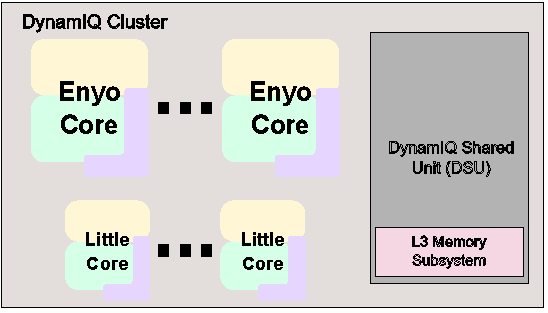
\includegraphics[width=8cm]{img/arm.pdf}
	\bicaption{ARM A76的大小核架构\cite{arm76}}{ARM big.LITTLE architecture of A76}
	\label{ARM的大小核架构}
\end{figure}

虽然延迟可以近似理解为在特定资源上的工作负载,但是在ARM硬件中,CPU存在大小核的情况,即某些处理器有一些性能更高的大核心和一些性能较低的小核心\ref{ARM的大小核架构}。对于一个相同计算负载的任务,在大核心上会具有更小的延迟,移动端推理框架比如ncnn和paddlelite等框架\cite{febvay2020low}就提供了运行时功耗级别的设置,实质上就是通过绑定大核实现高功耗模式,绑定小核实现低功耗模式。最好的情况下,我们还希望能捕获这种更细致,更底层的信息作为优化参考,但基于\ref{现有计算机视觉算法延迟观测的一般方法与不足}所描述的一般日志系统,这类元信息的获取就性能负载而言并不廉价。

总结本节,模块延迟作为一种重要的任务负载评估数据,在计算图调度过程可以发挥相当多的作用。但一个相同功能模块的延迟不是一个确定的常数,而是需要根据具体的部署状态去进行测量,依赖于一个高效灵活的延迟观测系统来辅助完成这一工作。

\subsection{优化参数设置}\label{优化参数设置}
部分参数的设定也会影响系统的性能,一个比较常见的指标是线程池的大小设置。线程池是一种用于管理和调度线程的技术,可以有效地利用系统资源,提高系统的性能和响应速度\ref{线程池的工作过程}。对于计算机视觉任务来说,其关键瓶颈通常在模型推理部分,要尽可能的减少其等待时间。线程池可以预先创建一定数量的线程,每当获得模型的输出,快速为推理模块填充新的输入。视觉算法通常需要处理大量的图像和视频数据,需要大量的并发和并行,因此线程池可以带来良好的重用,减少线程的创建和销毁造成的系统负荷,但也需要根据具体的应用场景来进行评估和调整,例如根据延迟信息代表的工作负载,避免设定太多的线程造成过过度上下文切换,同时也应该考虑内存占用的问题,这一点在嵌入式系统的边缘计算中尤其重要\cite{threadpool}。

\begin{figure}[htbp]
	\centering
	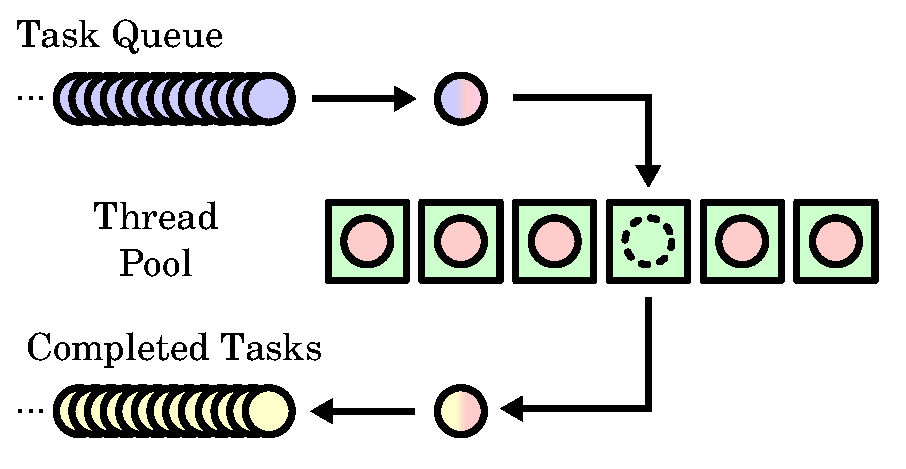
\includegraphics[width=8cm]{img/thread_pool.pdf}
	\bicaption{线程池的工作过程}{The working process of thread pool}
	\label{线程池的工作过程}
\end{figure}

延迟的观测不止存在一个维度,对于\ref{基于计算图的模块抽象}中的推理模块,其运行的延迟可以进行数据分布的统计,考察同一类模块执行计算任务时间开销的变化情况,也可以选择根据以数据本身为观测维度,即数据从进入计算机视觉算法系统开始,到获得对应的结果信息对应在每个环节的延迟开销。这当中必然还存在一些调度时间,例如在线程池中排队等待响应。如果等待时间占比太长,发生的线程调度过于频繁,则说明线程池设置的规模太大,参数配置并不合理。

\subsection{事后追踪参考}\label{事后追踪参考}
日志的事后追踪能力是指在程序运行过程中,将程序的关键信息和状态记录下来,并保存到日志中,以便在程序出现问题或异常时,能够通过分析日志来查找问题和排除故障。计算机视觉算法在运行时的延迟信息和元数据,包括时间戳、线程ID、进程ID、运行环境,以及可以控制颗粒度的,具体在哪一个模块运行这样用来描述程序执行路径的上下文信息。这样的筛查能力可以在端到端的总体延迟出现波动时,可以快速排查到出现故障的模块,提供一种可定位性。

大部分边缘业务因为数据和安全性的考虑,基本只在内网环境运行,本质上相当于离线状态。当出现一些偶发的故障,需要排查和处理,由于嵌入式系统的部署特点,一般只能通过对历史故障的描述,至少在几个小时或者几天后,先将服务下线,然后才能开始尝试复现故障问题,这种重现由于缺少参考信息,一般非常困难。

\begin{figure}[htbp]
	\centering
	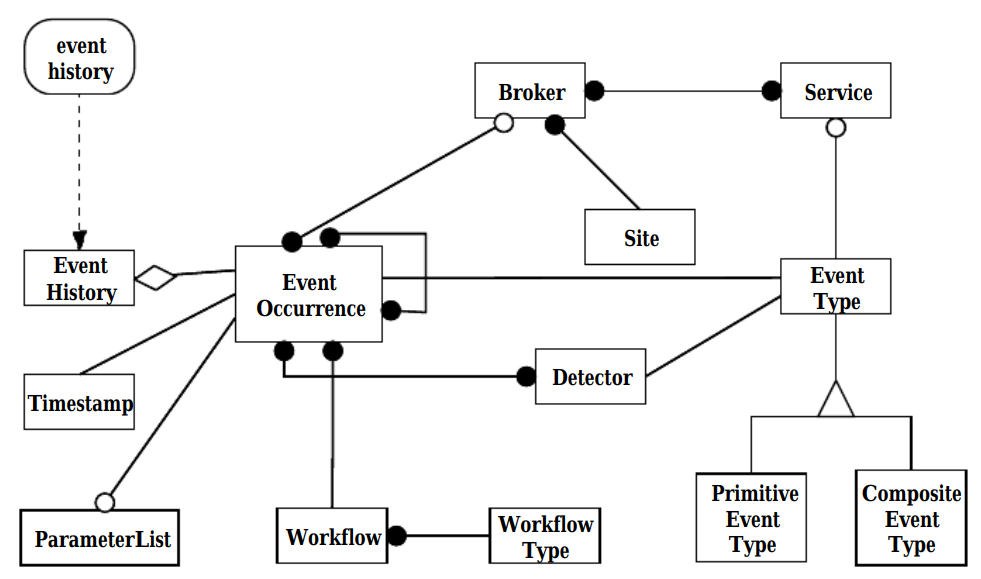
\includegraphics[width=8cm]{img/eve.png}
	\bicaption{一种日志事件跟踪的设计方法\cite{geppert1997logging}}{
		A Design Method for Logging Event Tracing}
	\label{一种日志事件跟踪的设计方法}
\end{figure}

事后追踪能力主要就是为这一情况提供帮助。本文讨论的延迟数据,一个重要作用,就是可以通过延迟数据日志来定位故障发生的时间点,以及根据延迟出现异常波动的具体环节,推测故障发生的位置\cite{geppert1997logging}。特别的,延迟的元信息,即软件硬件的状态信息,由于是一种“活体观测”的运行时数据,因此非常宝贵,相当于不需要重现故障,就可以获得事件发生时的部分图景。

\section{本章总结}\label{本章总结}
本章的主要目的是定义问题,明确需求。延迟作为一个两端时间戳的差值,首先需要明确测量的具体方式。本章首先描述了基于计算图和模块封装,来定义和实现计算机视觉算法部署的一般方法,之后具体描述了基于选择器和采样点的设计方案,阐述了算法延迟的提取过程,并对技术选型进行分析,最后探讨了记录延迟数据在计算机视觉算法部署工程中的作用。

\chapter{轻量级视觉算法部署延迟观测系统实现}\label{轻量级视觉算法部署延迟观测系统实现}

\section{延迟观测事件构造}\label{延迟观测事件构造}
\ref{基于计算图的模块抽象}描述了一个计算机视觉算法在部署过程中,一种工程上的封装方式。即业务流程可以被表达成多个模块的组合,通过对模块的串联实现并行和并发控制,而框架,硬件,实现上的兼容被封装在模块的具体内部实现当中。

\ref{计算机视觉算法延迟的提取方式}描述了基于上述封装,论文所描述的计算机视觉算法延迟的提取方式。其核心思路是将对延迟的观测功能外置,实现为独立的工具。基于设置阶段这一概念,允许通过配置和修改配置文件(Config)的方式,选择具体启动模块上的哪些采样点来工作,实现了业务软件的运行和观测本身解耦。
“热插拔”和“低耦合”的方式,不仅在延迟收集的过程中带来了便利性,避免反复编译程序主体,同时,在边缘计算的嵌入式场景下,“按需采集”的延迟提取有效的限制了实时观测程序对算法吞吐和响应时间的影响。
论文所述方案是一种基于事件(Event)的响应机制,而其良好的性能表现则是依赖于操作系统使能的动态追踪技术。本章节从延迟观测事件的构造开始论述,进而介绍了如何获取完整的延迟信息和硬、软件状态信息,以及最终如何跨越用户态和内核态获得结果。
\subsection{动态追踪技术概述}\label{动态追踪技术概述}
动态追踪技术(Dynamic Tracing)\cite{keniston2007ptrace}是一种后现代的调试技术,其诞生动机就是面对更加复杂的观测场景,提高对于整个生产系统的可观测能见度和控制力,和\ref{使用元数据拓展观测维度}所描述的早期UNIX工具不同,其强调对于开发人员的高度可拓展性,设计理念就是面向运行时调试。

早期的动态观测工具由Sun的DTrace\cite{gregg2011dtrace}推广,被广泛迁移到各种软件平台。DTrace提供了一种语法类似于C脚本语言D,支持以特殊的语法在某个内核函数或者用户态函数的入口或出口,甚至是任意一条程序语句或机器指令上放置一种“探测点”,这种对系统可定制的掌控力得到了众多复杂系统软件开发者的认可,但包括后续的SystemTap\cite{prasad2005locating}等工具,或受限于内核的集成度,导致兼容性和便利性缺乏,或是受限于这种可观测能力实现的工程水平,可编程性和安全性不足。

eBPF(extended Berkeley Packet Filter)是Linux内核中的一种机制,它可以动态地将特定的代码片段加载到内核中,从而实现对系统行为的监控、跟踪和控制。eBPF承接早期动态追踪工具的思路,但充分受益于现代开源生态。基于BTF指令虚拟机在内核运行,利用LLVM编译器保证其生成代码的安全性和效率,实现语言层面的高表达能力和拓展支持,同时和Linux系统紧密集成,作为内核的子模块,不仅保证了效率,也保证了兼容性。目前已经快速成为内核中,最被关注,发展最快的子模块之一,以低开销提取细粒度的观测数据,为性能评估和故障分析提供分析与参考,被称为可观测性的黑魔法。

\begin{figure}[htbp]
	\centering
	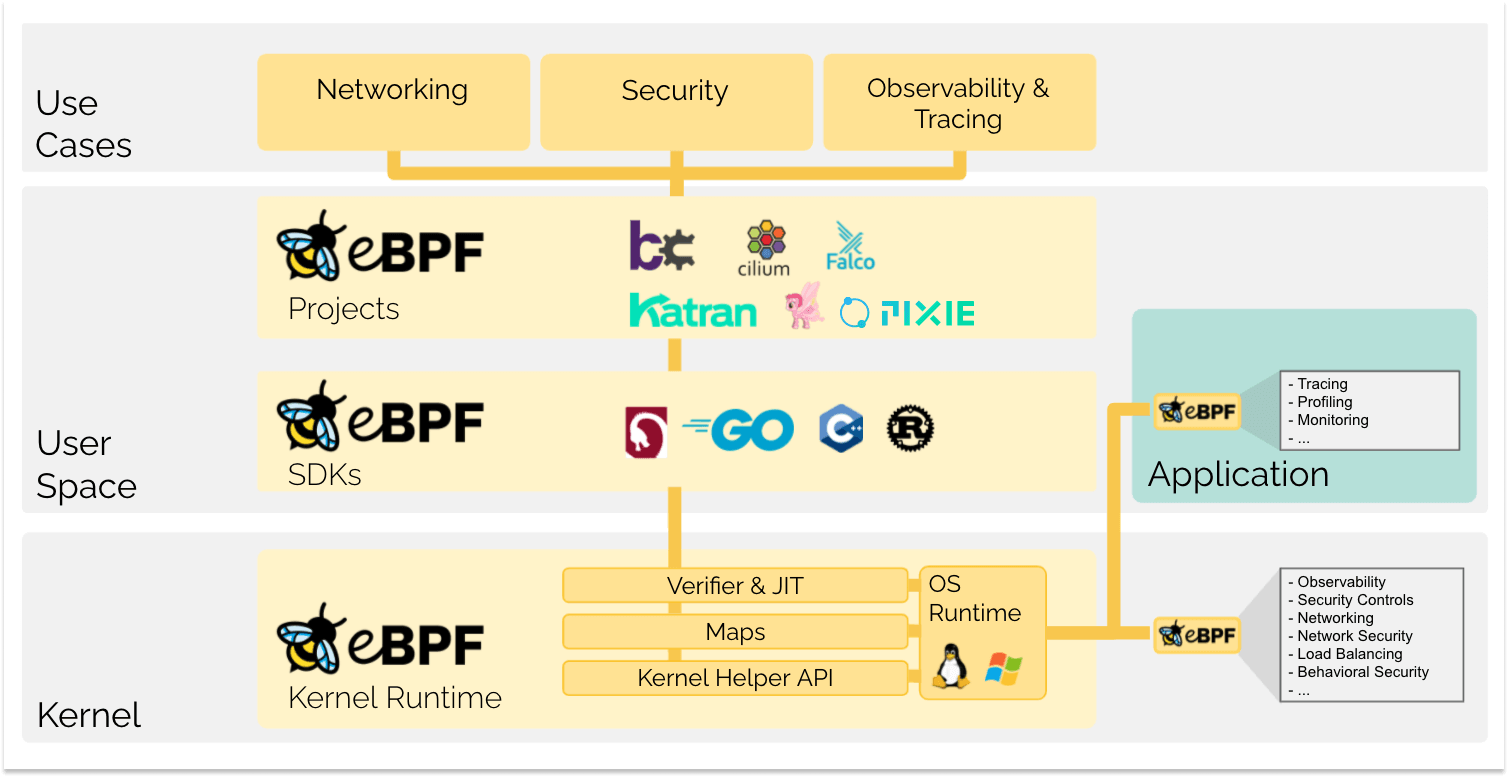
\includegraphics[width=8cm]{img/ebpf.png}
	\bicaption{eBPF概览\cite{whatisbpf}}{eBPF overview}
	\label{ebpf概览}
\end{figure}

BCC是eBPF生态的最早开拓者,因为效率尚可,开发简单,在Meta和Netflix被选择为主力观测工具,社区工具发展齐全,软件接口丰富,但依赖于编译器Clang(类似Systemtap),有运行时编译的性能问题,需要超出工具本身运行开销的硬件条件来进行编译工作,且内核的头文件也需要安装在目标主机,如果使用多个不同版本的内核,会造成调试和兼容的混乱,并且最终的软件包体积也较大,因此适合在普通的服务端的领域使用,而不适合论文所讨论的边缘计算环境。

BPF CO-RE(Compile Once-Run Everywhere)实现了一次编译,处处运行,旨在解决eBPF程序的可移植性问题,该形式可以在任何支持BPF的内核上加载和执行。这为运行程序提供了标准化、可移植的接口,类似于Java字节码在不同平台上运行的方式。目前的新版本的内核和BPF社区,支持了以C/C++接口对的BPF CO-RE的封装,它为用户空间程序提供了和内核中的BPF程序通信,加载、管理的方法,提高了程序的可移植性和可重用性,足以支持进行一些嵌入式环境下的使用和开发,来实现传统观测工具无法获得的性能和功能。

\subsection{基于阶段的延迟选择功能实现}\label{基于阶段的延迟选择功能实现}
在\ref{论文观测机制示意图}提到的基于阶段选择方式,需要实现一些可以捕获信息的“采样点”,这种采样点需要能通过独立的观测系统打开和关闭,且关闭时不会造成额外的性能开销,打开时不影响程序的运行。这一概念类似生物学上的“探针”,能在不用机器下线,甚至不用修改代码的情况下,如何定位和分析取决于另一套机制和原理,只需要在需要观测的时插入用于采样的探针,问题有了针对性的解决方案以后,再把探针移除。

实现这一功能显然需要来自更高级别的权限支持,在软件运行的过程中,操作系统拥有绝对权限和可见度,非常适合承担这一任务。基于eBPF实现这一功能,依赖于一种叫插桩点的机制。根据实现方式和用途的不同,分为静态插桩点和动态插桩点。论文所述场景中,插桩点放置在计算机视觉模块的出入口,属于用户态程序,因此主要使用的插桩点种类为USDT(User Statically-Defined Tracepoint)。

USDT的实现机制基于静态插桩(Tracepoint),在现代内核中,这一机制支撑了\textbf{perf}\cite{de2010new}这样的工具,也是MySQL、Java、PostgreSQL、Node.js等知名项目的运行可观测性实现方法。USDT的开启和关闭,则是通过操作系统加载程序代码的特殊操作实现。当采样点没有启动时,对应的位置是一条\textbf{nop}指令,不起任何作用,当BPF的观测开启,会被替换为\textbf{int3}的(断点汇编指令,breakpoint),陷入内核中断,之后挂载预先编写的BTF程序。这种机制完全基于操作系统来实现,代价只是一种指令跳转。
\begin{figure}[htbp]
	\centering
	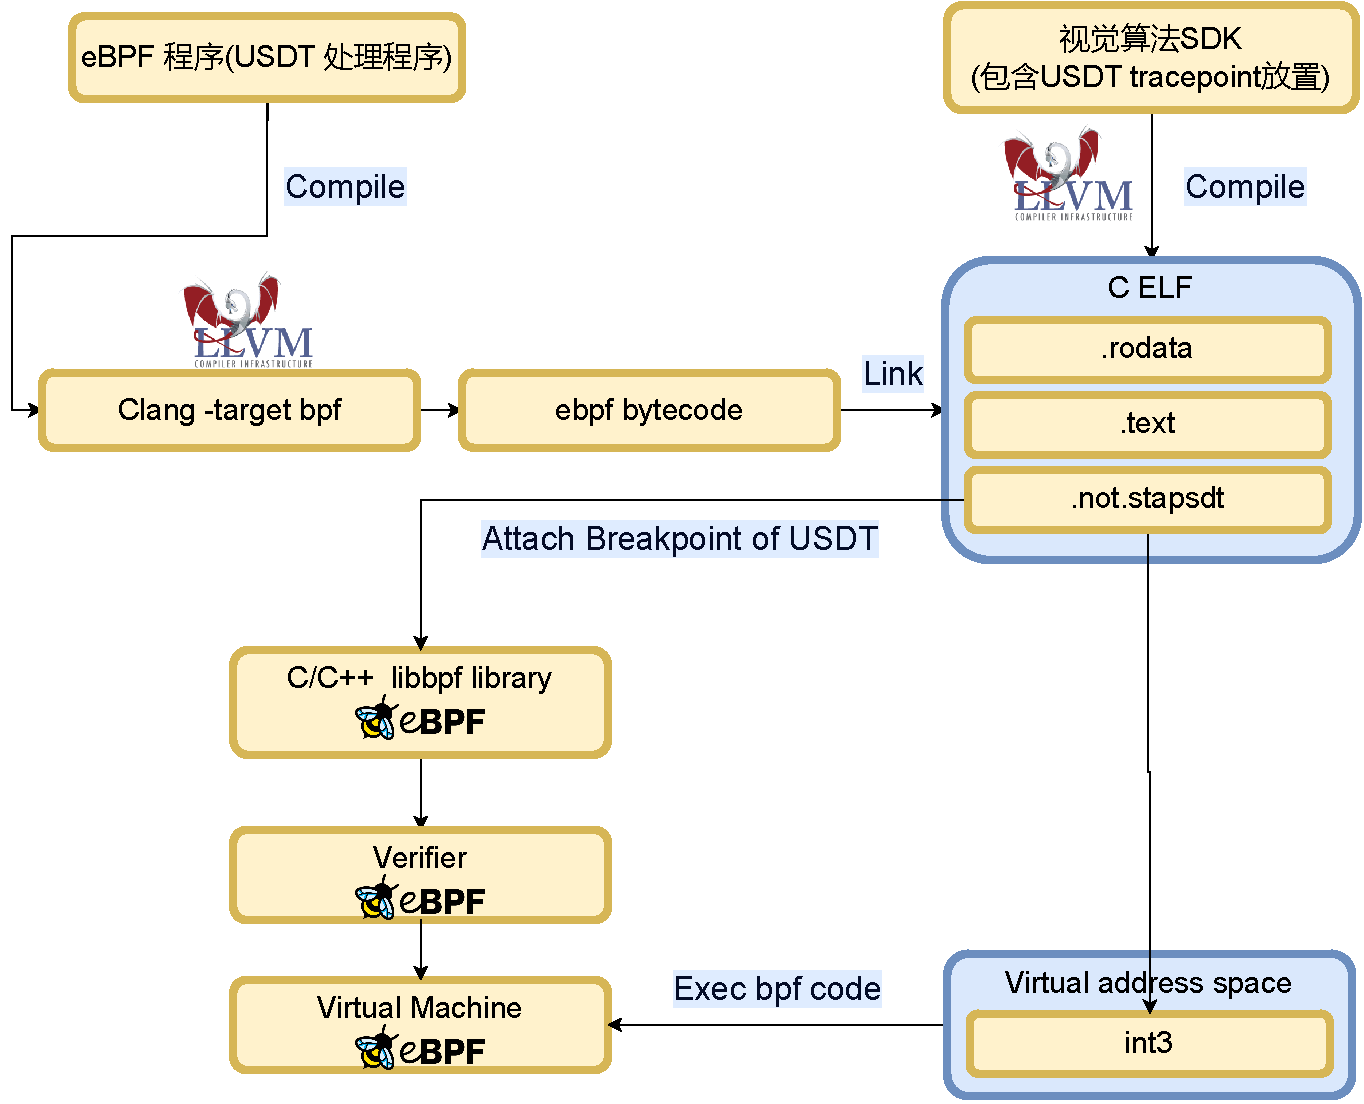
\includegraphics[width=8cm]{img/usdt.pdf}
	\bicaption{USDT构造视觉算法运行时采样点}{Construct computer vision algorithm runtime sampling point by USDT}
	\label{使用USDT构造视觉算法运行时采样点}
\end{figure}

\ref{计算机视觉算法延迟的提取方式}所述的方式是一种阶段选择,但操作系统无法预先了解哪些追踪点需要开启,这些观测点只能全部打开,或者全部关闭。因此,这种“选择”下,跳转的过程一定会执行,只是会根据配置信息,决定后续处理是否继续。实践中无需担心这种仅有跳转的开销,即便采样频率到达每秒数千次,因为代码路径很短,性能开销仍然可以忽略。对于选择这一基础功能,论文所述方案的处理方式是预先编写一个配置文件(Config),描述具体需要处理哪些观测点,这个信息会被提前读取到内存中,在跳转后,采样点的执行代码会优先查看后续流程是否需要执行,如果不需要处理则直接返回。

\begin{figure}[htbp]
	\centering
	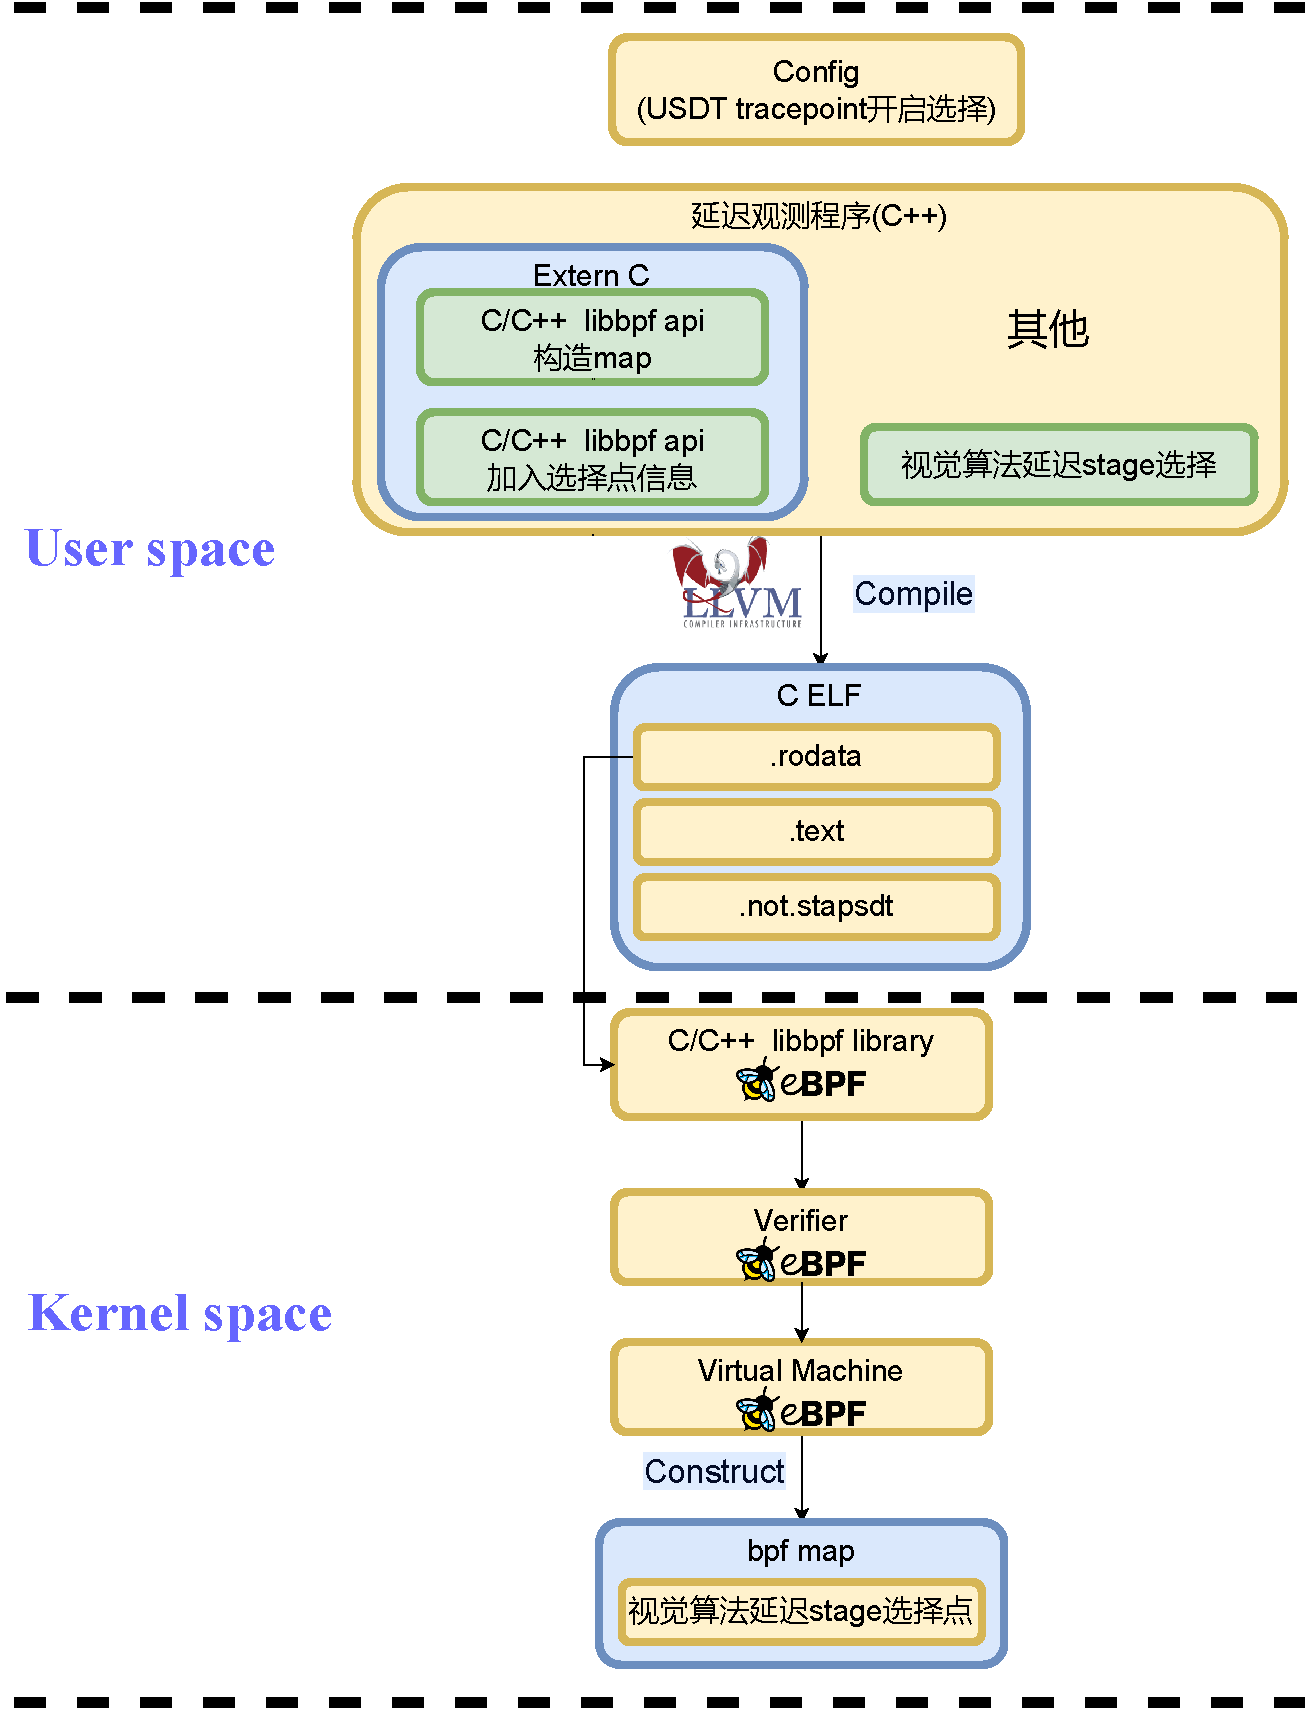
\includegraphics[width=8cm]{img/maps.pdf}
	\bicaption{使用BPF-map实现采样点选择}{Implement sampling point selection by BPF map}
	\label{使用BPF-map实现采样点选择}
\end{figure}
由于这是一个存储键值后进行查询的过程,因此可以使用哈希表来进行实现。这一实现的难点在于,在用户态读取的选择节点的配置信息,创建得到的哈希表无法让内核态的代码进行查询。论文的实现方案依赖于BPF自身支持的一种特殊map,这种map基于BTF的指令实现,会直接在内核态进行构造。使用eBPF时,用户可以创建一个共享的map,并使用其在多个eBPF程序之间共享数据。这个map可以在内核空间创建,也可以在用户空间创建并传递给内核。多个eBPF程序可以同时访问map中的数据,允许它们共享对同一组数据的访问。这种方式可以提高效率,减少数据拷贝和上下文切换的开销,并支持高效的跨进程数据观测。

\begin{lstlisting}[caption={一种在BPF代码中的实现过滤的方法},captionpos=b]
SEC("IO_module_in")
int BPF_USDT(USDT_IO_module_in, void *arg1, int camera_id)
{
	if (camera_id != target_camera){
		return 0;
	}
	//do process
	return 0;
}
\end{lstlisting}

基于这种方式,可以还实现一些特殊的过滤,例如在计算机视觉的场景中,假设模块中增加一个代表输入摄像头编号的参数\verb*|camera_id|,则可以只跟踪指定的摄像头产生的数据。类似的定制化的过滤,一般修改观测装置的代码即可,对普通开发者而言不算困难,实现一些更高级的过滤可能需要从内核读取一些数据,实现方式可以参考stortrace\cite{stortrace}中的实现。


从最终的结果上看,基于阶段的延迟选择功能实现,主要分为两个步骤。第一步是在整个计算机算法部署的各个模块,各个层次,安置上USDT,这之后,构成部署算法运行的计算图各个模块,即便跨越了不同的进程地址空间,不同的异构计算硬件,借助操作系统内核,最终独立的延迟观测系统依然能把不同层次的“探针”收集起来。第二步是实现配置的解析,观测方式配置,挂载预先编写处理程序的“选择器”部分,负责独立延迟观测系统的初始化。


\section{延迟观测事件的信息获取}\label{延迟观测事件的信息获取}
\ref{延迟事件观测}描述了对于NVIDIA平台的GPU,可以通过具体的API去获取硬件状态信息这种相对简单的方式。国内的ASIC计算硬件驱动程序通常功能较少,一般没有稳定的观测API,主要的硬件信息和状态通过debugfs来进行输出。

Debugfs是一个基于内核的文件系统,用于在调试和性能分析过程中提供底层信息,通常安装在\verb*|/sys/kernel/debug|目录下。其不仅可以访问一般硬件例如CPU和内存的使用情况,还可以通过一些定制化的接口,读取设备驱动程序信息。

NPU(Neural Processing Unit,神经处理单元)是一种专门用于进行人工智能和深度学习计算的处理器。与通用处理器相比,NPU具有更高的计算效率和吞吐量。在嵌入式设备中,NPU通常是作为一个独立的硬件模块来实现的,这属于一种定制化的ASIC硬件,此处讨论以后续实验中使用到的RK3588S处理器为例,这款微芯微(RockChip)设计的处理器包含4个ARM Cortex-A76核心和4个Cortex-A55核心,板载一个6Tops算里的INT8专用NPU,实验所用的这款主板与2023年开始陆续销售,是目前最具代表性的国产ASIC芯片之一。

参考芯片官方提供的固件文档,其CPU和NPU等,甚至包括DDR和电源等硬件的各个硬件单元的频率都是动态调整的,目前仅支持通过debugfs的方式进行查看,结合常规的优化需求,以CPU和NPU为例
\begin{lstlisting}[caption={命令行查看rk3588硬件参数信息},captionpos=b]
// 查看CPU频率
cat /sys/kernel/debug/clk/clk_summary | grep arm 
// 查看NPU的利用率
cat /sys/kernel/debug/rknpu/load 
// 查看NPU的当前频率
cat /sys/kernel/debug/rknpu/freq 
\end{lstlisting}


\begin{figure}[htbp]
	\centering
	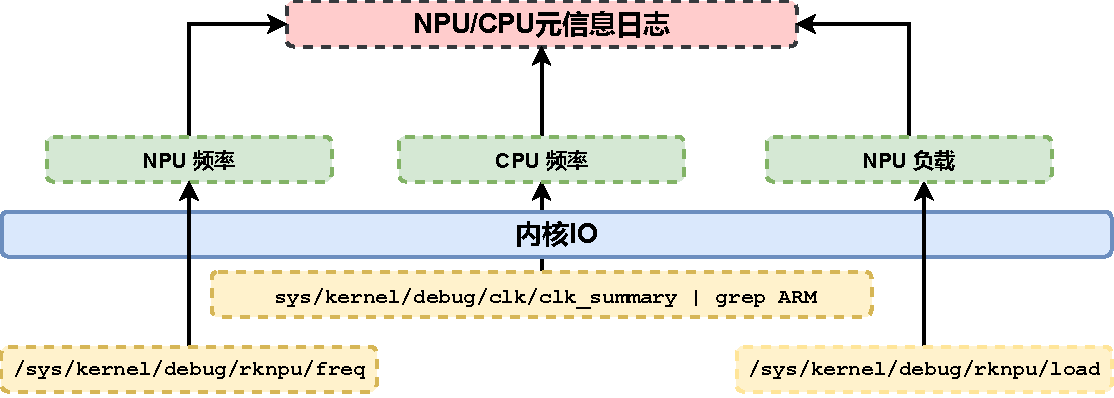
\includegraphics[width=12cm]{img/readk.pdf}
	\bicaption{读取上述硬件信息需要的内核IO}{Kernel IO required to read the above hardware information}
	\label{读取上述硬件信息需要的内核IO}
\end{figure}
参考\ref{读取上述硬件信息需要的内核IO}图示,如果采用官方提供的API,至少需要从debugfs进行三次内核IO读取,才能对日志中关于CPU和NPU的元信息部分进行采样。如果还需要额外的信息,例如必须获得的时间戳,一些程序上下文等,则每一次对内核信息的采集,都需要反复的进行内核态到用户态的上下文切换,造成显著的性能开销。



总结两种不同硬件,虽然获取状态信息的底层实现方式各有不同,但都存在当需要获取多个状态信息时,只能逐次在用户态进行系统调用的问题。

由于在采样点的跳转后,程序已经进入了内核态,因此利用\verb*|libbpf|的API,在内核态一次性获取全部数据,可以改善这一点缺陷。当运行于用户态的程序,在触发延迟观测事件,BPF程序允许在编译器的安全保证下,编写一些受限制的,对内核的只读,不具有破坏性的代码,这种对内核的可编程性极大的拓展了我们获取底层信息的方式,例如上文中NPU存放于debugfs中,正常的读写方式只能通过标准文件IO,再进行文本处理。而\verb*|libbpf|编写一些BPF程序的过程中,可以直接使用一些内核头文件的非系统调用(\verb*|#include<linux/debugfs.h>|),这一方式在未来甚至可能在非root权限下执行,具有更好的生产安全性。

\begin{lstlisting}[caption={使用非系统调用方式读取debugfs},captionpos=b]
unsigned long bpf_probe_read(void *dst, \
	u32 size, const void *src);
struct file *file = debugfs_open("my_debug_file", O_RDONLY, 0);
bpf_probe_read(&my_debug_data, \
	sizeof(my_debug_data), file->private_data);
fput(file);
\end{lstlisting}

GPU还有一些特殊的观测方法,例如直接利用\verb*|bpf_core_read|来读取利用cudaMallocHost固定(pinned)在的内存,这种做法一般使用在对性能苛刻,且官方没有支持的情况。

由于计算机视觉算法部署的延迟观测中,查看延迟本身至少就需要一次系统调用的开销,通常还需要获取其他底层元数据,无论是硬件状态还是软件状态,基本都无法在用户态获得。通过\verb*|libbpf|的实现方式,对时间戳的获取被\verb*|bpf_ktime_get_ns|替代,而其余根据具体的信息位置不同,也可以一次性获取,无需再切换到用户态,只有一次系统调用的上下文切换开销。上文和\ref{延迟事件观测}是两种获取硬件状态典型方式,而操作系统的软件上下文相对更加简单,原则上优先使用\verb*|libbpf|支持的API,不支持的再通过直接读取内核地址实现,基于LLVM检查,无需担心对内核造成不安全的隐患,风险代码会直接编译失败。


\section{基于元数据的观测维度拓展}\label{基于元数据的观测维度拓展}
以上描述了基于内核的静态追踪点放置,通过外置传入配置信息,实现了采样点开启和关闭的实现过程。以及如何利用\verb*|libbpf|的可编程性,在一次进入内核态之后,尽可能的完整获取需要的数据,减少上下文切换的开销的一种实现思路。此时考虑实现在\ref{使用元数据拓展观测维度}使用元数据拓展观测维度的问题,通过一些软件上下文的元数据,将来自不同采样点之间的信息进行整合,构建阶段整体的延迟观测信息,来实现对于整个数据运行的链路进行观测。

\begin{figure}[htbp]
	\centering
	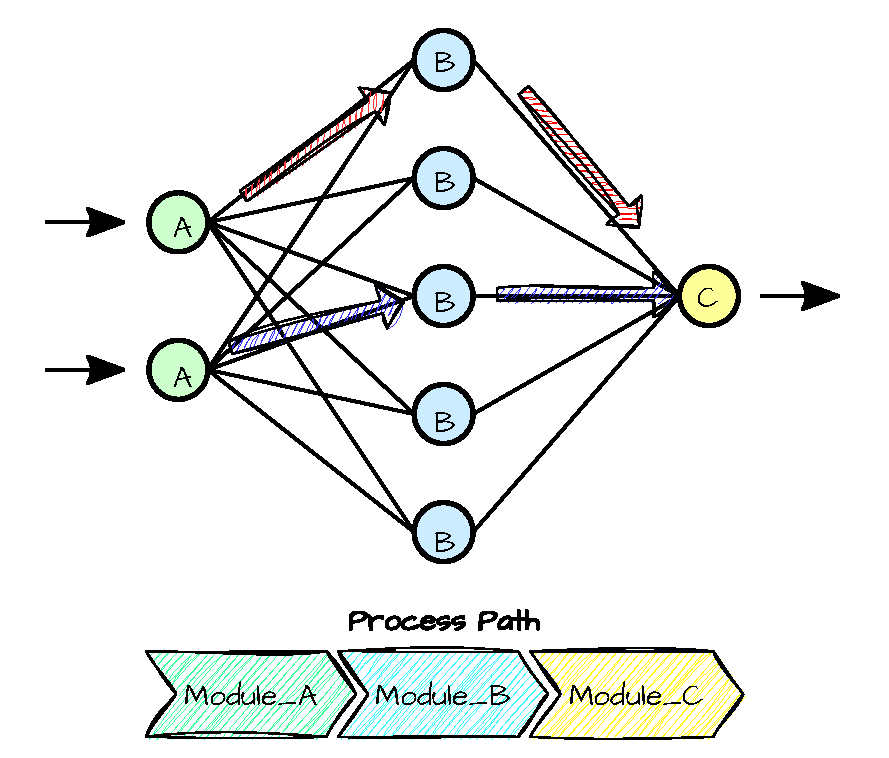
\includegraphics[width=8cm]{img/path.pdf}
	\bicaption{红蓝不同路径在计算图中通过相同的模块}{Red/Blue pass through the same modules in the computation graph}
	\label{rbpath}
\end{figure}


基于计算图的部署算法表达中,对于任何一个执行的路径而言,数据所经过的处理模块种类和顺序一定相同。例如Two-stage的目标检测算法\cite{burke2017meta},最后需要经过非极大值抑制(NMS),用于目标检测中提取分数最高的窗口, 假设此时进行NMS算法处理的实例化模块有2个,来保证GPU(ASIC)保持高吞吐率,此时虽然数据会通过两个不同的模块,但对应同一环节,其需要从采样点中获取的数据是一致的。这一特点可以归纳为,计算机视觉算法和一般的服务运行相比,并不需要通过堆栈去回溯调用路径,因为对于某一种设计好的阶段,其经过的模块是固定的,需要收集的信息也是固定的。如\ref{rbpath}所示,红蓝箭头代表数据的在计算图中的传递,\textbf{A},\textbf{B},\textbf{C}代表三种不同的节点,但即便数据经过的路径不同,执行的模块处理依然一致。

如果想要实现对表示阶段信息的数据结构体进行动态生成,对于C++这样不支持RTTI(Run-Time Type Identification)的语言来说非常困难,因此目前这一部分主要还是依赖于手工编写,需要具体对数据的路径去编写一个方便序列化和分配空间的结构体(Struct),在进入路径开始时就完成内存分配,构造一个对应阶段的日志条目(Log Entry),当经过开启的节点时,则填充对应的数据。

此时的问题在于如何在不同的模块环节衔接,定位到匹配的日志条目,最终归档到同一个阶段。这一过程同样可以利用\ref{使用BPF-map实现采样点选择}中所描述的bpf内置的高性能哈希表,将整个查找和赋值全部放在内核态来执行。

本文中所属的场景有两种可行的方法,一种是在所以的模块参数信息中,加入一个可以作为主键(Primary Key)的参数,每次陷入内核态后(int3),直接从\verb*|struct| \verb*|pt_regs| \verb*|*ctx|(Registers and BPF Context)寄存器上下文中获取到这个主键, 然后从存储对应阶段map中查找匹配的日志条目指针,通过指针进行赋值,当运行到阶段最后一个模块,一次性提交整个日志条目到用户态,并在内核态中删除。这种主键的构造可以通过UUID(Universal Unique Identifier)等方式,适合需要掺杂一些特殊内容和规则的场景,例如\verb*|UUID_设备编号|的形式就可以用于设备日志分流\ref{基于阶段的延迟选择功能实现}。另一种是仅需要构造联系,而不需要再利用这个主键的场景。由于追踪一般以单帧图像作为数据传输,数据本身的地址完全可以作为一个64位整数的主键,因为下一次使用这个内存片段必然已经是处理结束之后的复用,这样的方法可以减少参数传递量。两种方式在stortrace中也均有样例可以参考。

借助内核中的元数据和BPF map,上述方法实现了将从不同进程的用户态程序,操作系统内核,硬件驱动采集到的信息,基于一些维度,例如时间,把任务和数据流转的的完整图景关联起来,从而指导后续更复杂的分析。

\section{延迟观测信息的日志生成}\label{延迟观测信息的日志生成}
至此,我们已经讨论了所有延迟及其元数据,如何借助BPF技术,在内核中进行捕获和关联,并构造为完整的日志条目。但此时信息尚存在于操作系统的内核态,需要在用户态生成具体的日志,才能进一步处理。
\subsection{延迟观测信息的用户态提交}
BPF中都是栈内存的分配方式,而不像用户态一样去分配堆上的动态内存,其原因是保证安全性。\ref{延迟观测事件构造}提到了论文所述的延迟观测系统是基于事件的,有两层含义,即采集事件仅服务于填充日志条目,而最终日志条目的提交是观测阶段最后一个采样点结束后,将整个日志条目提交到用户态。
\begin{lstlisting}[caption={日志条目保存map},captionpos=b]
struct {
	__uint(type, BPF_MAP_TYPE_HASH);
	__uint(max_entries, 1024*8);
	__type(key, u64);
	__type(value,struct log_entry);
} event_cache SEC(".maps");
\end{lstlisting}

更早版本的BPF中,完成这一提交是基于每一个CPU单独构造一个缓冲区,所有需要发送到用户态的信息,都会利用这个数据结构来进行交互。缺陷在于内存使用效率低下,并需要自己处理事件顺序。Linux内核从5.8开始提供BPF环形缓冲区(Ring Buffer)\cite{bpfring}机制,它是一个多生产者单消费者(Multi Producer Single Consumer,MPSC)队列,可以同时在多个CPU之间安全地共享,通过\verb*|reserve/commit|进行数据发射。

\ref{使用USDT构造视觉算法运行时采样点}所描述的过程已经完成了延迟日志条目的构造,最终通过内核信号(In-kernel Signal),即\verb*|poll/epoll|来通知用户态程序来处理。这一过程使用了一种基于Memory Mapping的环形队列,这一数据结构目前广泛用于现代Linux内核。整个日志提交的过程如图\ref{延迟日志向用户态提交的实现}所示,首先需要将内核中的日志条目拷贝到用户态,BPF的Ringbuffer避免了这一开销,其原理是利用了\verb*|bpf_ringbuf_reserve|,内存直接在环形队列上分配,提交到用户态之后,基于Memory Mapping直接可读,避免了额外的内存复制。用户态只需要获得日志条目的构造信息,就可以用\verb*|reinterpret_cast|的方式,重新将环形缓冲区上的数据序列化,进行之后的处理。

\begin{figure}[htbp]
	\centering
	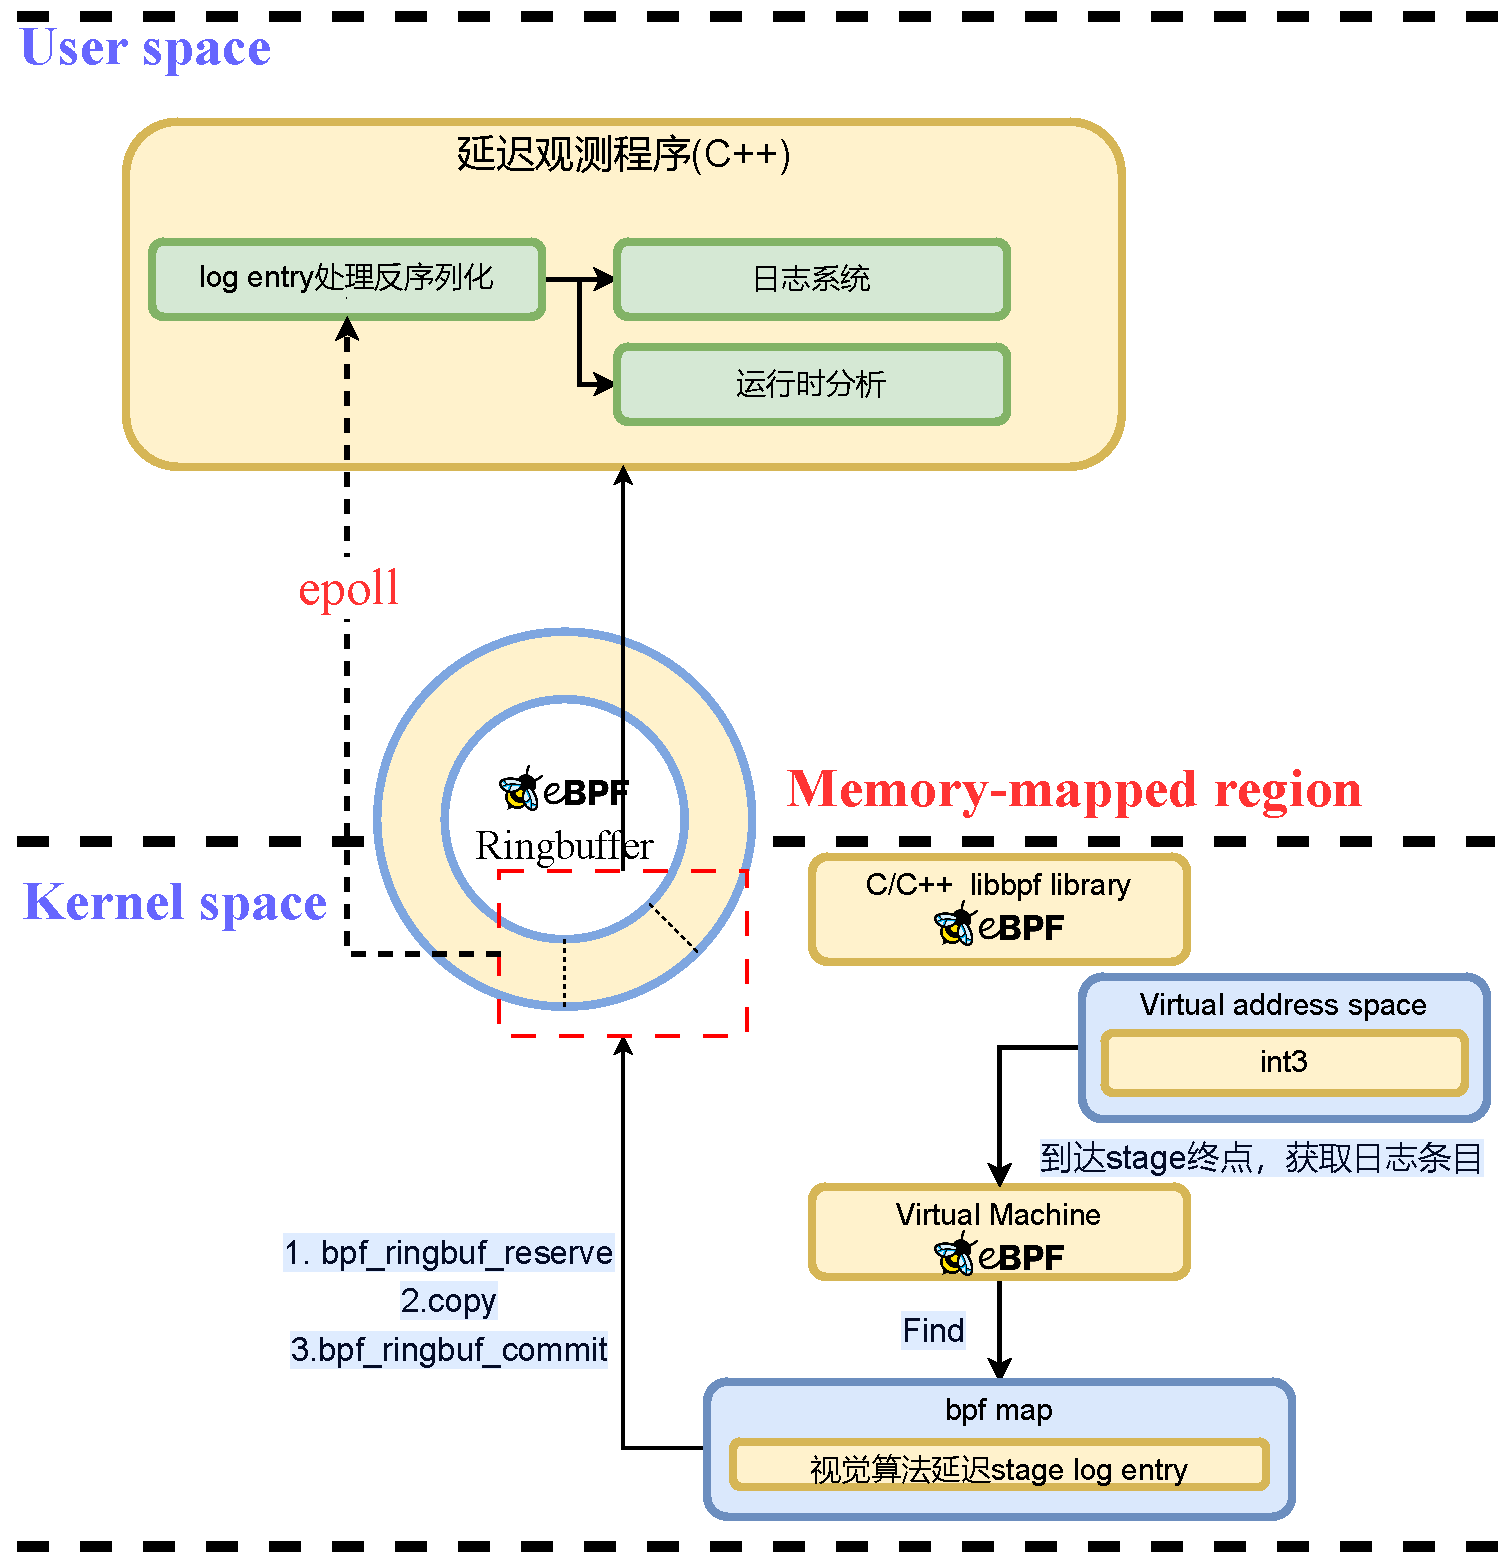
\includegraphics[width=10cm]{img/log.pdf}
	\bicaption{延迟日志向用户态提交的实现}{Implementation of latency observation log entry submit to user space}
	\label{延迟日志向用户态提交的实现}
\end{figure}


\subsection{针对延迟信息特点的二进制格式生成}

回顾\ref{延迟事件观测}中,基于代码注入的日志记录来保存数据,需要先从内存中的变量,生成文本字符串,这种方法既可以简单被初学者实现为打印语句来辅助Debug,也可以实现为GLOG\cite{toubiana2011analysis}这样被广泛采用,效率和功能都被深度优化的日志库。在更复杂的大型分布式系统中,记录会以RPC的形式提交给单独的日志进程,集中的写入和处理。

通过字符串直接打印的数据,一个缺陷是不利于解构使用。因此在现代的通用日志系统中,更多的会使用结构化的格式来对收集的信息进行描述。例如JSON,信息被组织为键值对的形式,每个键代表一个属性,每个值代表对应属性的值,当需要描述更复杂的结构,Bugzilla\cite{serrano2005bugzilla}甚至专门创造了一种专用的标记语言格式(类似HTML),这种格式称为“Bugzilla markup”或“Bzr”。Bugzilla用Bzr格式来记录许多不同类型的事件和注释,包括对Bug描述的更改、新的注释、附加的补丁等等,其也支持使用JSON来进行转换和读取。

这一日志信息的生成方式,主要优点在于良好的格式,便于传输和处理,使用标记和键值的描述,非常利于阅读和理解,也具有很强的拓展性,可以灵活增加新的条目。同时,结构化格式还有利于日志在网络传输过程中的序列化(Serialization)和反序列化(Deserialization),更适合应用在类似前文\ref{基于发布订阅的边缘计算日志系统}提到的具有一定规模的发布-订阅边缘计算日志系统。

但考虑到嵌入式场景下,硬件资源受限,相比兼容和易用,应当优先考虑性能开销。在对具有一定结构的数据对象进行序列化的过程中,需要将数据结构中的各种元素进行逐个解析和编码,将其转换为目标格式所要求的形式,这个过程通常需要消耗一定的CPU时间和内存空间;反序列化过程中,需要对序列化格式进行逆向解析和还原,将数据结构中的各个元素重新组合并还原为原始的内存对象,这一镜像的过程同样是使用这类结构化描述的性能负担。尤其是在以模块为单位封装的情况下,当模块依赖于RPC进行网络模块通讯时,这一开销会因为传输次数的增加而放大,进而对性能和响应速度产生负面影响。

对于以模块为封装单位所构成的计算图,一个数据进入之后各个环节所需要经历的路径可能因为调度的原因有所差异,但其经过的计算模块种类和顺序则一定是固定的,只要处理的流程是确定的,则需要记录的延迟格式也是固定的,分别包含对应模块的时间戳和该类型模块的元信息,差异化只在于延迟数据的波动,即调度执行所导致的偏差值。因此,对于计算机视觉任务这类对具体任务,流程稳定的静态图结构,我们无需JSON这类数据结构格式的长度可变特性,可以生成根据日志条目的格式,生成固定长度的二进制,以确定性的描述方式来换取更低的性能开销。

在内存维护和落盘存储阶段,二进制格式的存储开销要比可读的字符串格式小得多,格式根据采样点的配置组合构成,数据元素之间不需要使用任何分隔符,可以减少不必要的空间占用和数据体积。相比之下,可读的字符串格式通常需要使用分隔符和占位符来区分不同的数据元素和数据类型,并且需要使用更多的字符和空间来描述数据元素和数据类型。使用这种方式不要存储额外的描述信息,即解析的方式以观测点+选择配置文件约定,这类似与键值对的存储中仅保存值信息,这也起到了节约内存的作用。

此外,二进制格式的数据还可以更快地进行读取和写入操作,因为它们可以直接被存储在计算机的内存中,无需进行编码和解码。相比之下,可读的字符串格式需要进行字符串解析和格式化操作,这些操作需要占用更多的计算资源和时间,即便是类似与fmt这类采用现代C++的技术,使用模板元编程和格式字符串解析器的实现,也无法节约运行时的开销,仅能较好的处理好编译期即可确定的日志内容。

实现固定长度的日志信息便于进一步的优化,由于延迟信息产生的频率相对较高,如果每个日志条目都单独写入磁盘,那么需要执行大量的I/O操作,这会增加磁盘访问时间和系统开销,因此对日志信息进行缓存及合并,然后批次写入,是一个有效和直接的有优化手段。但在嵌入式系统中,内存通常是非常有限的资源,如果单个日志条目的大小不固定,且空间占据较大,这种缓存可能会导致内存不足的问题,从而影响系统的稳定性和可靠性。

采用固定长度的二进制日志,不仅提高了存储空间的利用率,并且可以直接计算出缓存一定数量条目所需的空间开销,设置上限,使得日志信息缓存这一措施对于系统的整体影响可控。同时,在复制内存到指定缓存的过程中,如果日志的长度并不确定,由于计算图结构的日志由多个线程生成,则日志的缓冲区可能会被并发的修改,需要谨慎的处理其冲突关系,相对而言,定长日志的缓存区填充和分配实现就非常简单。除去存储以外,在解析的环节,由于日志条目一致,二进制长度相同,因此近似于数据库中的列存储格式,可以实现高度并行化的处理和解析,而不定长度的日志则需要先根据分割符号切割,再进行逐条数据处理。

综合而言,通过设计特殊的二进制格式,总体起到了压缩内存占用,减少落盘IO,以及运行时计算开销等性能提升,代价则是日志信息无法显式的阅读,牺牲了一部分软件层面的兼容性。

\section{延迟日志信息写入}
\subsection{基于IO-URING的异步写入}

日志文件的写入操作是一个相对耗时的系统调用,如果使用同步IO(如标准的文件写入函数),那么当前线程会一直阻塞,直到操作完成为止,这会严重影响程序的响应时间和吞吐量。相比之下,异步IO能够减少线程的阻塞时间,从而提高程序的性能和响应速度。使用异步IO时,写入操作可以在后台进行,不会阻塞当前线程的执行,线程可以继续处理其他任务,不需要等待IO操作完成后再进行下一步操作,这对于高并发的计算机视觉算法执行场景有较好的适用性。

传统C++的异步IO依赖于Boost.Asio\cite{anggoro2015boost}提供的第三方库,其对于早期开发的程序具有更好的兼容性,广泛使用在网络和文件的IO应用,但边缘计算的原生环境一般不会配置boost库,如无必要,应该尽量减少引入额外的软件依赖。

\begin{figure}[htbp]
	\centering
	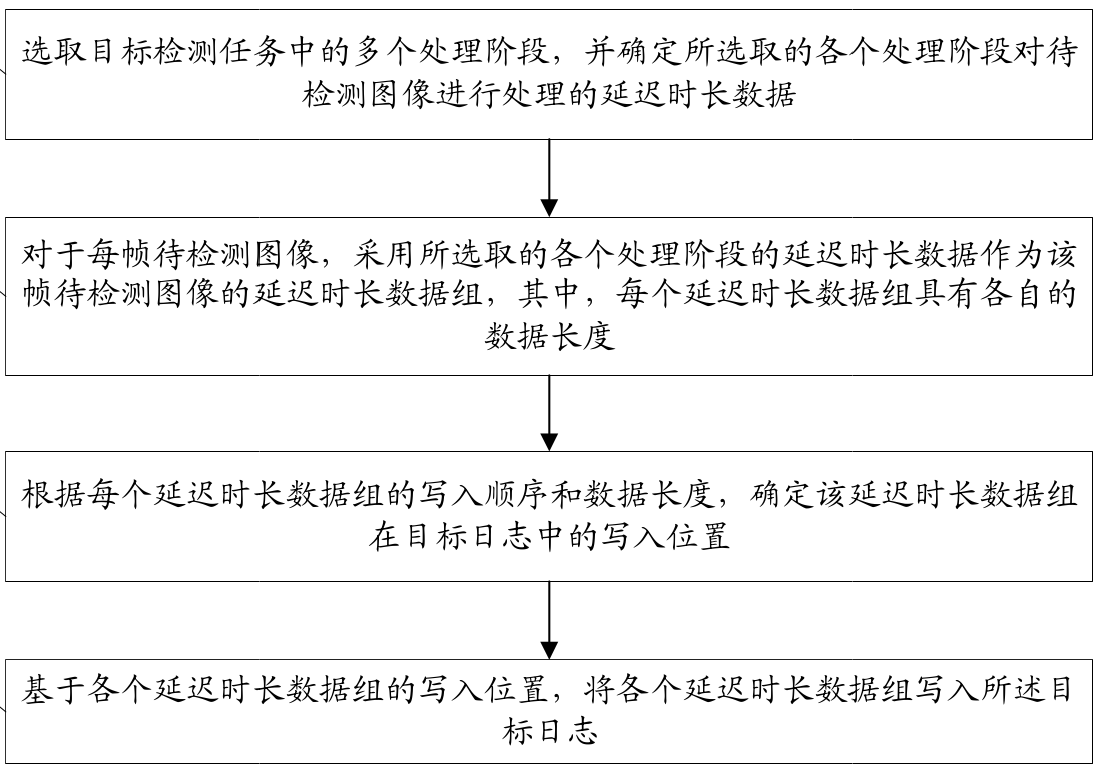
\includegraphics[width=8cm]{img/z1.png}
	\bicaption{延迟异步IO写入方式}{Lantency async write process}
	\label{延迟异步IO写入方式}
\end{figure}

相比之下,由于计算机视觉系统几乎一定是部署在Linux系统中,原生内核异步IO接口\verb*|io_uring|是一个更好的选择。从性能方面来看,Linux的\verb*|io_uring|相较于Boost.Asio更为高效,具有更快的提交速度,以及内核零拷贝数据写入的优势。同时,得益于内核原生的支持,\verb*|io_uring|提供了批量提交IO操作的能力,可以将多个IO请求合并到一个或多个批次中,并将它们一起提交到内核进行处理,这一特性非常适合日志信息这种连续写入的场景,通过批次处理减少写入开销。使用新的内核特性来支持轻量化的日志系统,较好的满足了嵌入式系统开发应该减少依赖的原则。

多个业务共同组合构成的计算图中,为了便于后续的解析和分析,每一个处理路径的日志会被单独归并到一个文件中。
\begin{figure}[htbp]
	\centering
	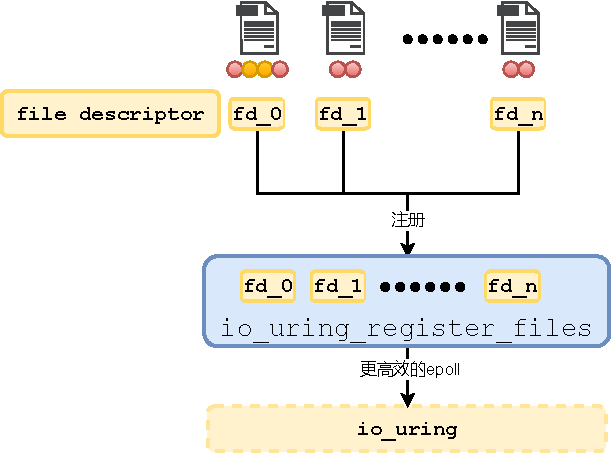
\includegraphics[width=8cm]{img/reg.pdf}
	\bicaption{延迟日志写入优化}{Latency observation log write optimization}
	\label{延迟日志写入优化}
\end{figure}
由于一次观测中,必然存在多个阶段选择,因此需要同时对多个文件进行操作进行追加写入。大部分编程语言屏蔽了异步IO的实现细节,而论文的日志系统实现直接使用内核接口,相比于一般的日志,选择打印到标准IO,或者定向到指定文件中,选择利用\verb*|io_uring|的细节特性来进行优化。在实践过程中,利用了\verb*|io_uring_register_files|接口提前注册文件描述符\ref{延迟日志写入优化},减少IO操作中需要反复打开/关闭文件描述符的开销。这种方式通过预先准备好文件描述符的内核数据结构,在注册时将其加入一个内部的数组,后续IO操作中可以直接使用该数组中的文件描述符,避免了重复查找的开销,降低了系统负载。

我们基于以上设计,实现了一个独立的日志写入程序。这种设计使得写入过程和本身的计算机视觉算法的部署应用相互独立,降低了日志写入对任务进程的影响,有助于保证系统的稳定性。同时,在不依赖第三方库的情况下,深入优化了写入性能。

\subsection{延迟日志的前置过滤}
\ref{延迟观测信息的日志生成}所描述的优化方法,主要是根据延迟信息和计算方式的特点,减少生成日志和记录日志的开销。一般的日志系统中,还有一种更直接的方式是直接减少日志写入的次数,常见做法是通过设置日志的级别过滤,只输出必要的信息。例如GLOG中将日志设置为DEBUG、INFO、WARNING、ERROR 和 FATAL等多个层次,当需要减少日志输出的IO开销,则将日志等级调高,过滤不重要的日志事件。

本文所讨论的是专用于延迟信息记录的场景,所有的延迟都基于数据进出一个计算模块的事件来触发,因此重要性可以视为等价,通过日志等级来进行划分这一方式,不适用于本文所讨论的应用场景。

进而考虑利用延迟信息本身的特点,即由于计算图中的各个模块,可以近似的理解为无状态的函数计算流程,因此一般情况下,基于合理的调度策略,如果不出现故障,一个模块的延迟基本会处于一个稳定的范围,反之则可视为对应节点功能出现异常。在计算机视觉算法的部署过程中,通过观测这些偏移正常波动范围的延迟值,定位出现异常的环节,从而提供优化参考和事后追踪依据,正是记录延迟信息的主要目的之一。

对于同样以模块的形式封装,作为任务纳入计算图范围的,涉及网络传输,磁盘IO操作的模块,其延迟也有类似的特性,即整体表现为长尾分布的特点\cite{dean2013tail},其值在大部分概率分布对应的范围都很小,但在尾部区域,存在一小部分极端值,对整个分布产生重要影响。在网络传输和I/O操作中,这些极端值通常是由网络拥塞和故障等因素导致的,例如网络中出现了大量数据包丢失或重传、磁盘IO调度中发生了不可预测的错误等。长尾分布的特点意味,大部分的延迟信息并无意义,需要更多地关注极端值。

简单总结视觉算法计算模块中的延迟数据特点,一般的稳定延迟信息其实并无记录的必要,重点需要记录的,是延迟出现快速增长的阶段,然后分析对应时间段内的延迟日志信息。由于二进制定长数据格式的延迟信息不需要额外的解析,便于在运行时进行简单的计算,通过设置一个前置的过滤算法,可以在CPU资源能够接受的范围内,通过轻量的运行时分析,判断一条延迟信息是否需要被记录,当判定为正常时,则直接在内存中释放,以此减少日志写入的次数,降低IO系统调用的额外开销。

\subsubsection{延迟前置过滤的判定方法}\label{延迟前置过滤的判定方法}
判定延迟出现快速增长,最直接的方式是时间序列分析中的变点分析(Change Point Analysis)。其主要目的是发现数值随时间波动的过程中,体现出显著特征变化的点位,但这类基于时序模型的方法,需要根据统计来构造概率时序模型,类似于ARIMA\cite{kalpakis2001distance}、Holt-Winters\cite{chatfield1988holt}等,无法做到运行时分析,起到前置过滤的效果。

另一种则是基于回归的方式,织云Metis\cite{xia2019anomaly}是腾讯开源的一个面向微服务的服务质量监控平台,其引入了机器学习算法作为回归模型,基于统计判决和机器学习算法,对时序数据进行联合检测,并构建一个异常检测模型。在运行时,将新的延迟数据输入到模型中,根据模型输出的异常概率判断是否存在异常。因为Metis开源项目侧重于学件的实现,其主要使用Python语言来完成,在性能不可接受,同时,这套基于机器学习+统计判断的方式,在嵌入式系统上运行的代价过于高昂,并且由于部署环境和传统的服务端不同,难以收集到适合训练使用的标注数据集,因此也不适合使用在边缘计算的场景。

代价最小的异常判别方式则是基于阈值,根据不同的业务需求选择合适的阈值来进行判断。一种常见的方法是使用“百分位点”(Percentile)来衡量延时的分布情况。百分位点是指在一组数据中,某个百分比的数据点的值在这个百分比的数据点中是最小的。例如,95$\%$百分位点是指在一组数据中,有95$\%$的数据值比这个百分位点的值小。

在计算机视觉的部署场景下,对于不同模块延迟的稳定性要求不同,可以设定不同的分位数进行异常判别。例如对于部署在5G网络环境下的传输模块,其会受到运营商的调节干预,使用人数和网络拥塞状况也存在一定的波动,可以将目标响应时间设置为95$\%$或99$\%$(P95/P99)的百分位点,以确保即使出现延迟较长的操作,仍然被接受为合理的范围。而对于例如NPU和GPU上运行的推理模块延迟,作为系统核心的吞吐模块,我们希望保持积极稳定的响应频率,则可以将目标响应时间设置为50$\%$,75$\%$左右的百分位点,对偏小的延迟增长也会提出异常判别,将信息记录下来。

这一灵活性更满足了嵌入式系统这类边缘计算的需求。作为一个延迟信息的前置过滤装置,这种实现具有以下几个特点:

\paragraph{灵活性}
相对于使用固定的阈值来判断延迟是否异常,百分位数反映的是延迟分布中的具体位置,可以根据具体模块的响应特点来进行设置,更加适合计算机视觉算法这种需要在异构系统和复杂外环境下部署的场景。

\paragraph{自适应}
嵌入式和边缘计算的环境中,如果使用机器学习算法来对不同软件硬件条件下形成的延迟分布数据进行甄别\cite{zhang2016treadmill},需要重新进行数据集的标注构建和模型的训练,这一点和织云Metis所面对的单一普通云服务部署场景不同。而使用百分位数的方式,数据从实际运行的统计结果中构建,具有对实际分布自行适应的特点。

\paragraph{低性能开销}
基于机器学习的算法其运算代价远高于分位数(Quantile)取值过程,即便判定更加准确,但在嵌入式的环境中仍然不可接受。并且,其通常需要一些独立开发的,针对体系结构深入优化的第三方科学计算库(MLK)来辅助计算,这也会增加开发的难度,降低软件的兼容性,还会引入额外的软件依赖。

\paragraph{可解释性更强}
不同于一些场景下,机器学习做出一些复杂的决策过程,延迟信息本来就是一种偏向于系统运行底层的数据。在计算机视觉算法的部署场景中,设计这一延迟日志信息前置过滤模块的主要目的,是为了减少日志的写入次数降低额外开销,最终对于软件优化的参考和故障问题的追溯依然需要使用人员具体阅读日志结果。因此,百分位数这一更具有可解释性的指标,可能会更满足嵌入式系统下复杂的调试需求。

\subsubsection{基于T-digest的延迟过滤}\label{基于T-digest的延迟过滤}
基于百分位数的异常延迟判断方法,即便计算复杂度低于机器学习算法,但依然需要统计一段时间内的所有延迟数据,并进行排序和计算,仍然还是需要不低的计算资源和内存空间。最终的工程实现过程中,选择了近似的估算方式。

T-digest\cite{dunning2019computing}算法是一种简单、快速、精确度高、可并行化的近似百分位算法,其通过缓存和合并(Buffer-and-Merge)的方式来动态刻画一个数据集的分布情况。T-digest将数据点分为小的区间,使用中心点来表示这些区间,当一个数据被插入时,会在T-digest中寻找离其最近的中心点,根据权重信息来进行更新这些作为中间点的“质心”。当需要计算分位数时,T-digest可以快速找到对应“质心”位置,和邻接的其他点位进行加权计算,其对分位数的求解过程近似于几何中对重心的求解,避免了直接计算分位数所需要的排序等复杂操作。

使用这一算法不仅在分位数取值时较为快速,其支持动态数据添加,通过素描(Sketch)的思想,利用一部分数据,渐进的刻画整体数据分布这一特点,非常适合评估不同部署条件导致的延迟分布差异化。
\par
具体的运行过程如下:
\begin{itemize}
	\item[\textbf{1}] \textbf{初始化阶段:}对于每一种需要判断延迟异常的流程路径,在内存中构造一个T-digest的实例,用于对这一种延迟的分布进行单独的刻画。路径可以选择一个或多个阶段,如果为多个阶段,则会对指定的阶段所有的延迟数据求和处理。
	\item[\textbf{2}] \textbf{冷启动阶段:}此阶段,T-digest算法尚未对指定部分的延迟数据建立完整的数据分布,相当部分的延迟时长的数据会被判定为大于分位数的阈值,触发高频率的日志记录,这个过程会持续到积累一定的日志数量和分布信息,可以视为一个冷启动的阶段。
	\item[\textbf{3}] \textbf{稳定阶段:}此阶段T-digest对延迟数据的分布估计基本形成,对于指定阶段所生成的延迟信息,输入分位数q所获得的分位数值基本稳定,此时,如果延迟不出现异常,仅有(1-q)$\%$的日志信息会产生实际的写日志,这些事件的延迟时常数据,即对应到延迟长尾分布下的后q$\%$部分,即我们希望观测到的极端值。只要整个计算机视觉算法的推理计算过程保持平稳运行,延迟也会保持在这一分布下,则日志的写入的次数会降低到原先q$\%$的比例。
\end{itemize}

若T-digest算法稳定运行,则会一直保持在稳定阶段;但当对应阶段的延迟出现异常,导致延迟快速增长,则会会导致异常判定持续成功,日志写入频率显著增加,在后续过程中,这一对应的时间阶段将作为事后分析的重点。
\begin{figure}[htbp]
	\centering
	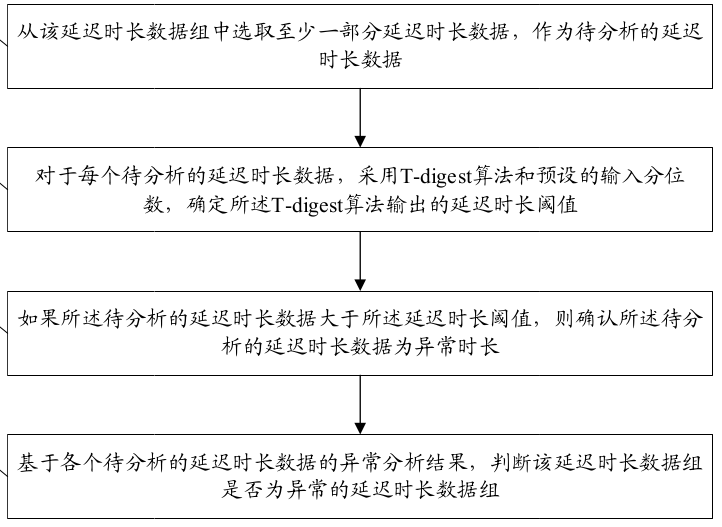
\includegraphics[width=8cm]{img/z2.png}
	\bicaption{延迟前置过滤}{Lantency Pre-filter}
	\label{延迟前置过滤}
\end{figure}

以上实现的延迟判别方式仅作为一种参考,具体根据生产环境下的需求,也可以关闭过滤操作以换取运行时计算量的降低,换取完整的日志保存,也可以使用其他的算法来进行异常判别,条件允许甚至可以包括深度学习技术的使用,其本质上相当于一个运行在日志提交进程上的插件,可以自主的修改,开启,和关闭。由于本文中所提到的方式主要用于减少嵌入式环境下的日志写入次数,只需要保留用于评估可靠性和稳定性的日志部分,因此使用了上述的工程实现。

\section{本章小结}
本章主要描述了基于\ref{计算机视觉算法的延迟观测}所描述的设计,如何实现一个面向计算机视觉算法部署的轻量级延迟观测系统。从延迟的观测事件如何产生开始,讨论了延迟的阶段选择如何实现,以及包含元数据的信息如何生成,并具体分析了这种实现方式具有较高性能水平的原因,以及如何去兼容和适应包括国产硬件在内的不同设备。最后还叙述了高性能日志系统的实现,以及如何通过设计定制的格式和前置过滤,优化日志系统的IO负载。整个系统可以切分为延迟观测装置,和信息记录装置两个部分。

延迟观测装置的实现中,通过编写了一个额外的框架,把对延迟信息的捕获和分析和SDK业务代码解耦,实现了相对更灵活,性能优秀的延迟及元数据捕获,在此总结对比了论文基于BPF实现的延迟观测系统实现的主要特性。

\begin{table}[htbp]
	\centering
	\bicaption{对比代码注入日志方式}{Compare the methods of log code injection}
	\label{对比代码注入日志方式}
	\begin{tabular}{ccc}
	\toprule
	   & 代码注入的日志记录 & 论文基于BPF实现 \\
	\midrule
	观测能见度 & API提供 & API提供,对内核更友好\\
	观测维度   & 受限  & 元数据hook,跨多环节  \\ 
	触发负载 & 无 & epoll \\
	时间戳获取 & 系统调用 & BPF \\
	元数据获取 & 多次进入内核态 & 一次进入内核态 \\
	可定制性 & 可定制性质弱,不适合工程化二次开发 & 解耦合,可编程性强\\
	安全保证 & 无 & LLVM提供 \\
	\bottomrule
	\end{tabular}
\end{table}

\begin{table}[htbp]
	\centering
	\bicaption{对比硬件支持的性能分析工具}{Comparing performance analysis tools supported by hardware}
	\label{对比硬件支持的性能分析工具}
	\begin{tabular}{ccc}
		\toprule
		& 硬件支持的性能分析工具 & 论文基于BPF实现 \\
		\midrule
		观测能见度 & 硬件自身更高 & 取决于硬件API,操作系统数据更友好\\
		观测颗粒度   & 函数符号,更细  & 模块,取决于封装程度  \\ 
		性能负载 & 高,不能用在实时场景 & 低,可用在运行时观测 \\
		可定制性 & 不可定制,通过GUI使用 & 解耦合,可编程性强\\
		安全保证 & 工具自身保证 & LLVM提供 \\
		\bottomrule
	\end{tabular}
\end{table}

信息记录装置的实现中,因为需要用于长时间的运行时监测,因此实现时力求减少性能开销,以适应计算机视觉算法部署这类内存和计算资源紧张的边缘计算场景,围绕原生异步IO和BPF获得信息方式的特点,进行了一系列的工程优化,和延迟观测装置衔接后较好的满足了持久化需求。

\chapter{边缘计算场景下的延迟观测实践}

正如在\ref{计算机视觉算法延迟的提取方式}中的描述,延迟采样的具体方式,以及如何利用延迟本身以及元数据,取决于框架的实现方式及面对的硬件场景。但出于商业数据隐私保护等原因,整个延迟观测框架实质上依附于公司内部非开源实现的SDK,不便公开使用,因此实践部分主要以仿真为目的,重点在于体现延迟观测系统的效果和思路。实验的设计主要是抽离了框架的一部分实现,在简化的硬件平台和计算机视觉算法任务上实现了延迟观测。

\section{交通任务下的边缘计算场景}
\begin{figure}[htbp]
	\centering
	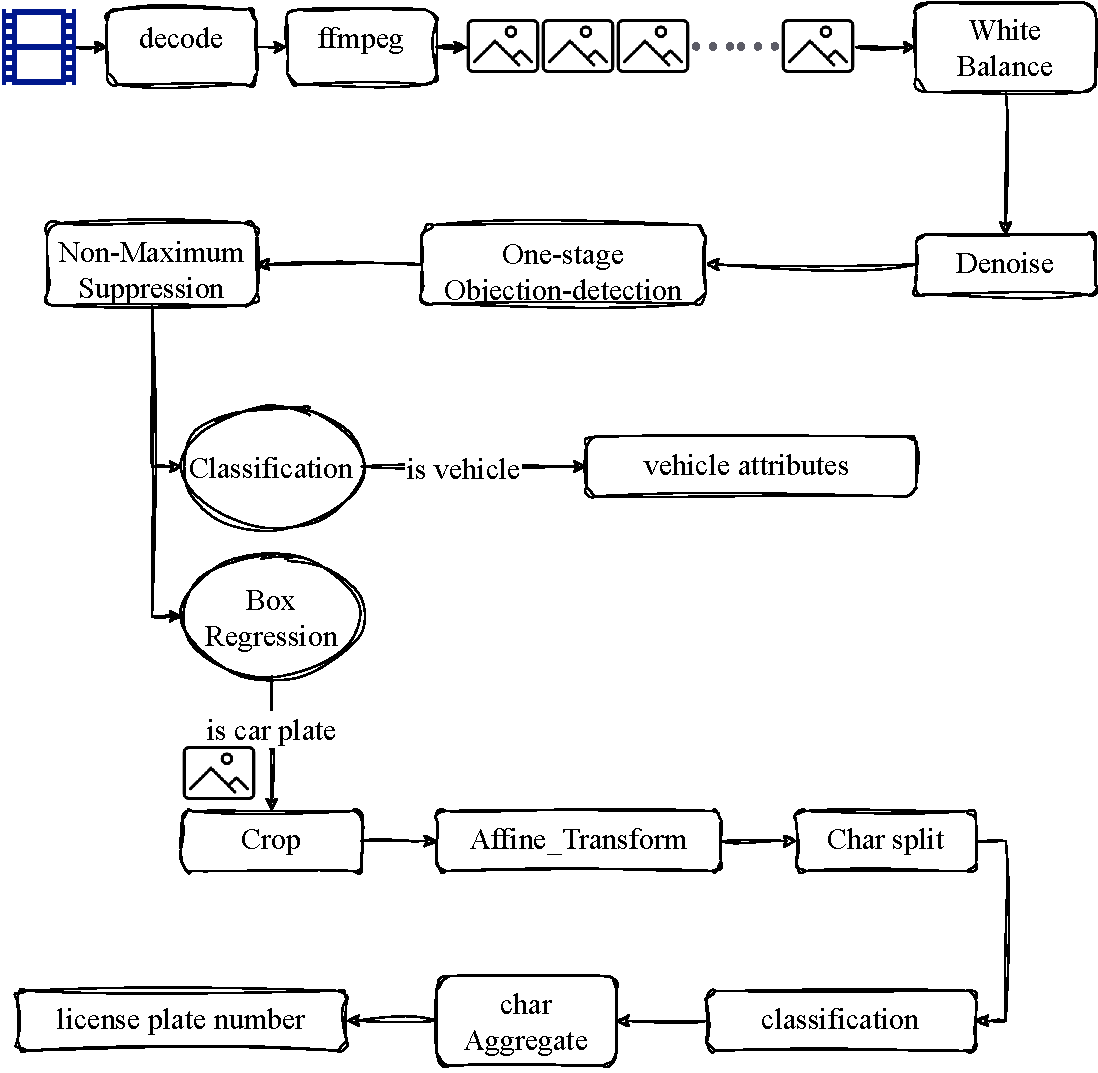
\includegraphics[width=12cm]{img/exp.pdf}
	\bicaption{简化的车牌识别流程}{Simplified Vehicle Plate Recognition Workflow}
	\label{简化的车牌识别流程}
\end{figure}
实验设计以一个车辆识别任务为例,其主要目的为从监控中获取数据,然后生成两个信息,分别为车辆的属性和车牌识别信息,产生的结果需要汇总提交给一个数据库中台,这是一个真实业务模型的简化。相比于一般的单模型算法,车牌的OCR(Optical Character Recognition)包含两个推理模型需要执行。图中车辆识别的属性内容(Vehicle Attributes),真实场景下可能还要做进一步的识别,在此处做了省略,只需要直接的分类结果即可。在第一阶段的识别过程中,会找到对应车牌的框体,并根据角点的位置进行裁剪,经过处理之后,由识别模块逐个识别字符内容,聚合(Char Aggregate)之后构造车牌号(License Plate Number)。对于部署外环境的,主要简单仿真了无线WIFI和有线传输两种方式,真实的视觉算法业务场景往往更加复杂,本文的主要内容是设计和讨论一种算法部署场景下的延迟观测实现方式,实验仅作为一种体现流程的方式。

\section{实验软硬件}
实验的主要设备瑞微芯公司的rk3588s,其目前的软件平台rknn2开发周期尚且较短,很多功能的实现可能存在偏差,兼容性和稳定性的探索也是社区正在进行的内容,本章主要内容是介绍实验的使用的软硬件规格,作为后续仿真实验的参考。

\subsection{信号来源}
\begin{figure}[htbp]
	\centering
	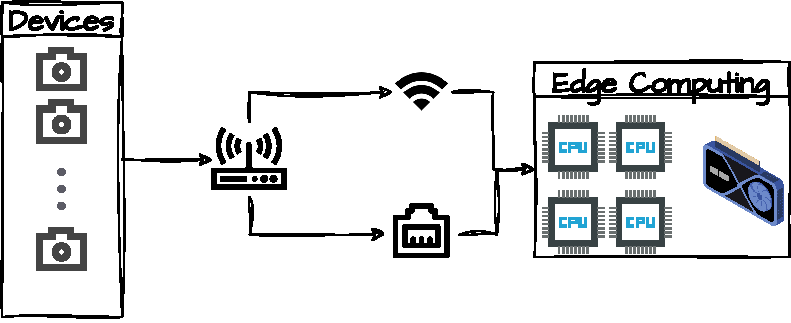
\includegraphics[width=8cm]{img/sim.pdf}
	\bicaption{实验仿真的传输场景}{
		Transmission Scenarios for Experimental Simulation}
	\label{实验仿真的传输场景}
\end{figure}
视觉算法在部署中,一个重要的部分是IO模块负责处理的信号传输。论文的实验仿真观测了两类常见的传输延迟,分别基于有线网络和无线网络。发送端为一台以无线方式连接到路由器的PC,接收端为一块开发版,同时使用有线网络和无线网络两种接受方式,有线接口为千兆网口(1000Mbps以太网),此处需要额外补充,虽然无线网卡支持WIFI6,但路由器不支持,实际是WIFI5的传输方式。

\subsection{部署开发板参数}

\paragraph{CPU}实验使用的开发板Orange Pi 5采用了瑞芯微RK3588S新一代八核64位处理器,具体为四核A76+四核A55,基于三星8nm,理论上设备驱动支持对所有硬件进行定频,实际考虑由于整个环节无法处理散热,板载空间较小,大核心并不能稳定在官方描述的2.4Ghz的水平,小核心低于1.8Ghz。

\paragraph{内存(RAM)}8LPDDR4x的规格,内存频率1Ghz。

\paragraph{NPU}6Tops算力的AI加速器,此处限定为INT8的算力而非浮点算力,和GPU不可直接类比。

\paragraph{存储}使用了一块三星的870EVO作为固态存储,还有一块TF卡为闪迪128G的规格,但开发板只支持PCIE2.0。

\paragraph{操作系统}Debian11,内核版本为5.19。

\paragraph{编译器和语言}由于BPF生态依赖于LLVM编译器,因此整个系统的编译均使用Clang/Clang++14,设定C/C++标准为C11和C++20。

\section{实验计算图表达}
\subsection{Taskflow}
本文所描述的计算视觉算法,模块间的并发和并行依赖于通过计算图的抽象方式。公司方面的商用SDK独立实现了这一计算图的调度和运行部分的功能组件,但出于保密等原因不便使用。论文所选用的简化实现是目前C++开源社区一个相对具影响力的开源的任务编排引擎TaskFlow\cite{huang2019cpp}。

这一框架的主要目标是简化异步任务处理的复杂性,使得开发人员可以更轻松地编写可维护的代码,支持跟踪每个任务的状态,以及它们的依赖关系和执行顺序,通过任务调度器安排任务的执行顺序,并处理任务之间的依赖关系。同时支持多种后端存储,包括内存、文件、数据库等,可以满足实验的测试需求。

\subsection{简单的模块封装}
模块主体分为5个类别,IO模块,前处理(Pre-Process)模块,后处理(Post-Process)模块,推理模块,以及负责一些辅助功能的其他模块。
\subsubsection{IO模块}
论文的实验环节仅做简单模拟,没有直接进行真实的视频流采集,直接从图片阶段开始。IO模块主要用于边缘设备端,接受从另一侧发送过来的图片数据。主要作用为转发图片到之后的模块,和对实时数据进行简单的缓存缓存,等待之后的模块完成图像分析后。

\subsubsection{前处理模块}
\begin{figure}[H]
	\centering
	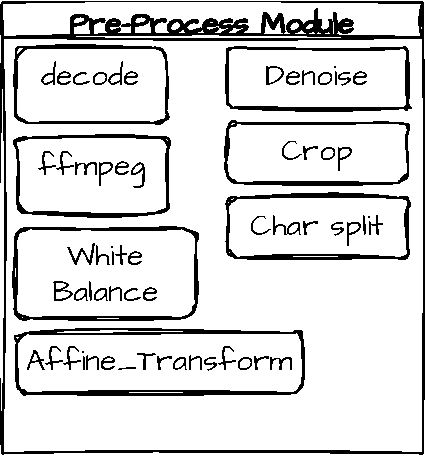
\includegraphics[width=8cm]{img/m1.pdf}
	\bicaption{前处理模块汇总}{Summary of preprocessing modules}
	\label{前处理模块汇总}
\end{figure}
\paragraph{解码(Decode)和ffmpeg}
视觉算法前处理的模块用于数据推理前,对于解码(decode)用于对输入的视频信号进行解码,ffmpeg实际常用于对视频流进行切分,用于将视频逐帧分为单张图片,实验中并未使用视频信号,因此在模拟中不会实现。

\paragraph{去噪(Denoise)和白平衡(White balance)}

由于图像质量容易受光照、天气、相机位置等因素的影响,所以在识别车牌之前需要先对相机直出图像做一些预处理,对后续识别提供辅助。一般会根据对现场环境和已经拍摄到的图像的分析,实现相机的自动白平衡处理等,并对图像进行噪声过滤、对比度增强等。

论文中仿真中简单封装了两个简单的算法,模拟实际场景的部分计算负载。其中白平衡采用基于直方图的白平衡算法(Histogram-based Algorithm),该算法使用直方图来计算每个通道的像素数量,并对每个通道进行缩放,以便使所有通道的像素数量相等。这样可以将色彩平衡应用于整个图像。去噪部分则使用了双边滤波器(Bilateral Filter),该算法可以平滑图像,同时保留图像的边缘信息。双边滤波器结合了空间滤波和灰度值滤波,可以有效地去除高斯噪声和保留图像的细节。如果涉及到更具体的部分,例如需要考虑特殊气象条件的去雾等环节,和论文主旨已经关系不大,因此做出了简化,只保留了两个基础的前处理。

\paragraph{切割(Crop)}
对车牌的识别首先会根据目标检测模型所得到的Bounding Box,裁剪出车牌对应的位置,将不相关的背景信息去除,减少信息的干扰和内存占用,降低计算的复杂度,提高识别的速度。

\paragraph{仿射变换(Affine-Transform)}
由于拍摄角度的原因以及车辆在行驶中会发生倾斜或抖动,导致拍摄到的车牌图像不水平或不垂直,这会影响车牌字符的分割和识别。因此,通过对车牌图像投影变换,可以改善图像质量,提高字符分割和识别的准确率,\verb*|Affine_Transform|的模块即对应这一实现,具体参数设置一般依赖于角点的位置信息。

\paragraph{字符分割(Char Split)}\label{字符分割}
常规的字符识别,最基础方法是二值化处理后,通过寻找连通区域来确定字符的位置。连通区域是指相邻像素值相同的像素构成的区域,可以通过遍历像素来检测连通区域,然后将连通区域分割成单个字符。但由于车牌本身是一种具有较强先验知识的识别对象,已知字符大小基本一致,且不考虑图像形变位置固定,因此更常用的是基于垂直投影的字符分割算法,通过对每一列的像素值进行投影来检测字符的位置。字符与字符之间的空白区域会导致投影值较小,根据投影值的变化来完成字符分割。


\subsubsection{后处理模块}
\begin{figure}[H]
	\centering
	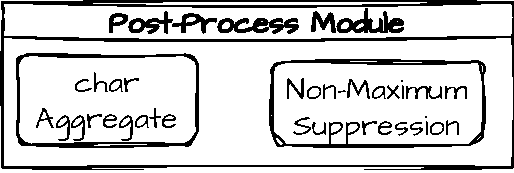
\includegraphics[width=8cm]{img/m2.pdf}
	\bicaption{后处理模块汇总}{Summary of postprocessing modules}
	\label{后处理模块汇总}
\end{figure}
\paragraph{非极大值抑制(Non-maximum suppression)}
NMS是目标检测中常用的一种算法,用于去除重叠的检测框,保留最终的目标框。其基本思想是在检测结果中,保留置信度最高的目标框,并剔除与其重叠度较高的目标框。主要步骤是按照置信度(confidence)进行排序,然后选择置信度最高的目标框作为基准框,并将其余的框中与基准框的IOU(Intersection over Union)小于等于一定阈值的重叠框不断迭代删除。

在目标检测算法中,NMS算法常被视为一个后处理的性能瓶颈环节,但细化的实现有较多区别。例如有的算法处于效率和并行度考虑,用了MaxpoolNMS等适合并行的方式,也有类似于Soft-NMS(应用于YOLOV7)等更多考虑场景下的优化,使用软阈值方法,不是直接剔除重叠框,而是通过减少其置信度的方法来减小其在后续处理中的影响,更适合密集目标检测和遮挡情况的算法。

\paragraph{字符聚合(Char Aggregate)}
本文对字符的识别是通过分割源图像后,单个执行分类,因此还需要进行一个额外的聚合,重新生成车牌信息,这属于服务于业务逻辑的后处理模块。



\subsubsection{推理模块}
\begin{figure}[H]
	\centering
	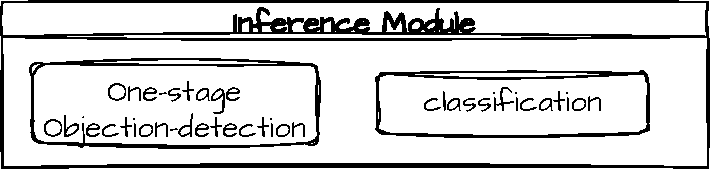
\includegraphics[width=8cm]{img/m3.pdf}
	\bicaption{推理模块汇总}{Summary of inference modules}
	\label{推理模块汇总}
\end{figure}
实验使用的目标检测模型来自百度paddlepaddle的模型库,字符识别采用公司自有分类模型。RKNN平台是一种专门为神经网络计算优化设计的平台,提供了针对瑞芯微自家的处理器进行优化的神经网络推理引擎,使得在嵌入式设备上运行的神经网络模型能够以更高的效率和更低的功耗完成推理任务。由于硬件平台的NPU为定制化的ASIC硬件,因此需要依赖于ONNX(Open Neural Network Exchange)的中间表示,把有一般框架(Tensoflow,pytorch,paddlepaddle etc.)模型的转化成RKNN支持的格式。

\subsubsection{其他模块}
\paragraph{序列化(Serialization)}
序列化的主要任务是将之前获得的车牌信息和车辆属性,以特定的格式组合起来,本实验中使用的方式为protobuf,是Google公司开发的一种轻量级、高效的数据序列化格式,用于在不同的计算机系统之间进行数据交换。

\paragraph{数据库事物提交(Database IO)}
数据库事物的提交是最后将内容写入数据库中存储的环节,需要等待事物完整执行后才能返回。本文实验所用的是一个运行在开发板上的MySql8.0。


\section{延迟观测的具体方式}
\subsection{延迟阶段划分}
\ref{简化的车牌识别流程}中描述了整个算法的流程,在进行延迟的观测前,首先应该进行阶段的划分。以完整的观测而言,图片的数据路径可以参考性的划分为以下没有重叠路径的阶段。

\paragraph{传输阶段}
\begin{figure}[H]
	\centering
	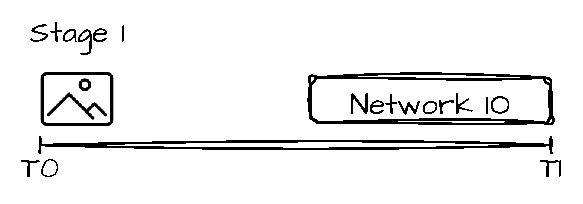
\includegraphics[width=8cm]{img/s1.pdf}
	\bicaption{传输阶段}{stage of transmission}
	\label{传输阶段}
\end{figure}
此阶段描述通过有线或无线网络接受的图片数据,其延迟包括发送端到路由器,路由器再通过Wifi和有线网络传输到Network IO模块的延迟,由于两部分处于不同的设备,因此需要考虑时钟的校准,注意$t_0$的时间应来自于RPC中的参数,无法通过BPF直接获得。


\paragraph{目标检测前处理}
\begin{figure}[H]
	\centering
	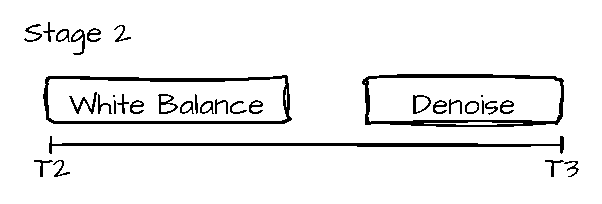
\includegraphics[width=8cm]{img/s2.pdf}
	\bicaption{目标检测前处理阶段}{stage of object detection pre-processing}
	\label{目标检测前处理阶段}
\end{figure}
视觉算法前处理的模块用于数据推理前,解码(Decode)用于对输入的视频信号进行解码,ffmpeg用于对视频流进行切分,将视频逐帧分为单张图片,实验中并未使用视频信号,因此在模拟中不会实现。

\paragraph{目标检测}
\begin{figure}[H]
	\centering
	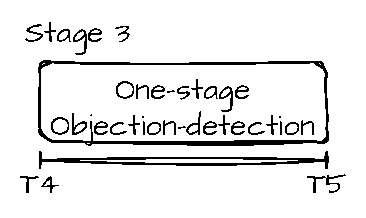
\includegraphics[width=8cm]{img/s3.pdf}
	\bicaption{目标检测阶段}{stage of object detection}
	\label{目标检测阶段阶段}
\end{figure}
此阶段执行目标检测模型,是核心的推理部分,具有最长的延迟,时间即为板载内存和NPU进行数据交互以及完成计算的时间。

\paragraph{目标检测后处理}
\begin{figure}[H]
	\centering
	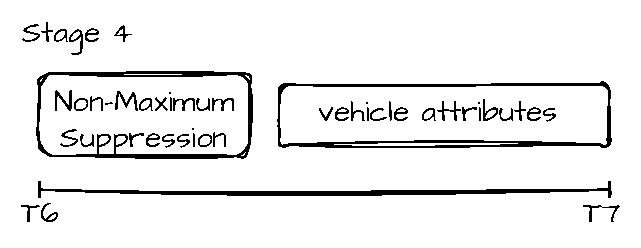
\includegraphics[width=8cm]{img/s4.pdf}
	\bicaption{目标检测后处理阶段阶段}{stage of object detection post-processing}
	\label{目标检测后处理阶段阶段}
\end{figure}
目标检测的后处理主要为通过NMS算法筛选车辆和车牌的候选框,车辆候选框有对应的分类数据,虽然one-stage模型输出的分类是一个概率分布,但一般softmax类似的操作都会直接装载在模型内部,此处会被直接序列化为车牌属性信息。

\paragraph{车牌识别前处理}
\begin{figure}[H]
	\centering
	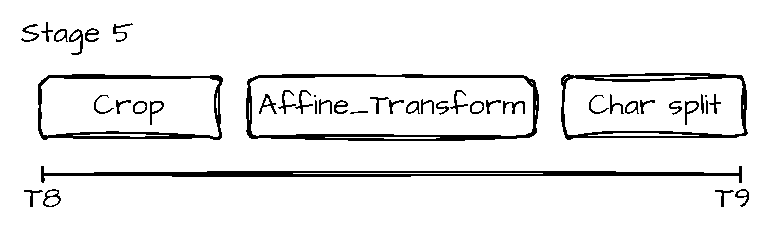
\includegraphics[width=8cm]{img/s5.pdf}
	\bicaption{车牌识别前处理阶段}{stage of 
		vehicle plate recognition pre-processing}
	\label{车牌识别前处理阶段}
\end{figure}
车牌识别的前处理会先利用目标检测中,分类为车牌框的边界角点,对原图进行裁剪,产生新的图像。这一图像先利用关键点检测等方式,对倾斜变形进行修复,最后利用\ref{字符分割}中的算法切分为多张小图,每张对应一个单独的字符。

\paragraph{字符识别}

\begin{figure}[H]
	\centering
	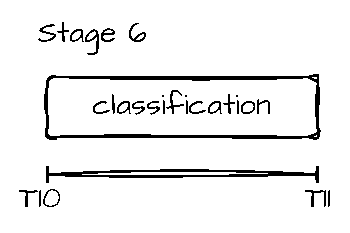
\includegraphics[width=6cm]{img/s6.pdf}
	\bicaption{字符识别阶段}{stage of char character classification}
	\label{字符识别阶段}
\end{figure}

此阶段是一个分类任务,因为不同于OCR,车牌的词典非常固定,因此推理模型的延迟通常远低于一般的OCR模型。字符识别模型需要执行多次,对每个切分的单字符图片均执行一次推理。


\paragraph{车牌识别后处理}
\begin{figure}[H]
	\centering
	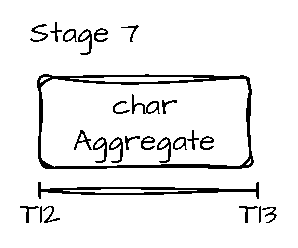
\includegraphics[width=6cm]{img/s7.pdf}
	\bicaption{车牌识别后处理阶段}{stage of 
		vehicle plate recognition post-processing}
	\label{车牌识别后处理阶段}
\end{figure}

多个字符结果需要进行聚合,生成对应的车牌信息。可能还需要进行一些额外的检查,这一部分的后处理相对简单。

\paragraph{信息提交}

\begin{figure}[H]
	\centering
	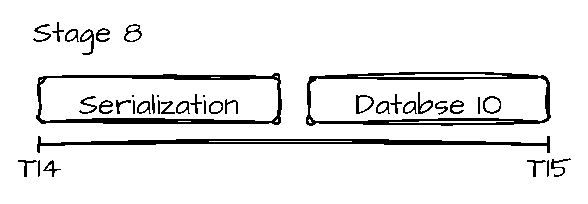
\includegraphics[width=8cm]{img/s8.pdf}
	\bicaption{信息提交阶段}{stage of information submission}
	\label{信息提交阶段}
\end{figure}

根据属性信息,和车牌信息,进行序列化之后,通过RPC向数据库提交,响应请求。此阶段的延迟同样取决于数据库的部署位置,实现方式多样化。

\subsection{观测结果选择}
上述阶段体现了全部车辆识别和车牌OCR任务过程中,一种可以参考的拆分方式。自定义拆分粒度的过程中,不一定需要按照上述方式,例如$stage_1$,$stage_2$,$stage_3$的内容其实可以合并,因为数据路径不存在重叠。但例如$stage_5$到$stage_6$的阶段,一张车牌图片被按照字符切分成了多组数据,则必须分离观测。

实验主要服务于展示观测效果,因此只选取部分。此处实验,选择
$stage_1$,$stage_3$,$stage_4$,$stage_5$,$stage_8$
其余部分略去。其观测日志的格式如下

\begin{table}[htbp]
	\centering
	\bicaption{实验观测日志的格式}{Comparing performance analysis tools supported by hardware}
	\label{实验观测日志的格式}
	\begin{tabular}{cc}
		\toprule
		条目(item)  & 对应阶段(stage) \\
		\midrule
		$stage_1$  & 传输阶段  \\ 
		$stage_3$  & 目标检测 \\
		$stage_4$  & 目标检测后处理\\
		$stage_5$  & 车牌识别前处理 \\
		$stage_8$  & 信息提交\\
		\bottomrule
	\end{tabular}
\end{table}

\section{利用观测结果指导优化}
\subsection{观测设备的硬件负载}
仿真实验环节的目的重点在于体现机制,而非具体服务于实际场景。因此实验中只保留了几个在嵌入式开发下几个较为有特色的元数据信息进行记录。
\subsubsection{内存使用率}
内存是嵌入式系统中非常重要的一个指标,内存不足会引发严重的性能问题,尤其嵌入式条件下,设备IO的性能不足,一旦触发SWAP会导致严重的服务质量降低。但过低的内存使用率代表没有充分硬件的性能,存在资源浪费,因此内存使用率是一个非常有用的观测指标。
\subsubsection{NPU负载}
\ref{延迟观测事件的信息获取}介绍了关于NPU的相关信息,RK3588S虽然理论上和RK3588仅有接口层面和封装尺寸的差异,但实际上"体质"(ASIC Quality)上略有区别,此系列所有都可以预先进行定频设置,理论负载为1Ghz,但其实可能受到各种因素的影响无法达到指定频率。

观测NPU的使用率,官方给出了一个NPU负载率的指标,取值范围在0-1之间,但目前文档中并未明确这一指标的具体计算方式,和NVIDIA的Nsight类似分析,可以准确定位具体是IO还是计算瓶颈的指令层面负载相比,尚无法提供较好的观测分析,只能作为一个分析的参考值。

\subsection{查找性能瓶颈}
\begin{figure}[H]
	\centering
	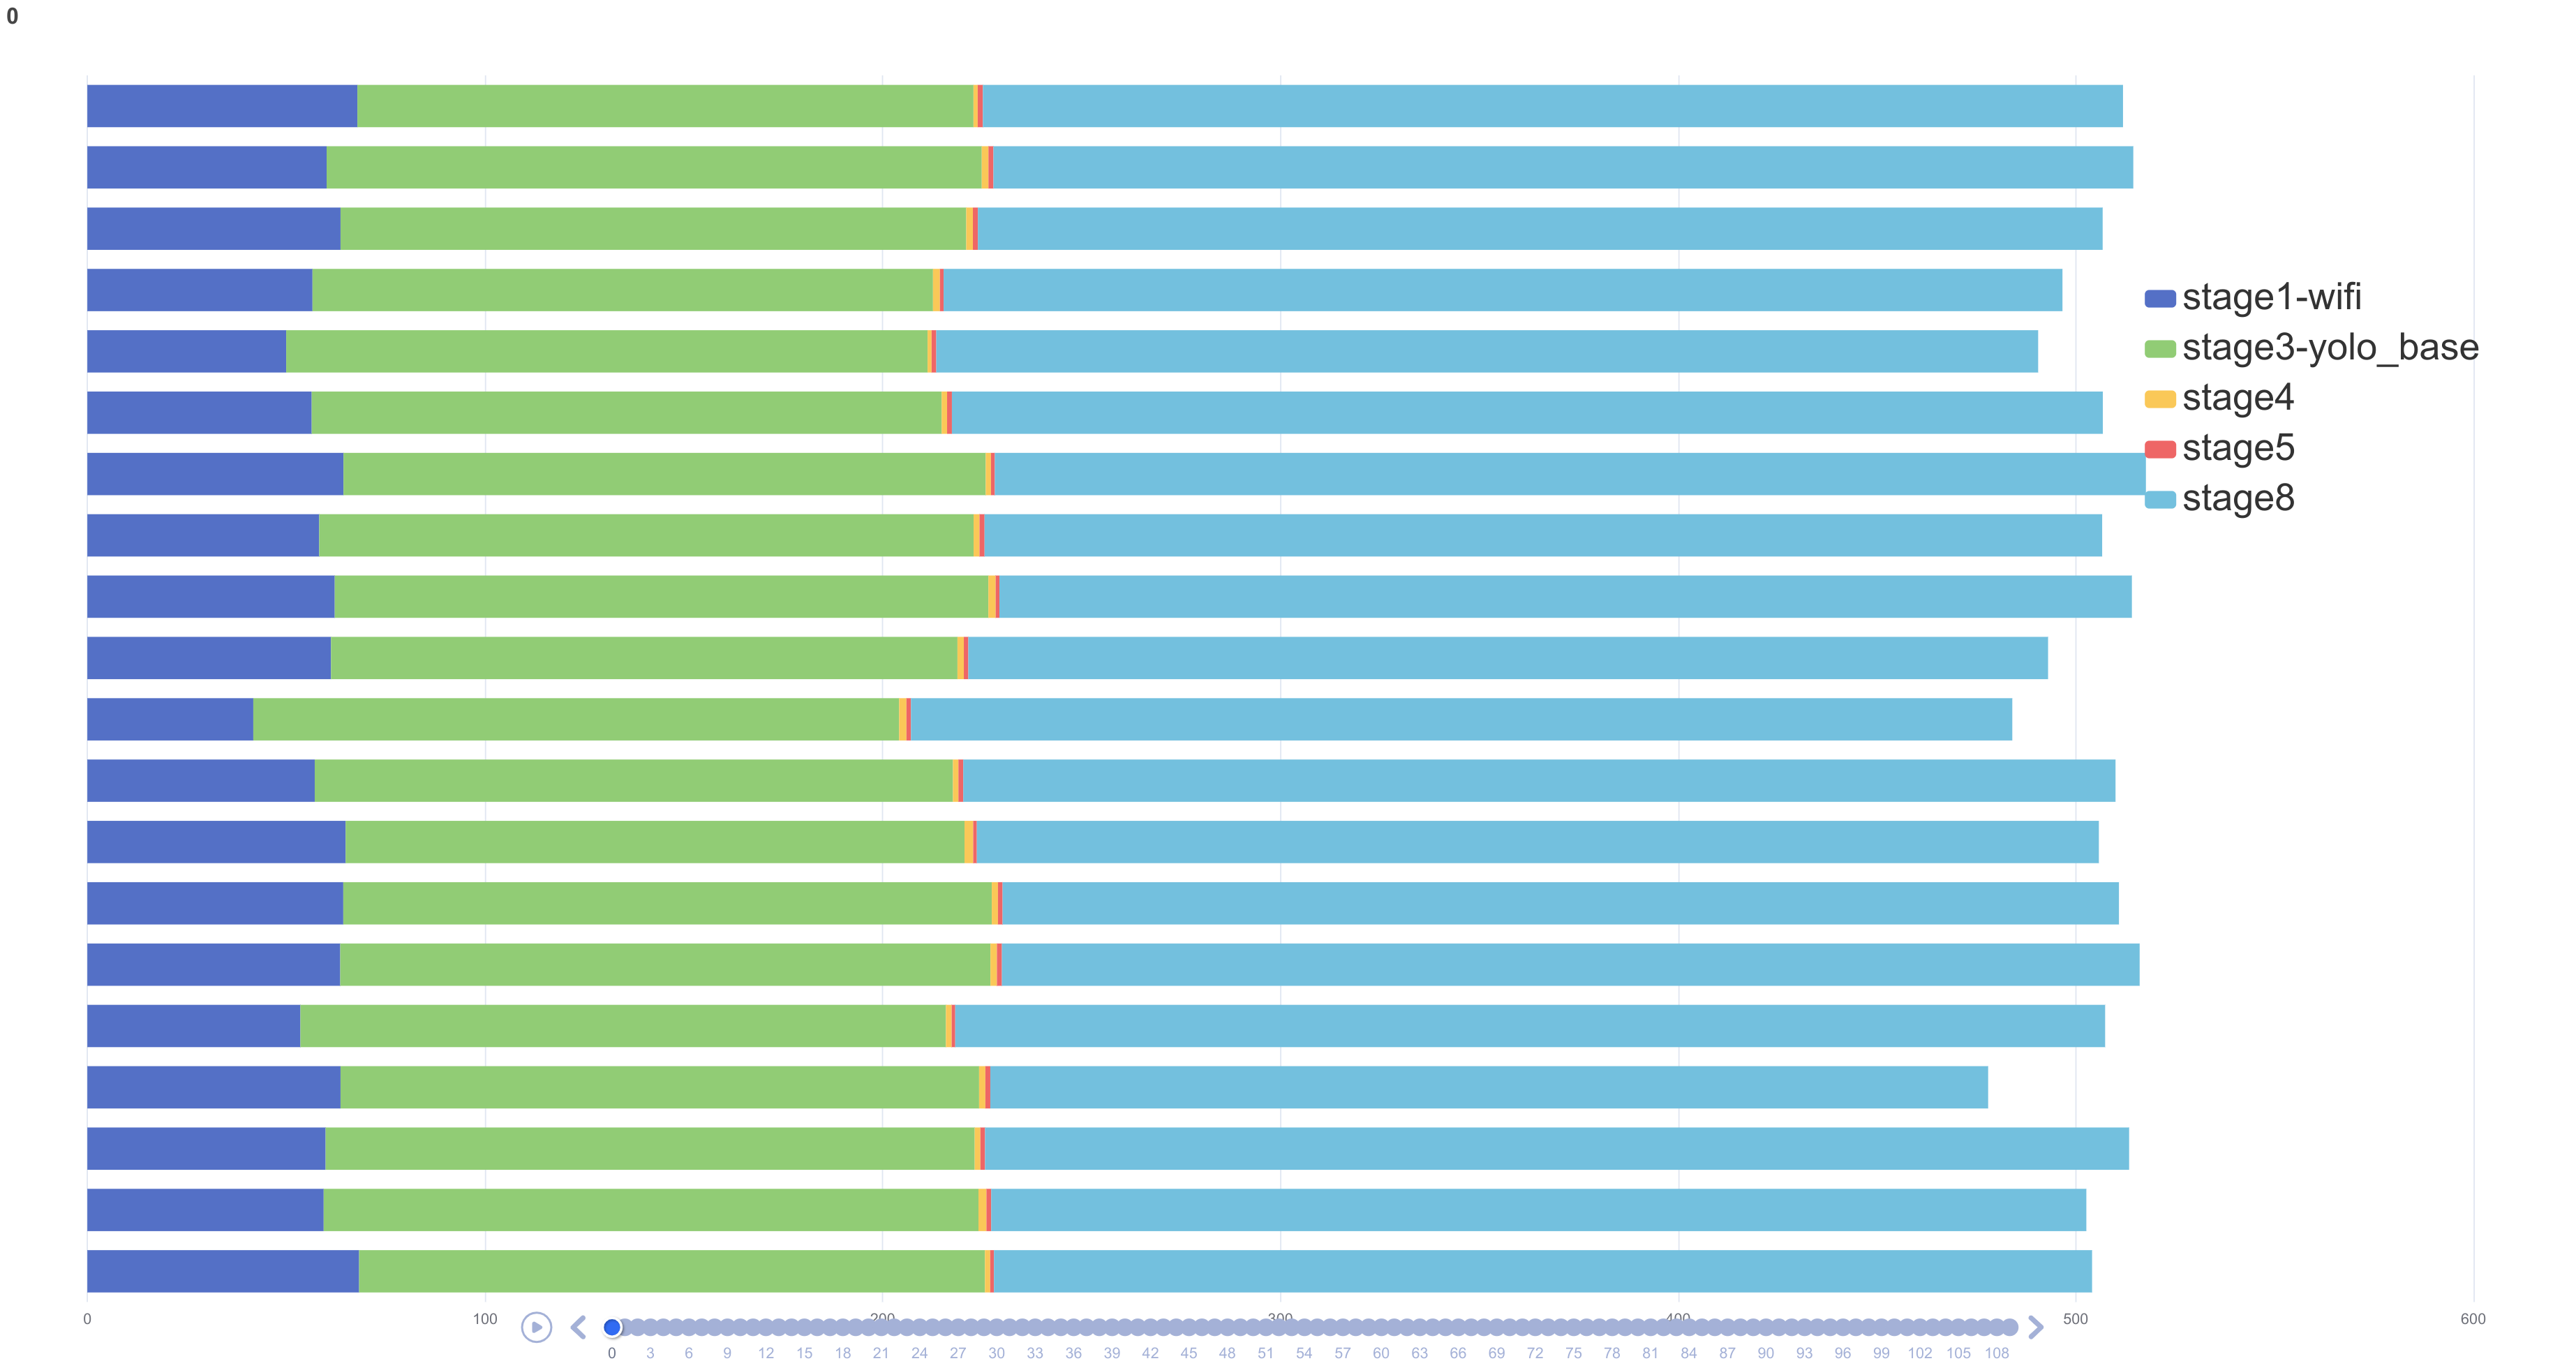
\includegraphics[width=15cm]{img/echarts.png}
	\bicaption{延迟阶段选择结果可视化}{Latency stage selection result visualization}
	\label{延迟阶段选择结果可视化}
\end{figure}

如图所示为前20张图像的推理过程中,对应\ref{实验观测日志的格式}阶段选择的延迟可视化结果。可视化框架通过echarts实现,相比平均值等统计指标在小数据规模下,能方便的展示各阶段延迟的比重,更便于发现推理过程中的优化点。

可以显著的看到,$stage_8$(浅蓝色块)的阶段占据了推理的主要延迟开销,显然是因为向数据库单次提交等待确认的开销太大,因此首先应该考虑优化这一部分。其次,$stage_3$(绿色块)则是模型One-stage目标检测的推理部分,$stage_1$为数据传输的延迟。

\begin{figure}[H]
	\centering
	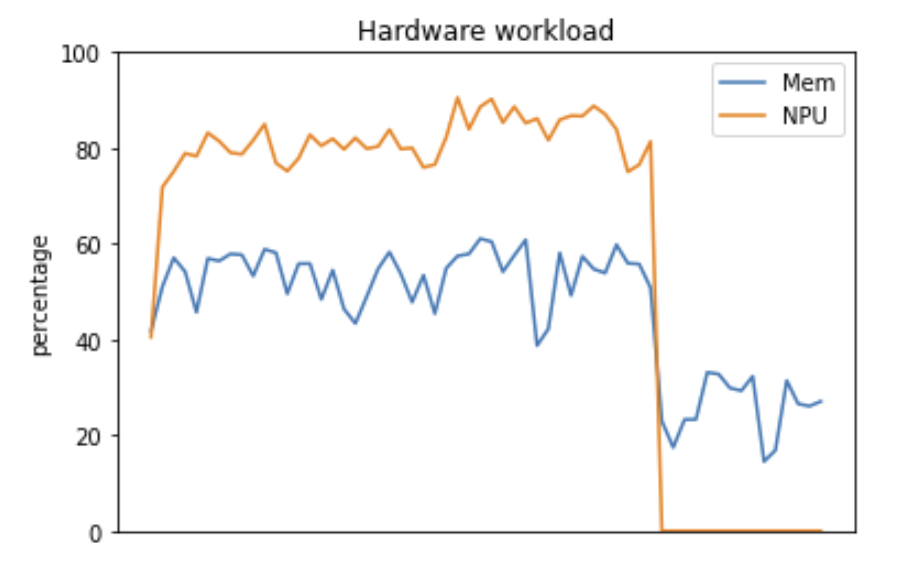
\includegraphics[width=8cm]{img/hw_c.png}
	\bicaption{内存/NPU使用率}{RAM/NPU usage}
	\label{负载曲线}
\end{figure}
查看此时内存使用率,处于较低的水平,因此我们可以考虑利用缓存机制,对数据库进行批量提交,以及构造连接池等方式,用内存换取延迟,这种实现较为复杂,不在仿真实验的范畴。


\begin{figure}[H]
	\centering
	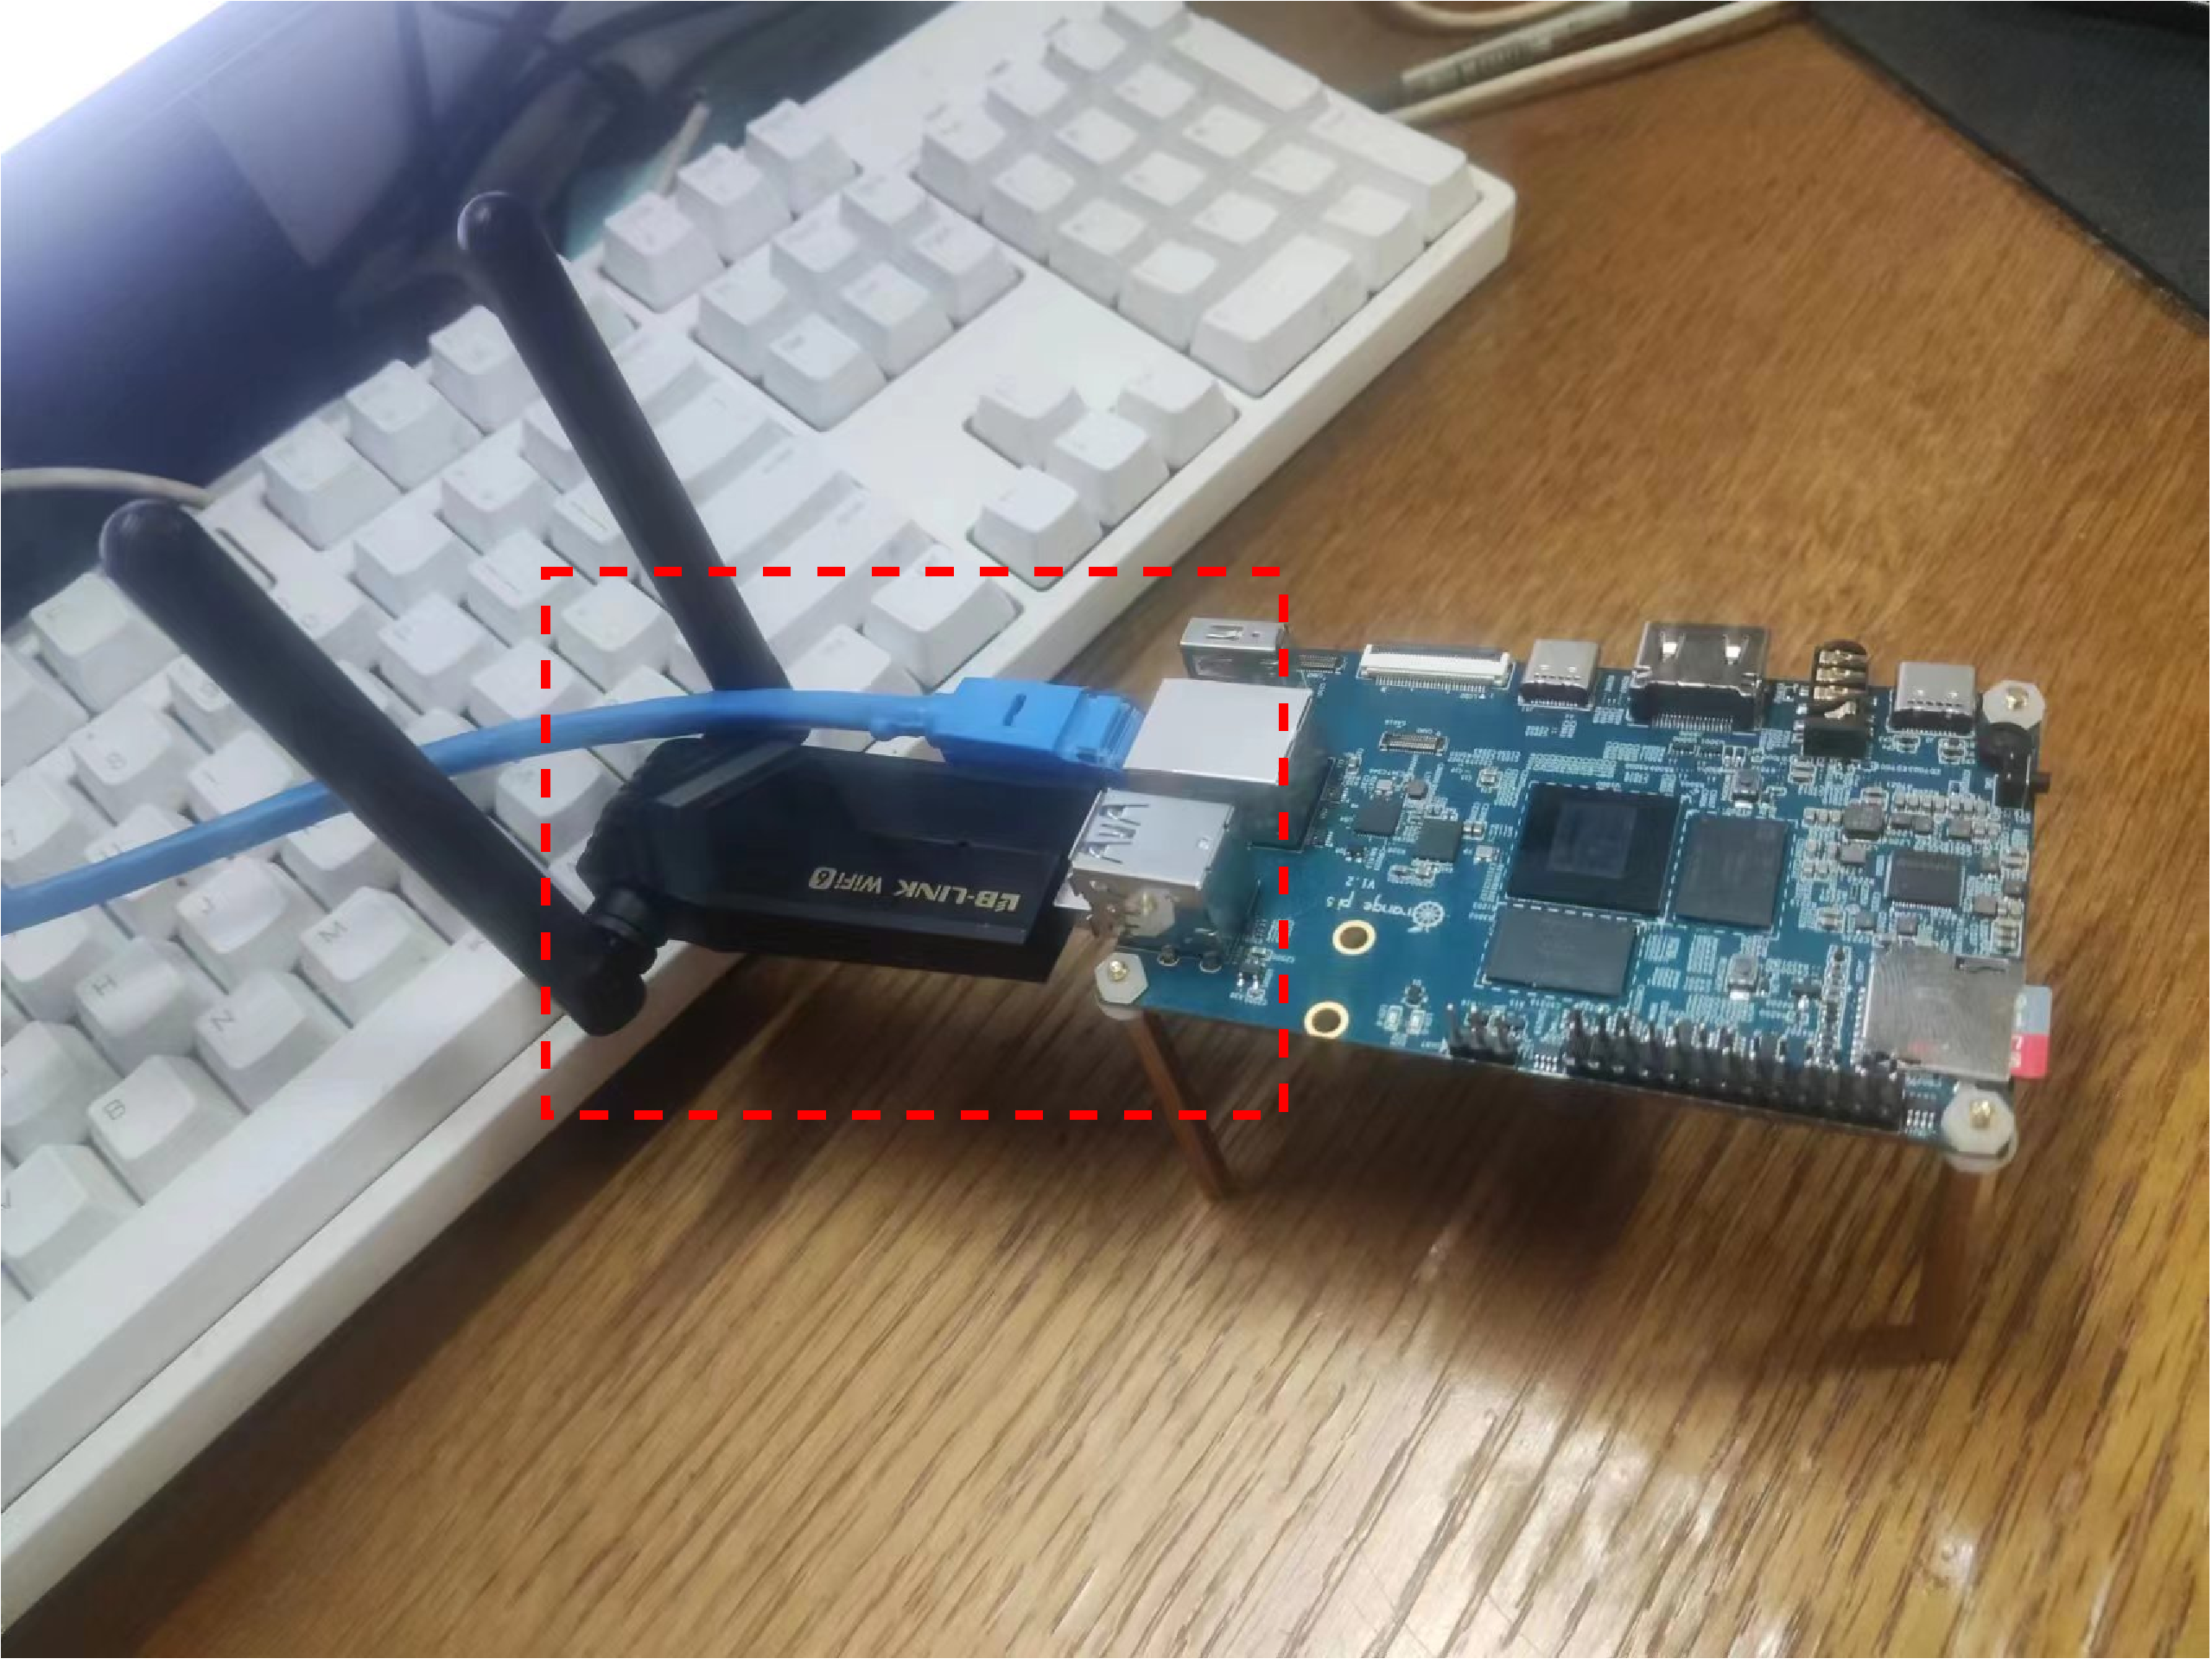
\includegraphics[width=8cm]{img/port.pdf}
	\bicaption{USB无线网卡接入和网线接入}{USB wireless network card access and network cable access}
	\label{网卡接入}
\end{figure}

就模型情况而言,更直接的办法是尝试选择将开发板从无线连接替换为有线(上图红色框),并将模型替换为最高性能的量化版本\verb*|yolov7tiny_8bit|版本,可以直观的体现优化效果。
\begin{figure}[H]
	\centering
	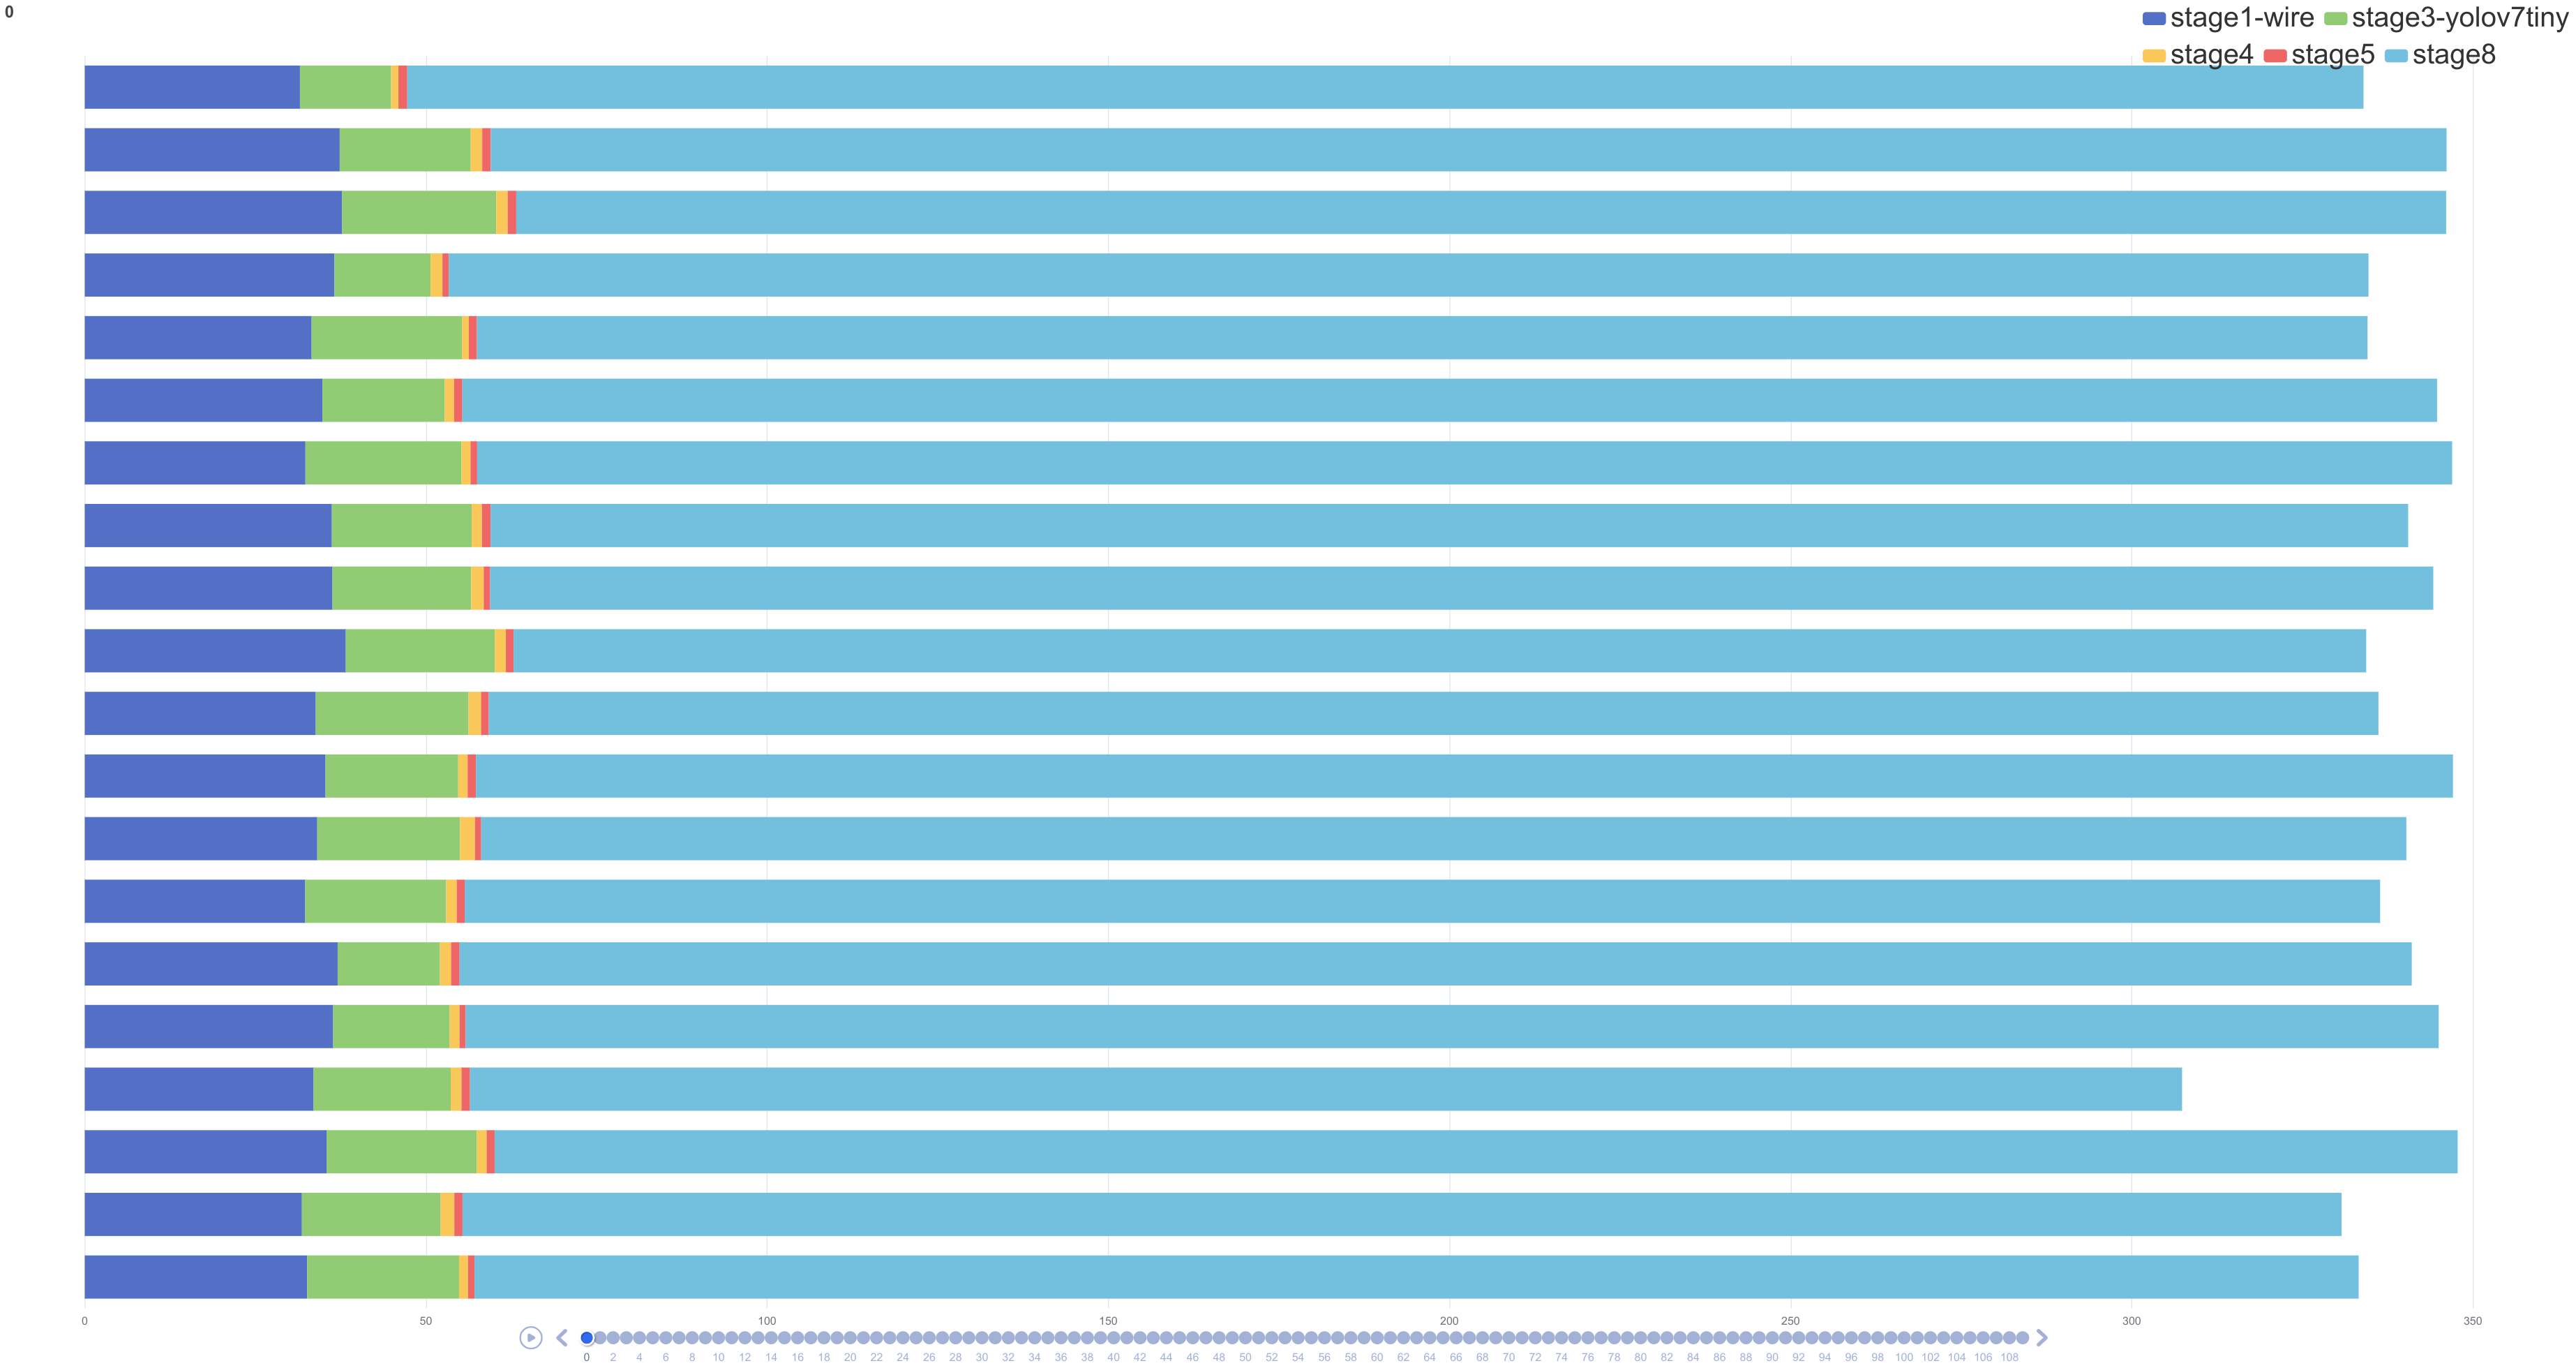
\includegraphics[width=15cm]{img/echarts2.png}
	\bicaption{优化后延迟阶段选择结果可视化}{Latency stage selection result visualization after optimization}
	\label{优化后阶段延迟}
\end{figure}
从结果可以看出,改善传输延迟和替换轻量级模型以后,$stage_1$(深蓝色块)和$stage_3$(绿色色块)和延迟在总体延迟中占比明显降低,通过这样的方式可以快速的选择可发现性能瓶颈,而不用修改算法代码本身,体现出了优秀的观测灵活度。


\subsection{快速对比量化模型替换后延迟}
严格来说,因为系统允许多线程的并行,因此例如网络等$stage_1$的延迟,实质上都被并发操作所重叠,真正的系统瓶颈在于模型推理,因为只能在单一硬件上计算,本质均为串行。真正维持较高负载水平的主要为NPU。

模型量化则是一种常用的加速方式,视觉算法的模型量化通常是指将一个深度学习模型的参数压缩为更小的表示形式,以减少存储空间和计算量,从而在边缘设备上实现更快的推理,量化(Quantization)指将模型中的浮点数参数转化为低位整数参数。通常使用的量化位数为8位或4位,可以显著降低模型的存储空间和计算量,但数据表示精度的降低,因此通常会对模型的准确率下降。真实部署中,我们经常希望在更换模型后,同时评估其对准确性的影响和推理延迟的效果影像,通常需要去直接修改部署的业务代码来打印日志,再编写单独的处理程序。

而基于上述可以快速进行阶段选择的独立延迟观测程序,我们可以只选择需要的阶段,例如针对目标检测阶段的模型,直接选择$stage_3$和$stage_4$,在不修改原代码的情况下实现快速对比量化后和更改模型后的延迟。

如图展示了基于基础的yolov7模型,替换为int8量化之后,以及进一步简化后的\verb*|yolov7tiny|模型,在RK3588设备上的推理延迟平均值,标注差,以及max/min值大小。

\begin{table}[htbp]
	\centering
	\bicaption{模型推理延迟数值}{Model inference latency value}
	\begin{tabular}{ccccc}
		\toprule
		模型  & 平均值(ms) & 标准差 & 最大值(ms) & 最小值(ms)\\
		\midrule
		\verb*|yolov7|          & 159.9 & 4.34 & 164.97 & 135.41  \\ 
		\verb*|yolov7_8bit|     & 80.99 & 3.38 & 84.99  & 63.74 \\ 
		\verb*|yolov7tiny_8bit| & 18.96  & 2.51 & 22.88 & 13.05\\ 
		\bottomrule
	\end{tabular}
\end{table}

\begin{figure}[htbp]
	\centering
	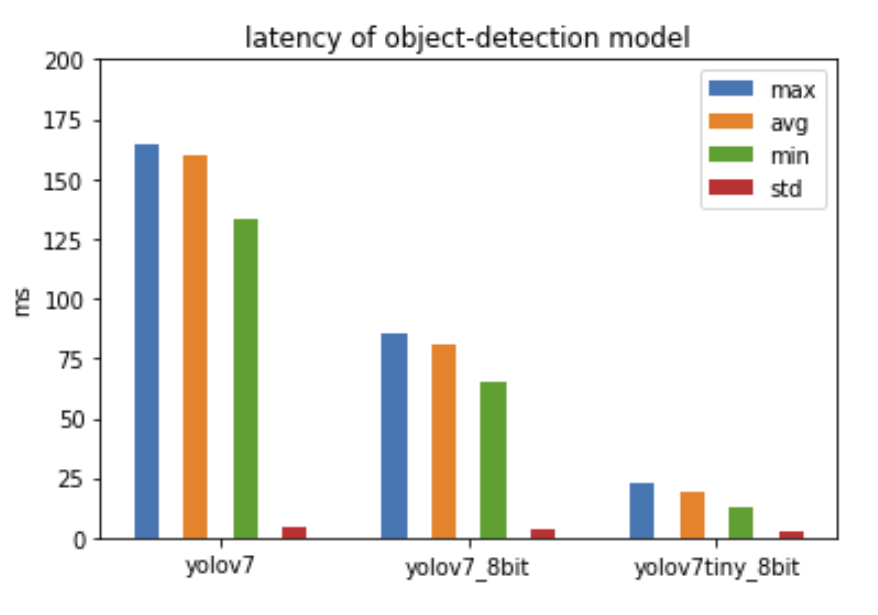
\includegraphics[width=8cm]{img/model.png}
	\bicaption{对比模型推理延迟}{Comparing model inference latency}
	\label{对比模型推理延迟}
\end{figure}

此处要说明的是,无论日志还是其他工具,并非不能统计上述结果,但都必须要修改业务代码本身,而论文实现的观测方法则只需要调整选择的配置即可,此处体现的主要优势在于观测的灵活性。

\subsection{使用前置过滤评估延迟的稳定性}\label{使用前置过滤评估延迟的稳定性}
\ref{基于T-digest的延迟过滤}延迟过滤机制,可以选择百分位点的具体数值,来适应不同波动率的数据。当延迟趋于稳定范围,则只有极端值会被记录,减少总体的日志IO次数。
\ref{实验仿真的传输场景}的可视化及统计结果,基本展示了运行时的发现优化点,快速测量指定阶段延迟的两种常用功能。

网络故障是导致延迟的常见原因。网络延迟增加一个最常见的例子就是,处于同一个网络下的某些设备互相发生带宽的争用,导致路由的负载不均匀,使得同一个无线局域网下,部分设备无法正常工作。论文在实验过程中仿真了这一情况,通过传输过程中,对将开发板所连接的无线网卡进行限速,将下行限制为\textbf{10Mbps}。

下图展示了推理输入2000张图片后,对开发板的无线网卡进行限流(Netrowk traffic control),之后再传输200张图片,整个推理的延迟的记录:
\begin{figure}[H]
	\centering
	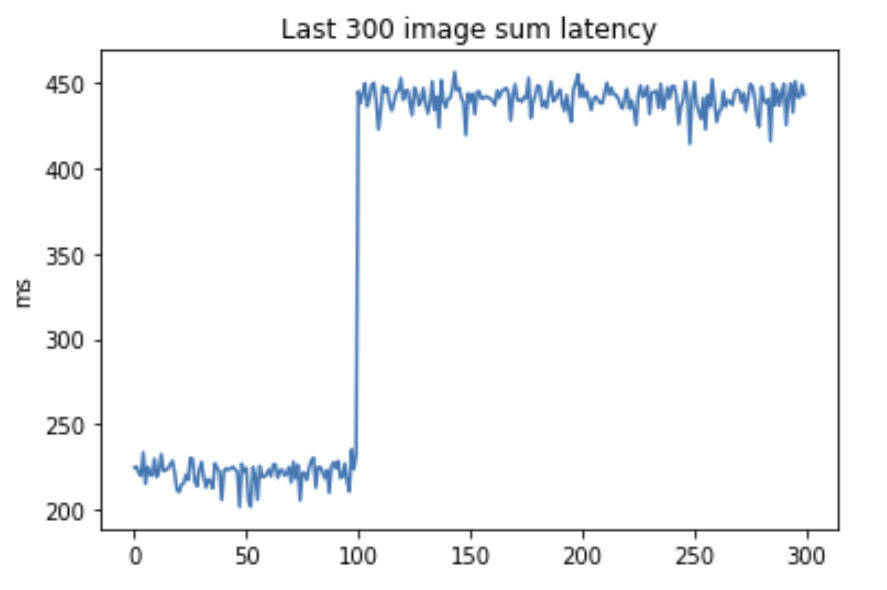
\includegraphics[width=8cm]{img/change.png}
	\bicaption{网卡限速后延迟变化}{Latency changes after wifi netrowk traffic control}
	\label{网卡限速后延迟变化}
\end{figure}

这一延迟的变化并非通过变点分析获得,而是通过\ref{延迟前置过滤的判定方法}描述的方式,查看日志记录次数的变化。
\begin{figure}[H]
	\centering
	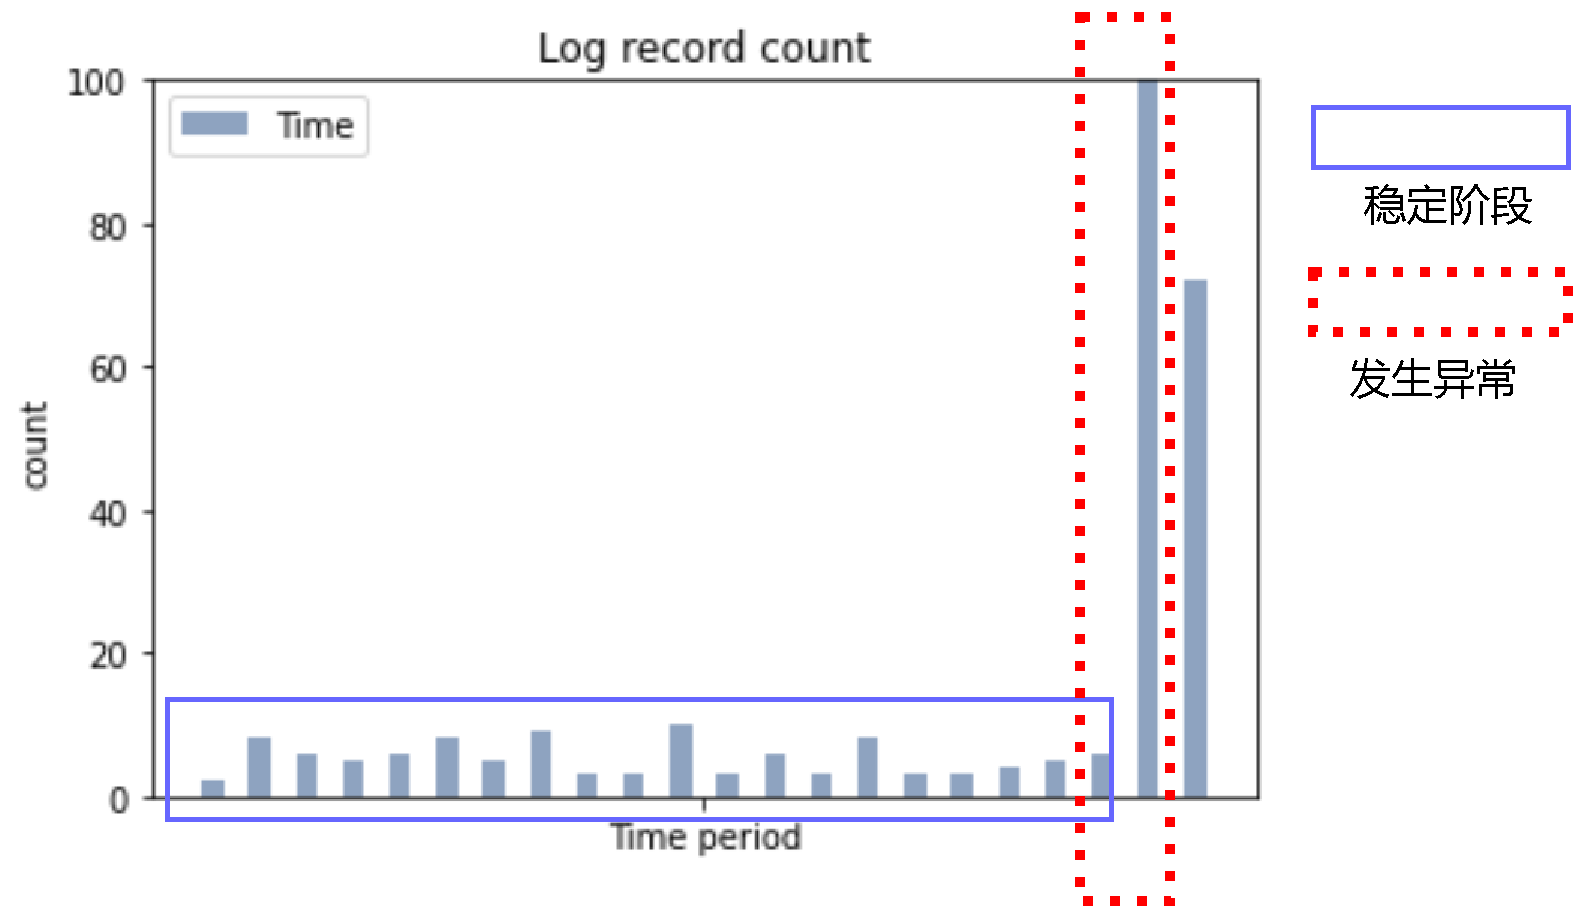
\includegraphics[width=8cm]{img/error.pdf}
	\bicaption{单位时间内延迟的记录次数}{The count of record per time period}
	\label{单位时间次数}
\end{figure}
蓝色框体即\ref{延迟前置过滤的判定方法}中的稳定阶段,代表输入的数据分布均匀,假设预设的分位数为$k$,只有在:
\begin{equation}
	latency \geq quantile(k)
\end{equation}
才会触发记录,红色框体则代表出现故障的时间点,此时由于网卡限流,导致数据的传输延迟快速增加,因此反复触发阈值条件,之后的一个周期T-digest算法的阈值被高延迟数据"稀释",记录次数下降,体现出了这种方式对数据分布的适应能力。

前文提到,由于不同的模块执行的稳定程度互有差异,因此算法对波动的容忍程度可以通过对于分位数的设定来改边,例如在日志记录的过程中,设定前置过滤所需要的分位数为\textbf{P95}和\textbf{P50}产生的过滤阈值如下:
\begin{figure}[H]
	\centering
	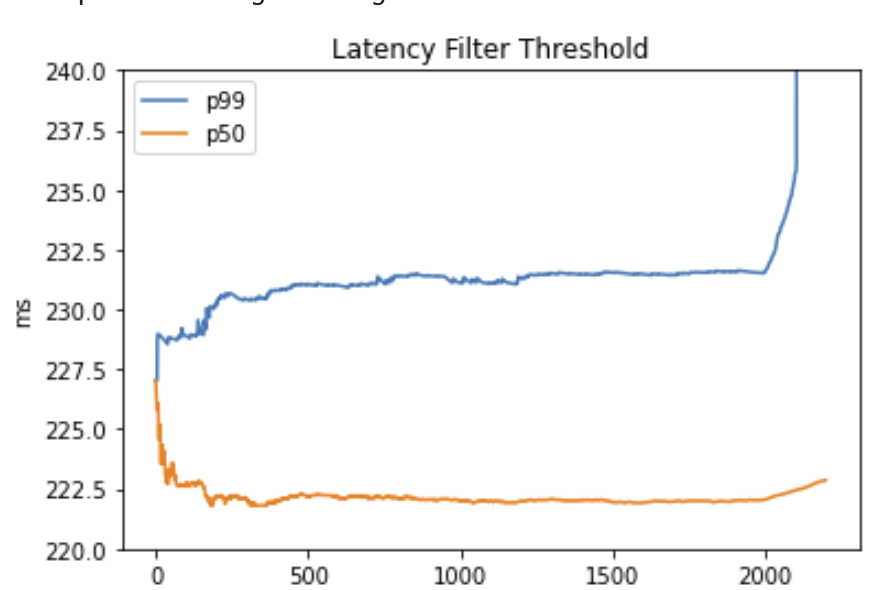
\includegraphics[width=8cm]{img/dp.png}
	\bicaption{不同分位数的过滤阈值}{Filter thresholds for different quantile}
	\label{不同分位数延迟的过滤阈值}
\end{figure}
如图所示,\textbf{P50}和\textbf{P95}都在一段时间的冷启动后,调整到了稳定的分布估计值,当网卡执行限流,延迟激增以后,高延迟数据影响更大的是后5$\%$的延迟分布情况,因此\textbf{P95}的敏感程度显然更大,变化更剧烈。当希望模块对延迟的波动监测更敏感,则应该设置更大的分位数,反之则减小。

\section{本章小结}
本章节在最新一代(2023年)的国产边缘计算硬件RK3588s上,对\ref{lantms}描述的基于模块的计算图视觉算法部署进行了实验性的仿真搭建,在一个简化的车牌车辆检测业务场景中,实践了\ref{轻量级视觉算法部署延迟观测系统实现}提出的轻量级延迟观测工具的,展示了主要功能和适用需求。
整体仿真实验从模块之间的数据关联,进行延迟阶段的划分出发,具体讨论了工具如何提高延迟测量的效率,快速评估推理过程性能瓶颈,以及前置延迟过滤装置进行事后追踪故障环节等功能细节,体现了方案特色及可行性。

\chapter{总结与展望}
\section{本文总结}
计算机视觉部署是一个需要兼顾效率和兼容性的工程问题,当放置到边缘计算的场景下,软硬件的实施会变得更加困难。出于优化和监测两种角度,都促使了对算法延迟观测的需求。然而传统的延迟观测方式依赖于日志注入,性能开销较高,且观测维度有效,硬件编译器使能的分析工具则因为沉重的图形界面,不仅缺乏可定制的能力,也不适合使用在用于运行时的场景。

本文通过运用近年来操作内核,包括eBPF模块在内的新特性,实现了一个服务于实际业务中针对计算机视觉部署SDK的延迟轻量级延迟观测系统,并探讨了在此方案下对不同部署硬件的兼容实现方式,主要研究成果如下

从设计选型和技术实现的角度,探讨实现了一种针对模块化计算机视觉算法部署场景的独立延迟观测程序,对比传统的基于日志的记录和采集方法,具有显著的灵活性优势,简化操作的同时,拓展了观测的维度和能见度。由于基于动态追踪的相关技术和理念进行设计实现实现,能通过按需采集的特性灵活调整观测负载,能较好的服务于边缘计算场景的于运行时观测,提供一定的故障发现和事后追踪能力。

实现了一个和观测程度相衔接的日志记录系统,以内核原生异步IO机制为核心,并通过设计固定格式的记录信息,和前置过滤装置来进行存储优化。具有低开销,低依赖的特点,和上述观测模块实现了良好的适配,共同构成了专利\cite{patent}内容。

因为日志记录部分和业务代码并无耦合,并适合衔接BPF程序的观测结果,经过改进后迁移到了内核IO的观测工具中 ,还作为开源项目提交到华为OpenEuler。
\section{下一步的工作展望}

自2021年以来,伴随半导体产业链的迅速发展,头部企业不仅在硬件参数上快速接近国际一流水平,于众多应用场景下实现了国产替代,并且软件生态方面也逐步成熟,开源社区活跃开发者不断增加,在包括以百度paddlepaddle,旷视天元等一众框架厂商的持续推动下,深度学习算法的部署逐步摆脱了中文场景下社区文档缺失,缺乏讨论解答的情况。

可观测性工具,是基础功能以外的需求。虽然并非直接作用于生产系统,但却是整个软硬件生态中不可获取的一部分,随着计算机神经网络模型,尤其是计算机视觉模型,从卷积神经网络到Transformer不断进化,参数膨胀的趋势显而易见。促使算力不断增长的同时,对部署性能也提出了更加苛刻的要求,这不仅需要芯片工艺架构方面的进步,更需要开发者在软件层面的优化和适配。但目前受限于实际情况,目前硬件的驱动厂商客观上暂时没有能力实现类似工具。

本文基于内核BPF等技术,讨论了一种针对深度学习视觉算法部署的延迟观测方案,对不同的推理硬件做了一定程度的兼容,是一种非常特化的可观测模块实现,受限于开发时间和本人水平所限,远未达到开箱即用的框架水平,仅满足了一部分的内部需求。但这也代表一种可能,即参照开源的标准,否能以类似MySql,Java,Node.js等知名项目一样,以统一的标准对外提供可观测接口,然后在开源社区的推动下,诞生例如\textbf{bpftrace}这样的项目,降低给开发者提供可观测能力的成本。作者由衷希望在未来,国产专用计算卡在软件生态领域,能达到今天NVIDIA的水平,使用者带来更多的便利。

\makebiblio
\backmatter
\begin{acknowledgement}
首先感谢学术导师范睿教授,企业导师朱政博士两位在学习和工作期间的指导,其次感谢上海科技大学校方提供了完善生活环境,以及各方面的培养资源。就研究项目而言,除了感谢芯翌科技公司的同事以外,特别需要感谢华为OpenEuler存储组的刘志强博士在开源社区的给予的帮助,从技术选型,架构设计方面给出了相当多的指导和参考。
\end{acknowledgement}

\ifgraduate
\begin{resume}
2015年9月\raisebox{0.5mm}{------}2019年6月,在哈尔滨工业大学计算机学院获得学士学位。
\par
2020年9月\raisebox{0.5mm}{------}2023年6月,在上海科技大学信息学院攻读硕士学位。
\par
获奖情况:
\par
工作经历:
\par
2021年9月\raisebox{0.5mm}{------}2022年6月,上海芯翌科技公司\par
2022年6月\raisebox{0.5mm}{------}2022年10月,华为OpenEuler\par
2022年12月\raisebox{0.5mm}{------}2022年6月,上海远澜私募基金\par

\end{resume}

\begin{publications}
\end{publications}

\begin{publications*}
\end{publications*}

\begin{patents}
延迟记录方法及装置、计算机可读存储介质、终端,发明专利,202211657177.X
\end{patents}

\begin{patents*}
一项发明专利
\end{patents*}

\begin{projects}
	华为OpenEuler-基于ebpf的高性能可视化存储IO监测分析工具
	\par
	开源软件供应链点亮计划2022-进阶项目结项奖
	\par
	芯翌智能-计算机视觉算法平台SDK
\end{projects}
\fi
\end{document}
